\documentclass{article}

\usepackage{../../util}
\usepackage{doc}
\title{STAT 230 Probability}
\author{University of Waterloo - Spring 2024}

%\date{April 19, 2024}

\begin{document}
\maketitle

\vspace{-3mm}
\begin{center}
    \large \LaTeX \,: Xing Liu
\end{center}

\tableofcontentsnewpage{}

\section{Introduction to Probability}
\subsection{Definitions of Probability}

\begin{definition}[\textbf{Experienment}]
    An \textbf{experiment} is a situation involving chance or uncertainty that leads to results called outcomes.
\end{definition}

\begin{definition}[\textbf{Outcome}]
    An \textbf{outcome} is the result of a single trial (attempt) of an experiment.
\end{definition}

\begin{definition}[\textbf{Event}]
    An \textbf{event} is one or more outcomes of an experiment.
\end{definition}

\begin{definition}[\textbf{Sample Space, $S$}]
    The set of ALL possible distinct outcomes in a random experiment is called the \textbf{sample space}, $S$.    
\end{definition}

\begin{definition}[\textbf{Probability}]
    \phantom{}
    \begin{enumerate}
        \item \textbf{Classical} definition: 
        \[P(\text{event}) = \frac{\text{\# of ways the event can occur}}{\text{\# of all possible outcomes}}\]
        provided all outcomes are equally likely.
        \item \textbf{Relative frequency} definition:
        \[P(\text{event}) = \text{proportion of times the event occurs in a long series of repeated experiment}\]
        \item \textbf{Subjective probability} definition:
        \[P(\text{event}) = \text{how certain we are that the event will occur}\]
    \end{enumerate}
\end{definition}

\begin{note}
    All three definitions have serious limitations.
\end{note}

\begin{example}[\textbf{Rolling a die}]
    $S = \{1, 2, \ldots, 6\}$. If a die is rolled once, the number 2 can  be observed in exactly 1 out of 6 ways.
\end{example}

% \newpage

% A latex envrioment reference page, to be deleted at the end of the term...
% \begin{claim}
%     Hi, $\vecspan{\vec{\{x\}}} \Iff$
% \end{claim}

% \begin{theorem}
%     \contradiction \st $\expect{X}$ and $\Var{X}$
% \end{theorem}

% \begin{proof}
%     Follows immediately lol.
% \end{proof}

% \begin{proposition}
%     hiiiii  $\eval{\frac{\dd{y}}{\dd{x}}}_{x_n}$
% \end{proposition}

% \begin{lemma}
%     bonjour
% \end{lemma}

% \begin{corollary}
%     nihao
% \end{corollary}

% \begin{example}
%     simimasai
% \end{example}

% \begin{remark}
%     666
% \end{remark}

% \begin{note}
%     iwhsfn 
% \end{note}

% \begin{definition}
    
% \end{definition}

% An example of drawing probability function table:   \\
% \begin{tabular}{l|*{5}{c}}
%     $x$ & 1 & 2 & 3 & 4 & 5 \\
%     \hline
%     $F(x)$ & $0.1k$ & $0.2$ & $0.5k$ & $k$ & $4k^2$ \\
% \end{tabular}

% \begin{tikzpicture}[samples=100,scale=1.4]
%     \draw[-Stealth](-3.2,0)--(0,0)node[below right]{$O$}--(3.2,0)node[below]{$x$};
%     \draw[-Stealth](0,-2)--(0,2)node[left]{$y$};
%     \draw[domain=-pi:pi]plot(\x,{sin(\x r)});
%     \draw[semithick,domain=-pi/2:pi/2]plot({sin(\x r)},\x);
%     \node at(1.9,1.2){$y=\sin x$};\node at(1.3,1.7){$y=\arcsin x$};
%     \draw[densely dashed](1,pi/2)--(1,0)node[below]{$1$}
%     (1,pi/2)--(0,pi/2)node[left]{$\frac\pi2$};
%     \draw[densely dashed](-1,-pi/2)--(-1,0)node[above]{$-1$}
%     (-1,-pi/2)--(0,-pi/2)node[right]{$-\frac\pi2$};
% \end{tikzpicture}



\newpage

\section{Mathematical Probability Models}
\subsection{Sample Spaces and Probability}

\begin{definition}[\textbf{Sample Space}]
    A \textbf{sample space} $S$ is a set of distinct outcomes for an experiment or process, 
    with the property that in a single trial, one and only one of these outcomes occurs.
\end{definition}

\begin{note}
    \phantom{}
    \begin{enumerate}
        \item A sample space is NOT necessarily unique.
        \item A discrete sample space consists of a finite or countable infinite set of outcomes.
    \end{enumerate}
    
\end{note}

\begin{example}
    Roll a six-sided die, then $S = \{1, 2, 3, 4, 5, 6\}$, which is discrete.
\end{example}

\begin{definition}[\textbf{Simple/Compound Event}]
    An event in a discrete sample space is a subset $A \subset S.$
    If the event is indivisible so it contains only one point, e.g.
    $A_1 = \{a_1\}$, we call it a \textbf{simple event}. 
    An event $A$ made up of two or more simple events such as $A = \{a_1, a_2\},$
    is called a \textbf{compound event}.
\end{definition}

\begin{definition}
    Let $S = \{a_1, a_2, \ldots\}$ be a discrete sample space. The \textbf{probabilities}
    $P(a_i)$, for $i = 1, 2, \ldots$ must satisfy the following two conditions:
    \begin{enumerate}[label={(\arabic*)}]
        \item $0 \leq P(a_i) \leq 1$
        \item $\displaystyle \sum_{\text{all $i$}} P(a_i) = 1$
    \end{enumerate}

    The set of probabilities $\{P(a_i), i = 1, 2, \ldots\}$ is called
    a \textbf{probability distribution} on $S$.
\end{definition}

\begin{note}
    $P(*)$ is a function where domain = $S$.
\end{note}

\begin{definition}[\textbf{Probability $P(A)$ of an Event $A$}]
    The probability $P(A)$ of an event $A$ is the sum of the probabilities for all the 
    simple events that make up $A$ or $P(A) = \displaystyle \sum_{a \in A} P(a).$
\end{definition}

\begin{example}
    For a fair die, each number is equally likely to occur. Therefore, $P(i) = \frac{1}{6}, i = 1, 2, \ldots, 6$.
    We can define the compound event $B = \text{an even number is obtained}$. Then $B = \{2, 4, 6\}$, and $P(B) = P(2) + P(4) + P(6) = \frac{1}{2}$.
\end{example}

\begin{example}[\textbf{Card example}]
    Randomly draw one card from a standard deck of 52 cards. Find the probability of the card is a club.    \\
    \textbf{Solution 1: } Let $S = \left\{ \text{spade, heart, diamond, club} \right\}$. Then $P(\text{club}) = \frac{1}{4}$. \\
    \textbf{Solution 2: } Let $S = \text{all 52 cards}$. Then $P(\text{club}) = \frac{13}{52} = \frac{1}{4}$ (the "club" event is compound here).   \\
\end{example}

\begin{example}[\textbf{Coin example}]
    Toss a coin twice. Find the probability of getting exactly one head.    \\
    \textbf{Solution: } Let $S = \left\{  \text{HH, HT, TH, TT} \right\}$ with all outcomes equally likely to happen. Then,
    $P(1H) = P(\text{TH}) + P(\text{HT}) = \frac{1}{4} + \frac{1}{4} = \frac{1}{2}$.    \\
    (Note that the sample space $\left\{  \text{0 heads, 1 head, 2 heads} \right\}$ will lead to a wrong answer as the outcomes are not equally likely) \\
\end{example}

We can use the term "odds" to describe probabilities in the following way.
\begin{definition}[\textbf{Odds}]
    The \textbf{odds in favour} of an event $A$ occuring is the ratio $\frac{P(A)}{1-P(A)}.$
    The \textbf{odds against} the event is the reciprocal, $\frac{1-P(A)}{P(A)}$.
\end{definition}

In the card example above, the odds in favour of clubs are $1:3$, we could also say the odds against clubs are $3:1$. 

\newpage

\section{Probability and Counting Techniques}
\begin{remark}
    $\displaystyle P(A) = \frac{\text{\# of oucomes in $A$}}{\text{\# of outcomes in $S$}}$
\end{remark}

\subsection{Addition and Multiplication Rules}

\begin{definition}[\textbf{Counting Rules}]
    \phantom{}
    \begin{enumerate}
        \item \textbf{Addition Rule:} Suppose we can do job $1$ in $p$ ways and job 2 in $q$ ways.
        Then we can do either job $1$ \textbf{OR} job $2$ (but not both), in $p + q$ ways.
        \item \textbf{Multiplication Rule:} Suppose we can do job $1$ in $p$ ways and,
        for each of these ways, we can do job $2$ in $q$ ways. Then we can do both
        job $1$ \textbf{AND} job $2$ in $p \times q$ ways.
    \end{enumerate}
\end{definition}

\begin{note}
    \phantom{}
    \begin{itemize}
        \item "OR": interpreted as \textbf{addition}.
        \item "AND": interpreted as \textbf{multiplication}.
        \item "With" replacement: every time an object is selected, we put it back into the pool of possible objects (could be picked again).
        \item "Without" replacement: every time an object is selected, it is NOT put back.
    \end{itemize}
\end{note}

\begin{example}
    A bag contains 3 blue marbles and 5 red marbles. Find the probability of selecting two blue marbles \textbf{with and without} replacement.  \\
    \textbf{Solution: } With replacement, $P(BB) = P(B \text{ AND } B) = \frac{3}{8} \times \frac{3}{8} = \frac{9}{64}$.    \\
    \phantom{\textbf{Solution : }}Without replacement, $P(BB) = P(B \text{ AND } B) = \frac{3}{8} \times \frac{2}{7} = \frac{3}{28}$.
\end{example}


\subsection{Counting Arrangements or Permutations}

\begin{definition}[Permutation]
    A \textbf{permutation} is an arrangement of objects in a definite order (order matters and selection is done without replacement).
\end{definition}

\begin{example}
    How many different ordered arrangements of the letters a, b, and c are possible.    \\
    \textbf{Solution: } $\underbrace{\text{\underline{3} \underline{2} \underline{1}}}_{\text{letters available for each selection}}$
    So, $3 \times 2 \times 1 = 6$ ways. \\
\end{example}

To generalize, in each case we count the \# of arrangements by counting the \# of ways we can 
fill the positions in the arrangement. Suppose we have $n$ symbols, we can make:
\begin{itemize}
    \item $n! = n \times (n-1) \times \cdots \times 1$ arrangements of length $n$ using each symbol once and only once
    (the \# of permutations of $n$ distinct objects).
    \item $n^{(k)} = n \times (n-1) \times \cdots \times (n-k+1)$ arrangements of length $k$ using each symbol at most once.
    Note that $n^{(k)} = \frac{n!}{(n-k)!} = \prescript{n}{}{P}_{k}$ (read "$n$ to $k$ factors").
    \item $n^k = n \times n \times \cdots \times n$ arrangements of length $k$ using each symbol more than once.    \\
\end{itemize}

\begin{theorem}[\textbf{Stirling's Approximation}]
    \phantom{}  \\
    For large $n$ there is an approximation to $n!$, it states that $n!$ is \textbf{asymptotically equivalent} to $\dis (\frac{n}{e})^n \sqrt{2 \pi n}$.
    Note that the sequence $\{a_n\}$ is asymptotically equivalent to the sequence $\{b_n\}$ if $\dis \lim_{n \to \infty}\frac{a_n}{b_n} = 1$.
\end{theorem}

\begin{note}
    This implies that as $n \to \infty$, the approximation becomes better and better    \\
    (i.e. $\dis \lim_{n \to \infty}\frac{(\frac{n}{2})^n \sqrt{2 \pi n}}{n!} = 1$). \\
\end{note}

\begin{example}
    A pin number of length four is formed by randomly selecting four digits from the set $\{0, 1, 2, \ldots, 9\}$ \textbf{with replacement}.
    Find the probability of the events:
    \begin{itemize}
        \item $A$: the pin number is even.
        \item $B$: the pin number contains at least one 1.
    \end{itemize}
    \textbf{Solution: }
    \begin{enumerate}[label={(\alph*)}]
        \item $P(A) = \frac{\text{\# of pins that are even}}{\text{\# of pins in the sample space}} = \frac{10 \times 10 \times 10 \times 5}{10 \times 10 \times 10 \times 10} = \frac{1}{2}$.
        \item We can use the complement. Find the pin numbers that do not contain 1. \\ 
        $P(B) = 1 - P(\overline{B}) = 1 - \frac{9^4}{10^4} = 0.3439$.
    \end{enumerate}
    Exercise: try this \textbf{without replacement}.
\end{example}

\newpage

\begin{example}
    Five separate awards (best scholarship, best leadership qualities, and so on) are to be 
    presented to selected students from a class of 30. How many different outcomes are possible if:

    \begin{enumerate}[label={(\alph*)}]
        \item A student can receive any number of awards?   \\
        \textbf{Solution: } $30^5$.
        \item Each student can receive at most 1 award?     \\
        \textbf{Solution: } $30 \times 29 \times 28 \times 27 \times 26 = 30^{(5)}$.
    \end{enumerate}
\end{example}

\begin{example}
    \phantom{}
    \begin{enumerate}[label={(\alph*)}]
        \item In how many ways can 3 boys and 3 girls sit in a row? \\
        \textbf{Solution: } $6! = 120$.
        \item In how many ways can 3 boys and 3 girls sit in a row if the boys and the girls are each to sit together? \\
        \textbf{Solution: } $2! \times 3! \times 3! = 72$.
        \item In how many ways if only the boys must sit together? \\
        \textbf{Solution: } $4! \times 3! = 144$.
        \item In how many ways if no two people of the same sex are allowed to sit together? \\
        \textbf{Solution: } $3! \times 3! \times 2! = 72$.
    \end{enumerate}
    
\end{example}


\subsection{Counting Subsets or Combinations}

\begin{definition}[Combination]
    A combination is an unordered selection of $k$ objects chosen from $n$ objects.
\end{definition}

\begin{remark}[\textbf{Number of subsets of size $k$}]
    We use $\displaystyle \prescript{n}{}{C}_{k} = \binom{n}{k}$ to
    denote the \# of subsets of size $k$ that can be selected from a set of $n$ objects.
    Then, $m \times k! = n^{(k)}$ and we have
    \[\prescript{n}{}{C}_{k} = \binom{n}{k} = \frac{n^{(k)}}{k!} = \frac{n!}{k!(n-k)!}.\]
\end{remark}

\textbf{Properties of $\binom{n}{k}$: }
\begin{enumerate}
    \item $\binom{n}{k} = \frac{n^{(k)}}{k!} = \frac{n!}{k!(n-k)!} = \frac{n(n-1)\cdots(n-k+1)}{k!}$ if $n \in \R$ and $k$ is a non-negative integer
    \item $\binom{n}{k} = \binom{n}{n-k}$ for all $k = 0, 1, \ldots, n$
    \item $\binom{n}{0} = \binom{n}{n} = 1$
    \item $\binom{n}{k} = \binom{n-1}{k-1} + \binom{n-1}{k}$
    \item \textbf{Binomial Theorem: } $(1 + x)^n = \binom{n}{0} + \binom{n}{1}x + \binom{n}{2}x^2 + \cdots + \binom{n}{n}x^n$
\end{enumerate}


\subsection{Number of Arrangements when Symbols are Repeated}

\begin{example}
    Suppose the letters of the word "STATISTICS" are arranged at random. Find the 
    probability of the event G that the arrangement begins and ends with "S". \\
    \textbf{Solution: } $P(G) = \frac{\text{\# of subsets in G}}{\text{\# of subsets in the sample space}}$. \vspace{1mm} \\
    The number of equally probable outcomes in the sample space $S$ is:
    \[
        \underbrace{\binom{10}{3}}_{\text{S}} \underbrace{\binom{7}{3}}_{\text{T}} \underbrace{\binom{4}{2}}_{\text{I}}
        \underbrace{\binom{2}{1}}_{\text{C}} \underbrace{\binom{1}{1}}_{\text{A}} =
        \frac{10!}{3!7!} \frac{7!}{3!4!} \frac{4!}{2!2!} \frac{2!}{1!1!} \frac{1!}{1!0!} = \frac{10!}{3!3!2!1!1!}.
    \]
    The number of arrangements in $G$:
    \[
        \underbrace{\binom{8}{1}}_{\text{S}} \underbrace{\binom{7}{3}}_{\text{T}} \underbrace{\binom{4}{2}}_{\text{I}}
        \underbrace{\binom{2}{1}}_{\text{C}} \underbrace{\binom{1}{1}}_{\text{A}} = \frac{8!}{1!3!2!1!1!}.
    \]

    Thus, $P(G) = \dis \frac{\frac{8!}{1!3!2!1!1!}}{\frac{10!}{3!3!2!1!1!}} = \frac{1}{15}$. \\
\end{example}

\begin{remark}[\textbf{Number of arrangements when symbols are repeated}]
    \phantom{}  \\
    If we have $n_i$ symbols of type $i$, $i = 1, 2, \ldots, k$ with $n_1 + n_2 + \cdots + n_k = n$,
    then the \# of arrangements using all of the symbols is
    \[\displaystyle \binom{n}{n_1}\binom{n - n_1}{n_2} \binom{n - n_1 - n_2}{n_3} 
    \cdots \binom{n_k}{n_k} = \frac{n!}{n_1! n_2! \cdots n_k!}.
    \] \\
\end{remark}

\begin{example}
    Find the probability a bridge hand (13 cards picked at random from a standard deck of 52 cards without replacement) has
    \begin{enumerate}[label={(\alph*)}]
        \item at least 1 Ace.
        \item 6 spades, 4 hearts, 2 diamonds and 1 club.
        \item a 6-4-2-1 spilt between the 4 suits.
    \end{enumerate}
    \textbf{Solution (a): } \vspace*{-5mm}
    \begin{align*}
        P(\text{at least 1 Ace}) &= 1 - P(\text{0 Aces}) \\
        &= 1 - \frac{\binom{4}{0} \binom{52-4}{13}}{\binom{52}{13}}
    \end{align*}

    \textbf{Solution (b): } \vspace*{-3mm}
    $\frac{\binom{13}{6} \binom{13}{4} \binom{13}{2} \binom{13}{1}}{\binom{52}{13}}$. \\

    \textbf{Solution (c): } \vspace*{-3mm}
    $\frac{4! \cdot \binom{13}{6}\binom{13}{4}\binom{13}{2}\binom{13}{1}}{\binom{52}{13}}$. \vspace{2mm}
\end{example}

\begin{example}
    If 12 people are to be divided into 3 committees of respective sizes 3, 4, and 5,
    how many divisions are possible? \\
    \textbf{Solution: }
    $\binom{12}{3} \binom{9}{4} \binom{5}{5} = 27720$.
\end{example}

\begin{example}
    A person has 8 friends, of whom 5 will be invited to a party. 
    \begin{enumerate}[label=(\alph*)]
        \item How many choices are there if 2 friends are feuding and will not attend together? \\
        \textbf{Solution: } 
        $\binom{8}{5} - \binom{2}{2}\binom{6}{3} = 36$ ways (sample space - both feuding friends come).
        \item How many choices are there if 2 of the friends will only attend together? \\
        \textbf{Solution: }
        $\underbrace{\binom{2}{2} \binom{6}{3}}_{\text{Both are invited}}  + \underbrace{\binom{2}{0} \binom{6}{5}}_{\text{Both don't go}}  = 20 + 6 = 26$. 
    \end{enumerate}
\end{example}

\begin{example}
    There are 5 blue beads and 4 green beads to be arranged in a row on a string. The two ends of
    the string are not connected. Beads with the same colour are indistinguishable. Find the probability of
    the following events:
    \begin{enumerate}[label=(\alph*)]
        \item A = “All 5 blue beads are adjacent to each other”. \vspace{1mm} \\
        \textbf{Solution: } $P(A) = \frac{\binom{5}{1} \binom{4}{4}}{\binom{9}{5} \binom{4}{4}} = \frac{\frac{5!}{1!4!}}{\frac{9!}{1!4!}}$.
        \item B = “None of the green beads is adjacent to any other green beads”. \vspace{1mm} \\
        \textbf{Solution: } $P(B) = \frac{\binom{6}{4}}{\binom{9}{5} \binom{4}{4}}$.
    \end{enumerate}
    
\end{example}

\newpage

\section{Probability Rules and Conditional Probability}
\subsection{General Methods}

\begin{theorem}[\textbf{Probability Rules}]
    \phantom{}
    \begin{enumerate}
        \item \textbf{Rule 1:} $P(S) = 1.$
        \begin{proof}
            $\displaystyle P(S) = \sum_{a \in S} P(a) = \sum_{\text{all $a$}} P(a) = 1.$ \\
        \end{proof}
        \item \textbf{Rule 2:} For any event $A$, $0 \leq P(A) \leq 1.$
        \begin{proof}
            $\displaystyle P(A) = \sum_{a \in A} P(a) \leq \sum_{a \in S} P(a) = 1$
            and since each $P(a) \geq 0$, we have $0 \leq P(A) \leq 1.$ \\
        \end{proof}
        \item \textbf{Rule 3:} If $A$ and $B$ are two events with $A \subseteq B$
        (that is, all of the points in $A$ are also in $B$), then $P(A) \leq P(B).$
        \begin{proof}
            $\displaystyle P(A) = \sum_{a \in A} P(a) \leq \sum_{a \in B} P(a) = P(B)$,
            so $P(A) \leq P(B).$
        \end{proof}
    \end{enumerate}
\end{theorem}

\textbf{Venn Diagrams}
% %% This block is what you'll need to put in your code where you want your picture.
% \begin{tikzpicture}
%     %% You can adjust the opacity here. For venn diagrams it is convenient to have a low opacity so that you can see intersections
%         \begin{scope} [fill opacity = .4]
%     %% The draw command knows a lot of shapes. To make a rectangle you just need to specify two diagonal corners. Make sure you always have a semicolon at the end of your draw commands, otherwise latex flips out.
%         \draw (-2,2.5) rectangle (2,-1.3);
%     %% Similarly, you can make a circle by specifying the center and then the radius. You can also add a fill color, but if you're printing in black and white you'll probably want to remove that line.
%         \draw[fill=green, draw = black] (-0.4,1) circle (0.7);
%         \draw[fill=blue, draw = black] (0.4,1) circle (0.7);
%         \draw[fill=red, draw = black] (0,0.3) circle (0.7);
%     %% We can use the node command to label points. If you put your cursor on "LARGE" or "textbf" a box will drop down with size and text style options.
%         \node at (-1.7,2.8) {\LARGE\textbf{S}};
%         \node at (-1,1.8) {\LARGE\textbf{A}};
%         \node at (1.1,1.8) {\LARGE\textbf{B}};
%         \node at (-0.75,-0.4) {\LARGE\textbf{C}};
%         \end{scope}
%     %% And now you have a venn diagram. Yay!
%     %\draw[help lines](-5,5) grid (5,-6);    This line can draw the grid lines to help guide you. I use these when I'm writing the code and then delete this line when I publish the pdf.
% \end{tikzpicture}

% \begin{tikzpicture}
%     \begin{scope} [fill opacity = .4]
%     \draw (8,2.5) rectangle (12,-1.3);
%     \draw[fill=green, draw = black] (9.6,1) circle (0.7);
%     \draw[fill=blue, draw = black] (10.4,1) circle (0.7);
%     \draw[fill=red, draw = black] (10,0.3) circle (0.7);
%     \node at (8.3,2.8) {\LARGE\textbf{S}};
%     \node at (9,1.8) {\LARGE\textbf{A}};
%     \node at (11.1,1.8) {\LARGE\textbf{B}};
%     \node at (9.25,-0.4) {\LARGE\textbf{C}};
%     \end{scope}
% \end{tikzpicture}

\begin{minipage}{0.45\textwidth}
    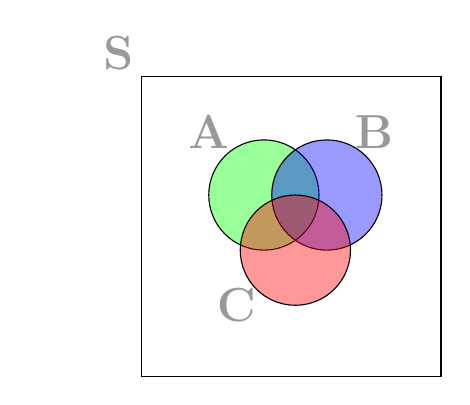
\begin{tikzpicture}
        %% You can adjust the opacity here. For venn diagrams it is convenient to have a low opacity so that you can see intersections
        \begin{scope} [fill opacity = .4]
        %% The draw command knows a lot of shapes. To make a rectangle you just need to specify two diagonal corners. Make sure you always have a semicolon at the end of your draw commands, otherwise latex flips out.
        \draw (0.6,2.5) rectangle (4.4,-1.3);
        %% Similarly, you can make a circle by specifying the center and then the radius. You can also add a fill color, but if you're printing in black and white you'll probably want to remove that line.
        \draw[fill=green, draw = black] (2.15,1) circle (0.7);
        \draw[fill=blue, draw = black] (2.95,1) circle (0.7);
        \draw[fill=red, draw = black] (2.55,0.3) circle (0.7);
        %% We can use the node command to label points. If you put your cursor on "LARGE" or "textbf" a box will drop down with size and text style options.
        \node at (-0.3,2.8) {\LARGE\textbf{\phantom{SB}}};
        \node at (0.3,2.8) {\LARGE\textbf{S}};
        \node at (1.45,1.8) {\LARGE\textbf{A}};
        \node at (3.55,1.8) {\LARGE\textbf{B}};
        \node at (1.8,-0.4) {\LARGE\textbf{C}};
        \end{scope}
        %% And now you have a venn diagram. Yay!
        %\draw[help lines](-5,5) grid (5,-6);    This line can draw the grid lines to help guide you. I use these when I'm writing the code and then delete this line when I publish the pdf.
    \end{tikzpicture}
    \captionof{figure}{$A \cup B \cup C$.}
\end{minipage}%
    \hfill
\begin{minipage}{0.45\textwidth}
    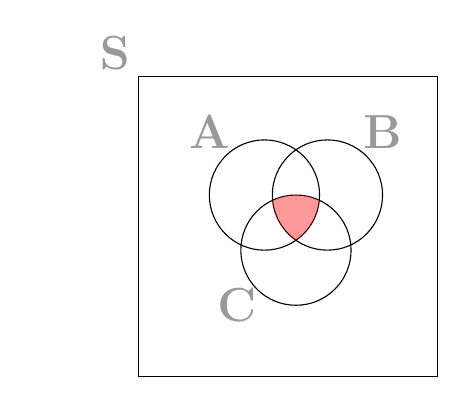
\begin{tikzpicture}
        \begin{scope} [fill opacity = .4]
        \draw (9.4,2.5) rectangle (13.2,-1.3); % add 1.3 to x values
        \draw[fill=none, draw = black] (11,1) circle (0.7);
        \draw[fill=none, draw = black] (11.8,1) circle (0.7);
        \draw[fill=none, draw = black] (11.4,0.3) circle (0.7);

        \begin{scope}
            \clip (11,1) circle (0.7);
            \clip (11.8,1) circle (0.7);
            \fill[red] (11.4,0.3) circle (0.7);
        \end{scope}
        
        \node at (8.3,2.8) {\LARGE\textbf{\phantom{S}}};
        \node at (9.1,2.8) {\LARGE\textbf{S}};
        \node at (10.3,1.8) {\LARGE\textbf{A}};
        \node at (12.5,1.8) {\LARGE\textbf{B}};
        \node at (10.65,-0.4) {\LARGE\textbf{C}};
        \end{scope}
    \end{tikzpicture}
    \captionof{figure}{$A \cap B \cap C$.}
\end{minipage}

\begin{theorem}[\textbf{De Morgan's Laws}]
    \phantom{}
    \begin{enumerate}[label={(\alph*)}]
        \item $\overline{A \cup B} = \overline{A} \cap \overline{B}$
        \item $\overline{A \cap B} = \overline{A} \cup \overline{B}$
    \end{enumerate}
\end{theorem}

\begin{proof}
    \phantom{}  \\
    Use venn diagrams to prove it as an exercise.
\end{proof}




\subsection{Rules for Unions of Events}

\begin{theorem}[\textbf{Rule 4a: Addition Law of Probability or the Sum Rule}]
    \phantom{}  \\
    Let $A$ and $B$ be events (not necessarily mutually exclusive). Then
    \[P(A \cup B) = P(A) +P(B) - P(A \cap B).\]
\end{theorem}

\begin{proof}
    \begin{align*}
        P(A) + P(B) &= \sum_{a \in A} P(a) + \sum_{a \in B} P(a)    \\
                    &= \left(\sum_{a \in A \cap \overline{B} } P(a) + \sum_{a \in A \cap B} P(a)\right)
                       + \left(\sum_{a \in \overline{A} \cap B} P(a) + \sum_{a \in A \cap B} P(a)\right)  \\
                    &= \left(\sum_{a \in A \cap \overline{B}} P(a) + \sum_{a \in A \cap B} P(a)
                             + \sum_{a \in \overline{A} \cap B} P(a)\right) + \sum_{a \in A \cap B} P(a)  \\
                    &= \sum_{a \in A \cup B} P(a) + \sum_{a \in A \cap B} P(a)  \\
                    &= P(A \cup B) + P(A \cap B)
    \end{align*}
    Rearranging the equation, we obtain:
    \[P(A \cup B) = P(A) +P(B) - P(A \cap B),\]
    as desired. This can also be justified by using a Venn diagram. In the expression $P(A) + P(B),$
    the points in $A \cap B$ have their probability counted twice, so they need to be subtracted once.
\end{proof}

\begin{theorem}[\textbf{Rule 4b: Probability of the Union of Three Events}]
    \phantom{}  \\
    Let $A$, $B$ and $C$ be events. then
    \[P(A \cup B \cup C) = P(A) + P(B) + P(C) - P(A \cap B) - P(A \cap C) - P(B \cap C) + P(A \cap B \cap C).\]
\end{theorem}

\begin{proof}
    Use venn diagrams to prove it as an exercise.
\end{proof}

\begin{theorem}[\textbf{Rule 4c: Probability of the Union of $n$ Events}]
    \phantom{}  \\
    A generalization of the above rules to $n$ events $A_1, A_2, \ldots, A_n$. This is often referred to
    as the \textit{inclusion-exclusion principle}.
    \begin{align*}
        P(A_1 \cup A_2 \cup \cdots \cup A_n) = &\sum_{i} P(A_i) - \sum_{i<j} P(A_i \cap A_j)
                                                + \sum_{i<j<k} P(A_i \cap A_j \cap A_k)   \\
                                               &- \sum_{i<j<k<l} P(A_i \cap A_j \cap A_k \cap A_l) + \cdots
    \end{align*}
    (where the subscripts are all distinct).
\end{theorem}

\begin{proof}
    This can be proved using Rule 4a and induction.
\end{proof}

\begin{definition}[\textbf{Mutually Exclusive}]
    Events $A$ and $B$ are \textbf{mutually exclusive} if \[A \cap B = \emptyset.\]
\end{definition}

\begin{remark}
    We can extend this definition to events $A_1, A_2, \ldots, A_n$.
\end{remark}

\begin{example}
    If a die is rolled twice, the events $A = \text{ "2 occurs on the 1st roll"}$ and
    $B = \text{ "total is 10"}$ are mutually exclusive events.
\end{example}

\begin{theorem}[\textbf{Rule 5a: Probability of the Union of Two Mutually Exclusive Events}]
    \phantom{}  \\
    Let $A$ and $B$ be mutually exclusive events. then
    \[P(A \cup B) = P(A) + P(B).\]
\end{theorem}

\begin{theorem}[\textbf{Rule 5b: Probability of the Union of $n$ Mutually Exclusive Events}]
    \phantom{}  \\
    In general, let $A_1, A_2, \ldots, A_n$ be mutually exclusive events. then
    \[P(A_1 \cup A_2 \cup \cdots \cup A_n) = \sum_{i=1}^{n}P(A_i).\]
\end{theorem}

\begin{proof}
    This can be proved from Rule 5a using induction or as an immediate consequence of Rule 4c.
\end{proof}

\begin{theorem}[\textbf{Probability of the Complement of an Event}]
    \phantom{}  \\
    For any event $A$, we have \[P(A) = 1 - P(\overline{A}).\]
\end{theorem}

\begin{proof}
    $A$ and $\overline{A}$ are mutually exclusive and $A \cup \overline{A} = S$, so by Rule 5a,
    \begin{align*}
        P(A \cup \overline{A}) &= P(A) + P(\overline{A})    \\
                             1 &= P(A) + P(\overline{A})    \qquad \left( \text{since $P(A \cup \overline{A}) = 1$} \right)    \\
                 \implies P(A) &= 1 - P(\overline{A}).
    \end{align*}
\end{proof}

\begin{example}
    Two fair dice are rolled. Find the probability that at least one of them turns up a six. \\
    \textbf{Solution 1: } Defining appropriate events: \\
    $A = \left\{  \text{outcome from first die is a 6} \right\}$ and $B = \left\{  \text{outcome from second die is a 6} \right\}$.
    Therefore, either first is a 6 and second is a six OR both give a 6. \\
    $\implies P(A \cup B) = P(A) + P(B) - P(A \cap B) = \frac{1}{6} + \frac{1}{6} - \frac{1 \times 1}{36} = \frac{11}{36}$.

    \textbf{Solution 2:} Using the complement: \\
    $\implies P(\text{at least one 6}) = 1 - P(\text{zero 6s}) = 1 - \frac{5 \times 5}{36} = \frac{11}{36}$.
\end{example}


\subsection{Intersections of Events and Independence}

\begin{definition}[\textbf{Independent and Dependent Events}]
    Events $A$ and $B$ are \textbf{independent events} $\iff P(A \cap B) = P(A)P(B).$
    Otherwise, we call the events \textbf{dependent}.
\end{definition}

Independence means that knowing information about $A$ will not affect the information about $B$.

\begin{definition}
    The events $A_1, A_2, \ldots A_n$ are mutually independent if and only if
    \[P(A_{i_1} \cap A_{i_2} \cap \cdots \cap A_{i_k}) = P(A_{i_1}) P(A_{i_2}) \cdots P(A_{i_k})\]
    for all sets $(i_1, i_2, \ldots, i_k)$ of distinct subscripts chosen $(1, 2, \ldots, n)$.
\end{definition}



\subsection{Conditional Probability}

\begin{definition}[\textbf{Conditional Probability}]
    \phantom{}\\
    The \textbf{conditional probability} of event $A$, given event $B$, is
    \[P(A | B) = \frac{P(A \cap B)}{P(B)}, \quad \text{provided $P(B) > 0.$}\]
\end{definition}

\begin{note}
    $P(A|B) = 1 - P(\overline{A}|B)$.
\end{note}

\begin{theorem}
    \phantom{}  \\
    Suppose $A$ and $B$ are two events defined on a sample space $S$ \st $P(A) > 0$
    and $P(B) > 0.$ Then $A$ and $B$ are independent events $\iff$ either of the following
    statements is true;
    \[P(A|B) = P(A) \quad \text{OR} \quad P(B|A) = P(B).\]
\end{theorem}

\begin{example}[\textbf{exercise}]
    You ask your roommate to water a sickly plant while you are on vacation. Without water, the plant will die with probability 0.8 and with water
    it will die with probability 0.1. Your roommate will remember to water the plant with probability 0.85. \\
    If the plant is alive when you return, what is the probability that your roommate remembered to water it? \\
    \textbf{Answer: } The probability is 0.9623. \\
\end{example}

\begin{example}[\textbf{exercise}]
    The probability a randomly selected male is colour blind is 0.05, whereas the probability a female is colour blind is 0.0025. If the population is
    50\% male, what fraction of the population is colour blind? \\
    \textbf{Answer: } The probability is 0.02625.
\end{example}

\newpage


\subsection{Product Rules, Law of Total Probability and Bayes' Theorem}

\begin{theorem}[\textbf{Rule 7: Product Rules}]
    \phantom{}  \\
    Let $A, B, C, D, \ldots$ be arbitrary events in a sample space. Assume that $P(A) > 0$,
    $P(A \cap B) > 0$, and $P(A \cap B \cap C) > 0$. Then
    \begin{align*}
        P(A \cap B) &= P(A)P(B|A)     \\
        P(A \cap B \cap C) &= P(A)P(B|A)P(C|A\cap B)     \\
        P(A \cap B \cap C \cap D) &= P(A)P(B|A)P(C|A\cap B)P(D|A\cap B\cap C)    \\
        &\vdots
    \end{align*}
\end{theorem}

\begin{proof}
    Use the definition of the conditional probability $P(B|A)$.
\end{proof}

\begin{note}
    Used when finding intersections given conditional probabilities.
\end{note}

\begin{theorem}[\textbf{Rule 8: Law of Total Probability}]
    \phantom{}  \\
    Let $A_1, A_2, \ldots, A_k$ be a partition of the sample space $S$ into disjoint
    (mutually exclusive) events, that is 
    \[A_1 \cup A_2 \cup \cdots \cup A_k = S \quad \text{and} \quad A_i \cap A_j = \emptyset \quad \text{if $i \neq j$.}\]
    Let $B$ be an arbitrary event in $S$. Then
    \begin{align*}
        P(B) &= P(B\cap A_1) + P(B\cap A_2) + \cdots + P(B\cap A_k)    \\
             &= \sum_{i=1}^{k} P(B|A_i) P(A_i).
    \end{align*}
\end{theorem}

\begin{example}[\textbf{exercise}]
    At a police spot check, 10\% of cars stopped have defective headlights and a faulty muffler. 15\% have defective headlights and a
    muffler which is satisfactory. If a car which is stopped has defective headlights, what is the probability that the muffler is also faulty? \\
    \textbf{Answer: } The probability is 0.4.
\end{example}

\pagebreak


\begin{theorem}[\textbf{Bayes' Theorem}]
    \phantom{}  \\
    Suppose $A$ and $B$ are events defined on a sample space $S$. Suppose also that
    $P(B)  > 0$. then
    \[P(A|B) = \frac{P(B|A) P(A)}{P(B)} = \frac{P(B|A) P(A)}{P(B|\overline{A}) P(\overline{A}) + P(B|A) P(A)}.\]
\end{theorem}

\begin{proof}
    \begin{align*}
        \frac{P(B|A) P(A)}{P(B|\overline{A}) P(\overline{A}) + P(B|A) P(A)} &=
        \frac{P(A \cap B)}{P(B \cap \overline{A}) + P(B \cap A)}  \qquad \text{by the Product Rule}   \\
        &= \frac{P(A \cap B)}{P(B)}   \qquad \text{by the Law of Total Probability}  \\
        &= P(A|B).
    \end{align*}
\end{proof}

\begin{remark}
    Bayes' Theorem applies when given "opposite conditions", i.e. we want to find $A|B$ given $B|A$.
\end{remark}



\newpage

\section{Discrete Random Variables}
\subsection{Random Variables and Probability Functions}

\begin{definition}[\textbf{Random Variable}]
    A \textbf{random variable} is a function that assigns a real number to each point
    in a sample space $S$.
\end{definition}

\begin{example}
    Suppose an experiment consists of tossing a coin 3 times. The sample space
    \[S = \left\{ \text{HHH, THH, HTH, HHT, HTT, THT, TTH, TTT} \right\}.\]
    Then $X = $ number of heads that occur would be a random variable, associated with range $A=\left\{ 0,1,2,3 \right\}$. \vspace{-5mm} \\
    \begin{center}
        \begin{tabular}{l|*{1}{c}}
            Events & Outcomes from $S$ \\
            \hline
            $X=0$ & $\left\{ \text{TTT} \right\}$ \\
            $X=1$ & $\left\{ \text{HTT, THT, TTH} \right\}$ \\
            $X=2$ & $\left\{ \text{HHT, HTH, THH} \right\}$ \\
            $X=3$ & $\left\{ \text{HHH} \right\}$
        \end{tabular}
    \end{center}
    Ex. $P(X=1) = P(\text{HTT $\cup$ THT $\cup$ TTH}) = P(\text{HTT}) + P(\text{THT}) + P(\text{TTH}) = \frac{3}{8}$.
\end{example}

\begin{definition}[\textbf{Discrete Random Variables}]
    \textbf{Discrete random variables} take integer values or, more generally, values
    in a countable set.
\end{definition}

\begin{note}
    A set is countable if its elements can be placed in a one-to-one correspondence
    with a subset of the positive integers.
\end{note}

\begin{definition}[\textbf{Continuous Random Variables}]
    \textbf{Continous random variables} take values in some interval of real numbers like
    $(0, 1)$ or $(0, \infty)$ or $(-\infty, \infty)$. 
\end{definition}

\begin{note}
    Cardinality of the real numbers in an interval is NOT countable.
\end{note}

\begin{definition}[\textbf{Probability Function \& Probability Distribution}]
    \phantom{}  \\
    Let $X$ be a discrete random variable with
    $\operatorname{range}{(X)} = A$. The \textbf{probability function} of $X$ is the function
    \[f(x) = P(X = x), \quad \text{defined $\forall \, x \in A$.}\]

    The set of pairs $\{(x, f(x)) : x \in A\}$ is called the \textbf{probability distribution} of $X$.  \\
    All probability functions must have two properties:
    \begin{enumerate}
        \item $f(x) \geq 0 \; \forall x \in A$.
        \item $\dis \sum_{\text{all } x \in A} f(x) =1$.
    \end{enumerate}
\end{definition}

\begin{remark}
    It follows that $0 \leq f(x) \leq 1 \; \forall x \in A$.
\end{remark}

\begin{example}
    The random variable $X$ has probability function given by \vspace{-5mm} \\
    \begin{center}
        \begin{tabular}{l|*{5}{c}}
            $x$ & 0 & 1 & 2 & 3 & 4 \\
            \hline
            $f(x)$ & $0.1c$ & $0.2c$ & $0.5c$ & $c$ & $0.2c$ \\
        \end{tabular}
    \end{center}
    
    \begin{enumerate}[label=(\alph*)]
        \item Find $c$. \\
        \textbf{Solution:} Since $\dis \sum_{\text{all } x \in A} f(x) =1$. Then $0.1c + 0.2c + 0.5c + c + 0.2c = 1$.
        This gives $c = 0.5$.
        \item Find $P(X > 2)$. \\
        \textbf{Solution:} $P(X > 2) = P(X \geq 3) = P(X = 3) + P(X = 4) = c + 0.2c = 1.2c = 0.6$.
    \end{enumerate}
\end{example}

\begin{definition}[\textbf{Cumulative Distribution Function}]
    The \textbf{cumulative distribution function} of the discrete random variable $X$
    is the function usually denoted by $F(X)$.
    \[F(x) = P(X \leq x) \quad \text{defined $\forall \, x \in \R$}\]
\end{definition}

In general, $F(x)$ can be obtained from $f(x)$ using:
\[F(x) = P(X \leq x) = \displaystyle \sum_{u\leq x} f(u).\]

\vspace{-5mm}

\begin{theorem}[\textbf{Properties of a CDF $F(x)$}]
    \phantom{}
    \begin{enumerate}
        \item $F(x)$ is a non-decreasing function of $x \; \forall x \in \R$. For example, $P(X \leq 8)$ cannot be less than $P(X \leq 7)$.
        \item $0 \leq F(x) \leq 1 \; \forall x \in \R$.
        \item $\dis \lim_{x \to -\infty} F(x) = 0$ and $\dis \lim_{x \to \infty} F(x) = 1$.
    \end{enumerate}
\end{theorem}

We can also obtain $f(x)$ from $F(x)$. If $X$ takes on integer values then for values $x$ \st $x \in A$ and $x-1 \in A$, 
\[f(x) = F(x) - F(x-1).\]
In other words:
\[P(X = x) = P(X \leq x) - P(X \leq x-1).\]
We notice that $f(x)$ represents the size of the jump in $F(x)$ at the point $x$.


\textbf{Plots of $f(x)$ and $F(x)$} \\
For discrete random variables, the cdf $F(x)$ is represented as a step function, whereas the pf $f(x)$ is represented by a histogram.


\subsection{Discrete Uniform Distribution}

\textbf{Physical Setup:}  Suppose the range of $X$ is $\{a, a + 1, \ldots, b\}$ where $a$ and $b$ are integers and suppose all values are equally probable.
Then $X$ has a Discrete Uniform distribution on the set $\{a, a + 1, \ldots, b\}$. The variables $a$ and $b$ are called the parameters of the distribution.

\textbf{Probability Function:} There are \(b - a + 1\) values in the set \(\{a, a + 1, \ldots, b\}\) so the probability of each value must be \(\frac{1}{b - a + 1}\) in order that \(\dis \sum_{x=a}^{b} f(x) = 1\). Therefore

\[
    f(x) = P(X = x) = 
    \begin{cases} 
        \frac{1}{b - a + 1} & \text{for } x = a, a + 1, \ldots, b \\
        0 & \text{otherwise}
    \end{cases}
\]

\begin{example}
    Suppose a fair die is thrown once and let $X$ be the number on the face. Find the cumulative distribution function of $X$. \\
    \textbf{Solution:} $x = 1,2,3,4,5,6$ and $X \sim \text{Unif}[1,6]$.
    \[
        f(x) = P(X = x) = 
        \begin{cases} 
            \frac{1}{6} & \text{for } x = 1,2,\ldots,6 \\
            0 & \text{otherwise}
        \end{cases}
    \]
    $F(1) = P(X \leq 1) = P(X = 1) = \frac{1}{6}$ and $F(2) = P(X \leq 2) = P(X = 1) + P(X = 2) = \frac{2}{6}$. So
    \[
        F(x) = P(X \leq x) = 
        \begin{cases} 
            0 & \text{for } x < 1 \\
            \frac{[x]}{6} & \text{for } 1 \leq x < 6 \\
            1 & \text{for } x \geq 6 
        \end{cases}.
    \]
\end{example}


\subsection{Hypergeometric Distribution}

\textbf{Physical Setup:}
We have \textbf{\textit{N objects}} that can be classified into exactly \textbf{\textit{two}} distinct types, “success” (S) vs. “failure” (F).

$r =$ \# of successes \quad and \quad $N-r=$ \# of failures.

We pick \underline{$n$} objects at random \textbf{without} replacement. If X represents the number of successes, then X has a hypergeometric distribution.

\begin{example}
    Of the 120 applicants for a job, only 80 are qualified. In total, 5 applicants are picked at random for an interview. If X represents the number of qualified
    applicants that are interviewed, then X has a hypergeometric distribution, where:
    \begin{itemize}
        \item $N = 120$
        \item $r = 80$ since $N - r = 40$
        \item $n = 5$
        \item Possible values of $x$ are 0, 1, 2, 3, 4, 5.
    \end{itemize}
\end{example}

\textbf{Probability Function:} Using counting techniques we note there are \(\binom{N}{n}\) points in the sample space
\(S\) if we don't consider order of selection. There are \(\binom{r}{x}\) ways to choose the \(x\) success objects from the
\(r\) available and \(\binom{N-r}{n-x}\) ways to choose the remaining \((n - x)\) objects from the \((N - r)\) failures. Hence

\[
    f(x) = P(X = x) = \frac{\binom{r}{x} \binom{N-r}{n-x}}{\binom{N}{n}}
\]
where $x \geq \operatorname{max}(0,n-(N-r))$ and $x \leq \operatorname{min}(r,n)$.

\begin{note}
    Do not need to memorize this formula because it will be easy to realize based on the given context.
\end{note}

\begin{example}[\textbf{Above Continued}]
    \phantom{}\\
    Find the probability that only two of the five selected will be qualified for the job. \vspace{2mm} \\ 
    \textbf{Solution:} $P(X = 2) = \dis \frac{\binom{80}{2} \binom{40}{3}}{\binom{120}{5}} = 0.164$.
\end{example}

\begin{example}
    In the game of Texas Hold'em, players are each dealt two private cards, and five community cards are dealt face-up on the table.
    Each player makes the best 5-card hand they can with their two private cards and the five community cards.
    What is the probability that a particular player can make a flush of spades (i.e. 5 spades or more)?

    \textbf{Solution:} $X = \#$ of spades among 7 cards. $N = 52$, $r = 13$, $N-r = 39$, $n = 7$, and $x = 0,1,2,\ldots ,7$. \vspace{-4mm}
    \begin{align*}
        P(X \geq 5) &= P(X=5)+ P(X=6) + P(X=7) \\
        &= \dis \frac{\binom{13}{5}\binom{39}{2} + \binom{13}{6}\binom{39}{1} + \binom{13}{7}\binom{39}{0}}{\binom{52}{7}} \\
        &= 0.0076.
    \end{align*}
\end{example}

\begin{example}
    A manufacturer of auto parts just shipped 25 auto parts to a dealer. Later, it found out that 5 of those parts were defective. By the time the company
    manager contacted the dealer, 4 auto parts from that shipment had been sold. What is the probability that 3 of those 4 parts were good parts and one was defective?

    \textbf{Solution:} $X = \#$ of defectives selected, $N = 25$, $r = 5$, and $n = 4$. \vspace{-3mm}
    \[
        P(X = 1) = \dis \frac{\binom{5}{1}\binom{25-5}{4-1}}{\binom{25}{4}} = 0.45.
    \]
\end{example}


\subsection{Binomial Distribution}

\textbf{Physical Setup:} Suppose an experiment has \textbf{\textit{two}} possible outcomes, ``success'' and ``failure''.
Let $P(\text{Success}) = p$ and hence $P(\text{Failure}) = 1-p$. Repeat the experiment \textbf{\textit{$n$ independent}} times.
Let $X$ be the number of successes obtained, we say $X$ has a \textbf{\textit{Binomial distribution}}.


We write \( X \sim Bin(n, p) \) with $n$ total trials and $p$ probability to success.

\begin{note}
    The \textbf{\textit{n individual}} experiments are called “trials” or “Bernoulli trials” and the process is
    called a Bernoulli process or Binomial process. \\
\end{note}


Underlying assumptions for the Binomial Distribution: (Tims)
\begin{itemize}
    \item T: Two outcomes
    \item I: Independent trials
    \item M: Multiple trials
    \item S: Same probability of success in each trial.
\end{itemize}

\begin{example}
    A fair coin is tossed 12 times. Let X be the number of heads obtained. Then:
    \begin{itemize}
        \item Two outcomes: Head (success) vs. Tail (failure)
        \item Independent trials: flips are independent of each other
        \item Multiple trials: $n = 12$
        \item Same $P(\text{Success})$ in each trial = $p$ = 0.5.
    \end{itemize}
    Thus, $X \sim Bin(12, 0.5)$ and $x = 0,1,2, \ldots ,12$. \\
\end{example}

\textbf{Probability Function:} There are $\binom{n}{x}$ arrangements of $x$ successes and $(n-x)$ failures over the $n$ trials.
Each arrangement has probability $p^x(1-p)^{n-x}$. Therefore,
\[f(x) = P(X=x) = \binom{n}{x}p^x(1-p)^{n-x} \quad \text{for $x = 0,1,\ldots ,n$ and $0 < p < 1$}.\]

\begin{remark}
    Check the above function by using the property that $\displaystyle \sum_{\text{all $x$}} f(x) = 1$ for $0 < p < 1$.
\end{remark}

\begin{example}
    Seventy-five percent of students at a college with a large student population use Instagram.
    A sample of five students from this college is selected. What is the probability that at least 3 use Instagram?

    \textbf{Solution:} $X = \#$ of students that use Instagram among 5 selected. Then $X \sim Bin(5,0.75)$ for $x=0,1,\ldots ,5$.
    \[P(X \geq 3) = P(X=3) + P(X=4) + P(X=5) = 1- P(X \leq 2).\]
\end{example}

\begin{remark}
    \phantom{}\\
    The probability of at least `x': $P(X \geq x) = 1 - P(X \leq (x-1))$. \\
    The probability of more than `x': $P(X > x) = 1 - P(X \leq x)$.
\end{remark}

\textbf{Binomial vs. Hypergeometric}

Similarities
\begin{itemize}
    \item Both have two types of outcomes, success and failure.
    \item The experiment is repeated $n$ times.
    \item $X$ records the number of successes.
\end{itemize}

Differences
\begin{itemize}
    \item Binomial reqires \textbf{independent} trials, where the probability of success is the same in each trial.
    \item In Hypergeometric, the draws are made from a fixed number of objects $N$ \textbf{without} replacement. Hence, the trials are \textbf{not independent}. \\
\end{itemize}

\begin{example}
    Suppose we have 20 cans of drinks placed in a big ice container such that the labels are not visible. It is known that 12
    are coke and 8 are juice. We randomly pick 10 cans. Find the probability that 3 are coke.

    \textbf{Solution:} Assume the draws are down without replacement (correct approach here). We have $N=20$, $r=12$, $N-r=8$, and $n=10$. So $X \sim \text{Hypergeo}(20, 12, 10)$.
    
    Thus, $P(X=3) = \frac{\binom{12}{3}\binom{8}{7}}{\binom{20}{10}} = 0.00953.$
\end{example}

\begin{remark}
    If $N$ is large and $n$ (number of objects being drawn) is relatively small, then binomial can be used as an approximation for the hypergeometric. \\

    \textbf{Rule of thumb:} If the sample size (number of trials) $n$ is at most $5\%$ of the population size, the experiment can be analyzed as though it were exactly a Binomial experiment.
\end{remark}

\begin{example}
    Megan audits 130 clients during a year and finds irregularities for 26 of them.
    \begin{enumerate}[label=(\alph*)]
        \item Give an expression for the probability that 2 clients will have irregularities when 6 of her
        clients are picked at random. \\
        \textbf{Solution:} Let $X = \#$ of clients with irregularities among 6 selected, $N=130$, $r=26$, $n=6$.
        \[P(X=2) = \frac{\binom{26}{2}\binom{130-26}{6-2}}{\binom{130}{6}} = 0.251.\]
        \item Evaluate your answer to (a) using a suitable approximation. \\
        \textbf{Solution:} $X \sim \text{Bin}(6,\frac{26}{130})$. Then we have
        \[P(X=2)=\binom{6}{2}\left(\frac{26}{130}\right)^2 \left(1-\frac{26}{130}\right)^{6-2} = 0.246 \approx 0.25.\]
        Notice that $\frac{n}{N} = \frac{6}{130} = 0.046 < 5\%$.
    \end{enumerate}
\end{example}


\subsection{Negative Binomial Distribution}

\textbf{Physical Setup:} similar to the Binomial Distribution. Do experiment until we obtain $k$ successes. However now, $X$ records the number of
failures obtained before the $k$th success, $X \sim \text{NB}(k,p)$.

\begin{example}
    Draw cards with replacement until you get 3 Aces. Let $X = \#$ of Non-Aces that we obtain before the third Ace. Then the distribution of $X$ is
    $X \sim \text{NB}(k=3, p=P(\text{Success})=\frac{4}{52})$ with $x =  0,1, \ldots$.
\end{example}


\textbf{Probability Function:} In total, we have $x$ failures and $k$ successes, so there are $x+k$ trials, the last trial \textbf{MUST} be a success.
Hence in the first $x+k-1$ trials, we observe $x$ failures and $(k-1)$ successes. Therefore, there are $\binom{x+k-1}{x} = \binom{x+k-1}{k-1}$ arrangements, each arrangement has probability $p^k(1-p)^x$.
Hence \[f(x) = P(X=x) = \binom{x+k-1}{x}p^k(1-p)^x \quad \text{for $x = 0,1,\ldots$ and $0 < p < 1$}.\]

\begin{note}
    An alternate version of Negative Binomial Distribution defined $X$ to be the total number of trials needed to get the $k$th success. We'll have something like: $X-4 \sim \text{NB}(k,p)$, 
    where 4 is just an example here, representing the number of successes before the 5th success.
\end{note}

\textbf{Binomial vs. Negative Binomial}
\begin{itemize}
    \item \textbf{Binomial:} We know that we have $n$ trials in advance but do not
    know the \# of successes we will obtain until after the experiment.
    \item \textbf{Negative Binomial:} We know the number $k$ of successes in advance but do
    not know the \# of trials that will be needed to obtain this \# of success until after the experiment.
\end{itemize}


\pagebreak

\begin{example}
    Two athletic teams, $A$ and $B$, play a best-of-three series of games (i.e the first team to win two games is the overall winner). Suppose team $A$ is the
    stronger team and will win any game with probability 0.6, independently from other games. Let $X$ be the number of games lost before Team $A$ wins twice.
    Find the probability that Team $A$ is the overall winner.

    \textbf{Solution:} $X \sim \text{NB}(2, 0.6)$. \vspace{-5mm}
    \begin{align*}
        \text{Probability} &= P(X = 0) + P(X = 1) \\
        &= \binom{0+2-1}{0}(0.6)^2(0.4)^0 + \binom{1+2-1}{1}(0.6)^2(0.4)^1
    \end{align*}
\end{example}

\begin{example}
    A startup is looking for 5 investors. Each investor will independently agree with probability 20\%.
    A founder asks investors one at a time until they get 5 ``yes''.
    Let $X$ be the total $\#$ of investors asked. Find $f(x)$ and $f(6)$.

    \textbf{Solution:} Let $Y = \#$ of ``No''s until the 5th yes is obtained. Then $Y \sim \text{NB}(5,0.2)$, $y = 0,1,2,\ldots$.
    And $X = Y + 5$. \vspace{-5mm}
    \begin{align*}
        f_X(x) &= P(X=x) \\
        &= P(X = x = Y + 5) \\
        &= P(Y = x - 5) \\
        &= f_Y(x-5) \\
        &= \binom{x-5+5-1}{x-5}p^5(1-p)^{x-5} \\
        &= \binom{x-1}{x-5}p^5(1-p)^{x-5} \text{, $x = 5,6,7,\ldots$}
    \end{align*}

    $\dis f_x(6) = P(X = 6) = \binom{6-1}{6-5}0.2^5(1-0.2)^{6-5} = 0.00128$.
    
\end{example}



\subsection{Geometric Distribution}

\textbf{Physical Setup:} Independent Bernoulli trials, each having two possible outcomes (Success vs. Failure). 
The probability, $p$, of success is the same each time. However, $X = \#$ of failures before the \textbf{FIRST} success
(i.e. a Negative Binomial distribution with $k=1$). 

We write $X \sim \text{Geo}(p)$.


\textbf{Probability Function:} There is only the one way with $x$ failures followed by 1 success.
\[f(x) = P(X=x) = (1-p)^x p \quad \text{for $x = 0,1,\ldots$ and $0<p<1$}.\]

\begin{remark}
    Alternatively, substitute $k=1$ in $f(x)$ for the Negative Binomial. \\
\end{remark}


In summary, we notice that Binomial, Negative Binomial and Geometric all assume:
\begin{enumerate}
    \item Two outcomes in each trial.
    \item Independent Trails.
    \item Each trial has the same probability of success. \\
\end{enumerate}



\begin{example}
    A company receives $60\%$ of its orders over the internet.
    \begin{enumerate}[label=(\alph*)]
        \item What is the probability that the fifth order received is the first internet order? \\
        \textbf{Solution:} Let $X = \#$ of orders not over the internet untill the first internet order. Then $X \sim \text{Geo}(0.6)$, $x=0,1,2,\ldots$.
        We have $P(X = 4) = (0.6)^1 (1-0.6)^4$.
        \item What is the probability that the eighth order received is the fourth internet order? \\
        \textbf{Solution:} Let $Y =$ total number of orders before the 4th internet order. $Y \sim \text{NB}(4, 0.6)$. Then $\dis f_y(4) = P(Y = 4) = \binom{4+4-1}{4}(0.6)^4(1-0.6)^4$. Since we have 4 successes and 4 failures.
        
        Alternatively, $Y =$ number of non-internet orders before 4th internet. Then $Y-3 \sim \text{NB}(4,0.6)$.
    \end{enumerate}
\end{example}


\subsection{Poisson Distribution from Binomial}

\textbf{Physical Setup:} $X = \#$ of events of some type. The events occur according to some rate $\mu$, where $\mu > 0$.
We write $X \sim \text{Poisson}(\mu)$.

\textbf{Probability Function:} 
\[
    f(x) = P(X = x) = \dis \frac{e^{-\mu} \mu^x}{x!} \quad \text{for } x = 0, 1, \ldots
\]
where $\mu > 0$.

\begin{remark}
    Poisson arises from Binomial when $n \to \infty$ and $p \to 0$, $X \sim \text{Bin}(n, \frac{\mu}{n})$. $(\mu = np)$
\end{remark}


\begin{example}
    Consider the Tim Hortons event ``Roll up the Rim''. We are told that 1 in 9 cups are winners.
    Say you buy 100 cups, assuming they are independent, and use the Poisson approximation to solve for the probability that you get no more than 10 winning cups.

    \textbf{Solution:} Find the exact probability using Binomial.

    Let $X = \#$ of winning cups among 100. Then $X \sim \text{Bin}(100, \frac{1}{9})$. We have $P(X \leq 10) = 0.439$.

    Now, use Poisson approximation. We have $\mu = np = 100 \times \frac{1}{9} = \frac{100}{9}$. Then

    $P(X \leq 10) = P(X = 0) + P(X = 1) + \cdots + P(X = 10) = e^{-\frac{100}{9}}\left[ \frac{\mu^0}{0!} + \frac{\mu^1}{1!} + \cdots + \frac{\mu^{10}}{10!}\right] = 0.447$. \\
\end{example}

\begin{example}
    If you buy a lottery ticket in 50 lotteries, in each of which your chance of winning a prize is
    1/100, what is the (approximate) probability that you will win a prize
    \begin{enumerate}[label=(\alph*)]
        \item At least once,
        \item Exactly once,
        \item At least twice?
    \end{enumerate}

    \textbf{Solution:} We have $\mu = np = 50 \times \frac{1}{100} = 0.5$.
    \begin{enumerate}[label=(\alph*)]
        \item $P(X \geq 1) = 1 - P(X = 0) = 1 - \frac{e^{-0.5}(0.5)^0}{0!} = 0.3935$.
        \item $P(X = 1) = \frac{e^{-0.5}(0.5)^1}{1!} = 0.3023$.
        \item $P(X \geq 2) = 1 - P(X \leq 1) = 1 - P(X = 0) - P(X = 1) = 0.09017$. \\
    \end{enumerate}
\end{example}


\begin{note}
    \phantom{}\
    \begin{enumerate}
        \item If $p$ is close to 1, we can still use Poisson to approximate Binomial, simply by interchanging the labels ``success'' and ``failure''. Now, we can get $P(\text{success})$ is close to 0.
    \end{enumerate}
\end{note}

\pagebreak

\subsection{Poisson Distribution from Poisson Process}

\begin{definition}[\textbf{Poisson Process}]
    \phantom{}  \\
    The following three conditions together define a \textbf{Poisson Process}:
    \begin{enumerate}
        \item \textbf{Independence:} the number of occurrences in non-overlapping intervals are independent.
        \item \textbf{Individuality:} $P(\text{2 or more events in $(t, t+\Delta t)$}) = o(\Delta t)$ (close to 0) as $\Delta t \to 0$.
        \item \textbf{Homogeneity or Uniformity:} Events occur at a homogeneous (uniform) rate $\lambda$ over time so that
        $P(\text{one event in $(t, t+\Delta t)$}) = \lambda \Delta t + o(\Delta t)$.
    \end{enumerate}
\end{definition}

In a Poisson process with rate of occurrence $\lambda$, the number of event occurrences $X$ in a time interval of length $t$
has a Poisson distribution with $\mu = \lambda t$.

\[f(x) = P(X=x) = \dis \frac{e^{-\lambda t} (\lambda t)^x}{x!} \text{, $x=0,1,2,\ldots$}\]


\textbf{Interpreting $\mu$ and $\lambda$.}
\begin{enumerate}
    \item $\lambda$ refers to the intensity or rate of occurrence. It represents the average rate of occurrence of events per unit of time.
    \item $\mu = \lambda t$ represents the average number of occurrences in $t$ units of time. \\
\end{enumerate}


\begin{example}
    Suppose earthquakes recorded in Ontario each year follow a Poisson process with an average of 6 per year.
    What is the probability that 7 will be recorded in a two year period?

    \textbf{Solution:} Let $X = \#$ of earthquakes in the two year period ($t = 2$). And the intensity of earthquakes is $\lambda = 6$ per year.
    So $\mu = \lambda t = 6 \times 2 = 12$ in two years. Then, $f(7) = \frac{e^{-12} 12^7}{7!} = 0.0437$. \\
\end{example}


The Poisson process also applies when ``events'' occur randomly in space. If $X$ represents the number of events in a volume or area in space of size $v$,
and if $\lambda$ is the average number of events per unit voilume (or area), then $X$ has a Poisson distribution with $\mu = \lambda v$.

The model is valid when we replace ``time'' by ``volume'' or ``area''.

\pagebreak

\begin{example}
    Coliform bacteria occur in a river water with an average intensity of 1 bacteria per 10 cubic centimeters (cc) of water. Find:
    \begin{enumerate}[label=(\alph*)]
        \item The probability there are no bacteria in a 20cc sample of water which is tested.
        
        \textbf{Solution:} Let $X = \#$ of Coliform bacteria observed in a specified volume. Then $X \sim \text{Poi}(\lambda = 1 \text{ per 10cc})$.
        We have $\mu = \lambda t = \frac{1}{10} \times 20 = 2$ per 20cc. So $P(X = 0) = \frac{e^{-2} 2^0}{0!} = e^{-2}$.
        \item The probability there are 5 or more bacteria in a 50cc sample.
        
        \textbf{Solution:} $\mu = \lambda t = \frac{1}{10} \times 50 = 5$ per 50cc. Then \vspace{-5mm}
        \begin{align*}
            P(X \geq 5) &= 1 - P(X \leq 4) \\
            &= 1 - \left[ P(X=0) + \cdots + P(X=4) \right] \\
            &= 1 - e^{-5} \left[ \frac{5^0}{0!} + \frac{5^1}{1!} + \cdots + \frac{5^4}{4!} \right].
        \end{align*}
    \end{enumerate}
\end{example}


\textbf{Distinguishing Poisson from Binomial and Other Distributions}

\begin{enumerate}
    \item Can we specify in advance the maximum value which $X$ can take? \\
    If we can, then the distribution is NOT Poisson. If there is no fixed upper limit, then might be Poisson.
    \item Does it make sense to ask how often the event did not occur? \\
    If it does make sense, the distribution is NOT Poisson. If it does not make sence, then might be Poisson.
\end{enumerate}


\subsection{Combining Other Models with the Poisson Process}

\begin{example}
    A very large (essentially infinite) number of ladybugs is released in a large orchard.
    They scatter randomly so that on average a tree has 6 ladybugs on it. Trees are all the same size.
    \begin{enumerate}[label=(\alph*)]
        \item Find the probability a tree has > 3 ladybugs on it. \\
        \textbf{Solution:} Poisson distribution with $\lambda = 6$ and $v = 1$ (that is, any tree has a ``volume'' of one unit). So $\mu = \lambda v = 6$.
        Then $P(X > 3) = 1 - P(X \leq 3) = 1 - e^{-6}\left[ \frac{6^0}{0!} + \frac{6^1}{1!} + \frac{6^2}{2!} + \frac{6^3}{3!} \right] = 0.8488$.
        \item When 10 trees are picked at random, what is the probability that 8 of these trees have > 3 ladybugs on them? \\
        \textbf{Solution:} Binomial distribution where success means >3 ladybugs on a tree. We have $X \sim \text{Bin}(10, 0.8488)$.
        Then $P(X = 8) = \binom{10}{8}(0.8488)^8 (1-0.8488)^2 = 0.2772$.
        \item Trees are checked until 5 with > 3 ladybugs are found. Let $X$ be the total number of trees checked. Find the probability function, $f(x)$. \\
        \textbf{Solution:} $X-5 \sim \text{NB}(5, 0.8488)$ with $(x-5)$ failures. Then
        \begin{align*}
            f(x) &= \binom{x-5+5-1}{x-5}(0.8488)^5 (1-0.8488)^{x-5} \\
            &= \binom{x-1}{x-5}(0.8488)^5 (0.1512)^{x-5} \\
            &= \binom{x-1}{4}(0.8488)^5 (0.1512)^{x-5} \text{, $x = 5,6,7,\ldots$}
        \end{align*}
        \item Find the probability a tree with > 3 ladybugs on it has exactly 6. \\
        \textbf{Solution:} Let $A = {\text{6 ladybugs}}$ and $B = {\text{more than 3 ladybugs}}$. \\
        Then, $P(A|B) = \frac{P(A \cap B)}{P(B)} = \frac{P(A)}{P(B)} = \frac{\frac{e^{-6} 6^6}{6!}}{0.8488} = 0.1892$.
        \item On 2 trees there are a total of $t$ ladybugs. Find the probability that $x$ of these are on the first tree. \\
        \textbf{Solution:}
        \begin{align*}
            P(\text{$x$ on first tree} | \text{total of $t$}) &= \frac{P(\text{$x$ on first tree} \cap \text{total of $t$})}{P(\text{total of $t$})} \\
            &= \frac{P(\text{$x$ on first tree} \cap \text{$t-x$ on second tree})}{P(\text{total of $t$})} \\
            &= \frac{P(\text{$x$ on first tree}) \cdot P(\text{$t-x$ on second tree})}{P(\text{total of $t$})}
        \end{align*}
        Use Poisson distribution with $\mu = 6 \times 2 = 12$ in the denominator since there are two trees.
        \begin{align*}
            &= \frac{ \left( \frac{e^{-6} 6^x}{x!} \right) \left( \frac{e^{-6} 6^{t-x}}{(t-x)!} \right) }{\frac{e^{-12} 12^t}{t!}} \\
            &= \frac{t!}{x!(t-x)!} \left( \frac{6}{12} \right)^x \left( \frac{6}{12} \right)^{t-x} \\
            &= \binom{t}{x} \left( \frac{1}{2} \right)^x \left( 1 - \frac{1}{2} \right)^{t-x} \text{ for $x = 0,1,\ldots, t$}. 
        \end{align*}
        \begin{remark}
            We can also let $X = \#$ of ladybugs on the first tree, then $X \sim \text{Bin}(t, 0.5)$. Since the probability of a ladybug on the first tree is just 0.5 as there are two trees.
        \end{remark}
    \end{enumerate}
\end{example}


\subsection{Summary of Probability Functions for Discrete Random Variables}

\begin{center}
    \begin{tabular}{l l}
        \textbf{Name} & \textbf{Probability Function} \\ \hline \addlinespace \addlinespace
        Discrete Uniform & $\dis f(x) = \frac{1}{b - a + 1} \quad \text{for } x = a, a + 1, a + 2, \ldots, b \quad (b > a)$ \vspace{10pt}    \\
        Hypergeometric & $\dis f(x) = \frac{\binom{r}{x} \binom{N-r}{n-x}}{\binom{N}{n}} \quad \text{for } x = \max(0, n - (N - r)), \ldots, \min(n, r)$ \vspace{10pt} \\
        Binomial & $\dis f(x) = \binom{n}{x} p^x(1 - p)^{n-x} \quad \text{for } x = 0, 1, 2, \ldots, n \quad (0 < p < 1)$ \vspace{10pt}  \\
        Negative Binomial & $\dis f(x) = \binom{x+k-1}{x} p^k(1 - p)^x \quad \text{for } x = 0, 1, 2, \ldots \quad (0 < p < 1)$ \vspace{10pt}    \\
        Geometric & $\dis f(x) = p(1 - p)^x \quad \text{for } x = 0, 1, 2, \ldots \quad (0 < p < 1)$ \vspace{10pt}   \\
        Poisson & $\dis f(x) = \frac{e^{-\mu}\mu^x}{x!} \quad \text{for } x = 0, 1, 2, \ldots \quad (\mu > 0)$ \vspace{30pt}  \\
    \end{tabular}
\end{center}

% An example of drawing probability function table:   \\
% \begin{tabular}{l|*{5}{c}}
%     $x$ & 1 & 2 & 3 & 4 & 5 \\
%     \hline
%     $F(x)$ & $0.1k$ & $0.2$ & $0.5k$ & $k$ & $4k^2$ \\
% \end{tabular}



\newpage

\section{Computational Methods and the Statistical Software R}
Not covered material.

\section{Expected Value and Variance}
\subsection{Summarizing Data on Random Variables}

\textbf{Frequency Histogram}
\begin{itemize}
    \item Symmetric: mean = median
    \item Right-skewed: mean > median
    \item Left-skewed: mean < median
\end{itemize}
\begin{definition}[\textbf{Sample}]
    A set of observed outcomes $x_1, \ldots, x_n$ for a random variable $X$
    is a \textbf{sample}.
\end{definition}

\begin{definition}[\textbf{Arithmetic Mean or Sample Mean}]
    The \textbf{mean} of $n$ outcomes $x_1, \ldots, x_n$ for a randome variable
    $X$ is \[\bar{x} = \dis \sum_{i=1}^n \frac{x_i}{n}.\]
\end{definition}

\begin{definition}[\textbf{Median}]
    The \textbf{median} of a sample is a value \st half the results are below it and
    half above it, when the results are arranged in numerical order.
\end{definition}

\begin{note}
    If there are even number of values. The median is the mean of the two middle values.
\end{note}

\begin{definition}[\textbf{Mode}]
    The \textbf{mode} of the sample is the value which occurs most often. 
\end{definition}

\begin{note}
    There can be multiple modes.
\end{note}


\subsection{Expectation of a Random Variable}

\begin{definition}[\textbf{Expected Value (Expectation)}]
    Let $X$ be a discrete random variable with $\operatorname{range}{(X)} = A$ and
    probability function $f(x)$. The \textbf{expected value} of $X$ is given by
    \[\mu = \expect{X} = \sum_{x \in A} xf(x).\]   
\end{definition}

\begin{theorem}[\textbf{Expected Value of $g(X)$}]
    \phantom{}  \\
    Let $X$ be a discrete random variable with $\operatorname{range}{(X)} = A$ and
    probability function $f(x)$. The \textbf{expected value} of some function $g(X)$
    of $X$ is given by
    \[\expect{g(X)} = \sum_{x \in A} g(x)f(x).\]    
\end{theorem}


\begin{note}
    \phantom{}\
    \begin{enumerate}
        \item Interpret $\expect{g(X)}$ as the average value of $g(X)$ in an infinite series of repetitions of the process where $X$ is defined.
        \item $\expect{g(X)}$ may be a value that $g(X)$ never takes.
        \item $\expect{X}$ is NOT a random variable like $X$ but a non-random constant.
        \item Suppose $X$ takes values from 1 to 10. Then $\expect{X}$ cannot exceed 10 or smaller than 1.
    \end{enumerate}
\end{note}

\begin{theorem}[\textbf{Linearity Properties of Expectation}]
    \phantom{}  \
    \begin{enumerate}
        \item For constants $a$ and $b$, \[\dis \expect{ag(X) + b} = a\expect{g(X)} + b.\]
        \item For constants $a$, $b$ and two functions $g_1$, $g_2$, 
        \[\expect{ag_1(X) + bg_2(X)} = a\expect{g_1(X)} + b\expect{g_2(X)}.\]
    \end{enumerate}
\end{theorem}

\begin{note}
    For constant $a$, we have $\expect{a} = a$.
\end{note}

\pagebreak 

\begin{example}
    Suppose we have the random variable $X$ \st $f_X(x) = \frac{x}{10}$, $x = 1,2,3,4$. Find $\expect{X(5-X)}$.

    \textbf{Solution:} \\
    $\expect{X(5-X)} = \expect{5X - X^2} = 5\expect{X} - \expect{X^2} = 5 \left[ (1 \times \frac{1}{10}) + \cdots + (4 \times \frac{4}{10}) \right] - \left[ (1^2 \times \frac{1}{10}) + \cdots + (4^2 \times \frac{4}{10}) \right] \\ = 5 \times 3 - 10 = 5$.
\end{example}


\subsection{Some Applications of Expectation}

\begin{example}
    A local television station sells 15sec, 30sec, and 60sec advertising spots. Let $X$ denote the length of a randomly selected commercial appearing on this
    station, and suppose that the probability distribution of $X$ is given by
    \begin{center}
        \begin{tabular}{l|*{3}{c}}
            $x$ & 15 & 30 & 60 \\
            \hline
            $f(x)$ & $0.1$ & $0.3$ & $0.6$ \\
        \end{tabular}
    \end{center}

    \begin{enumerate}[label=(\alph*)]
        \item Find $\expect{X}$. \\
        \textbf{Solution:} $\expect{X} = \displaystyle \sum_{\text{all $x$}} xf(x) = (15 \times 0.1) + (30 \times 0.3) + (60 \times 0.6) = 46.5$ seconds.
        \item If a 15s spot sells for \$500, a 30s spot for \$800, and a 60s spot for \$1000, find the average amount paid for commercials appearing on this station. \\
        \textbf{Solution:} $\expect{Y} = (500 \times 0.1) + (800 \times 0.3) + (1000 \times 0.6) = \$890$. \\
    \end{enumerate}
    
\end{example}

\subsection{Means and Variances of Distributions}

\begin{definition}[\textbf{Expectation for Probability Models}]
    \phantom{}\
    \begin{enumerate}
        \item Binomial: $\expect{X} = np$.
        \item Poisson: $\expect{X} = \lambda t = \mu$.
        \item Discrete Uniform: $\expect{X} = \dis \frac{a+b}{2}$.
        \item Hypergeometric: $\expect{X} = \dis \frac{nr}{N}$.
        \item Negative Binomial: $\expect{X} = \dis \frac{k(1-p)}{p}$.
        \item Geometric: $\expect{X} = \dis \frac{1-p}{p}$.
    \end{enumerate}
\end{definition}

\begin{definition}[\textbf{Variance}]
    The \textbf{variance} of a random variable $X$, denoted by $\Var{X}$ or $\sigma^2$, is
    \[\sigma^2 = \Var{X} = \expect{(X - \mu)^2}.\]
\end{definition}

\begin{note}
    Variance is the average square of the distance from the mean ($\text{units}^2$).
\end{note}

The definition of variance is not efficient to use for calculation of $\Var{X}$, whereas
the following two results are often useful:
\begin{theorem}
    \phantom{}\
    \begin{enumerate}
        \item $\dis \Var{X} = \expect{X^2} - \left[\expect{X}\right]^2 = \expect{X^2} - \mu^2$
        \item $\dis \Var{X} = \expect{X(X - 1)} + \expect{X} - \left[\expect{X}\right]^2 = \expect{X(X - 1)} + \mu - \mu^2$
    \end{enumerate}
\end{theorem}

\begin{definition}[\textbf{Standard Deviation}]
    The \textbf{standard deviation} of a random variable $X$ is
    \[\sigma = \operatorname{sd}{(X)} = \sqrt{\Var{X}} = \sqrt{\expect{(X - \mu)^2}}\]
\end{definition}

\begin{figure}[htbp]
    \center
    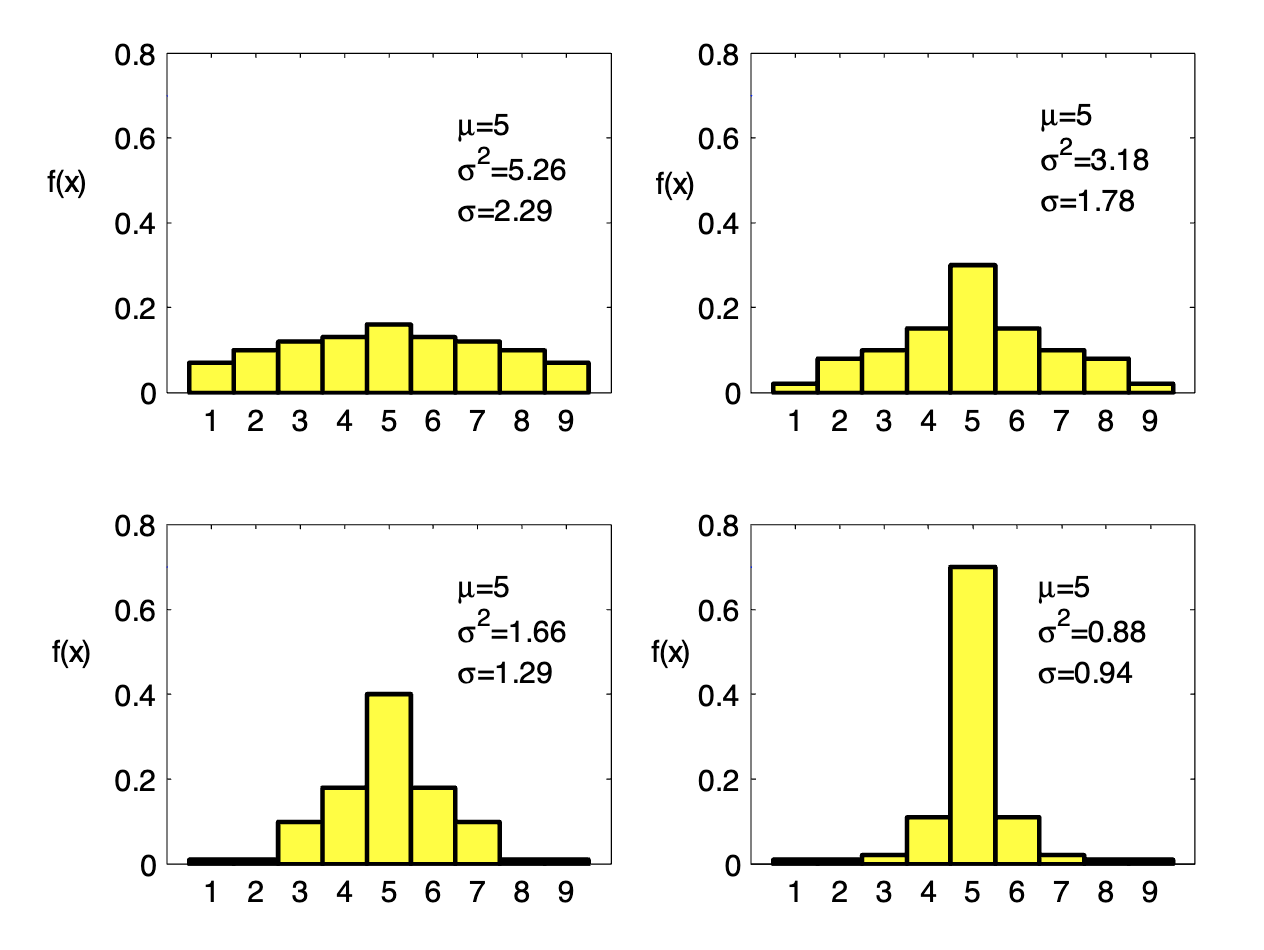
\includegraphics[scale=0.55]{img/var-and-sd.png}
    \caption{How $\Var{X}$ or $\operatorname{sd}(X)$ reflects the spread of a probability histogram.}
\end{figure}

\begin{definition}[\textbf{Variance for Probability Models}]
    \phantom{}\
    \begin{enumerate}
        \item Binomial: $\Var{X} = np(1-p)$.
        \item Poisson: $\Var{X} = \mu$.
        \item Discrete Uniform: $\Var{X} = \dis \frac{(b-a+1)^2 - 1}{12}$.
        \item Hypergeometric: $\Var{X} = \dis \frac{nr}{N} \left( 1 - \frac{r}{N} \right) \frac{N-n}{N-1}$.
        \item Negative Binomial: $\Var{X} = \dis \frac{k(1-p)}{p^2}$.
        \item Geometric: $\Var{X} = \dis \frac{1-p}{p^2}$.
    \end{enumerate}
\end{definition}

\begin{theorem}[\textbf{Properties of Mean and Variance}]
    \phantom{}  \\
    If $a$ and $b$ are constants and $Y = aX + b$, then
    \[\mu_Y = \expect{Y} = a\expect{X} + b = a\mu_X + b\] and
    \[\sigma_Y^2 = \Var{Y} = a^2\Var{X} = a^2\sigma_X^2,\]
    where $\mu_X = \expect{X}$, $\sigma_X^2 = \Var{X}$, $\expect{Y} = \mu_Y$, and $\Var{Y} = \sigma_Y^2.$
\end{theorem}

\begin{note}
    For constant $a$, we have $\Var{a} = 0$.
\end{note}




\newpage

\section{Continous Random Variables}
\subsection{General Terminology and Notation}

Continuous random variables take values on some interval of real numbers. We have $P(X = x) = 0$ for each $x$, because $P(X = a) = \displaystyle \int_{a}^{a} f(x) \, dx = 0$. 

We use the cumulative distribution function $F(x)$ and the probability density function $f(x)$ to describe a continuous random variable.

\begin{definition}[\textbf{Cumulative Distribution Function (c.d.f.)}]
    \phantom{}
    \[F(x) = P(X \leq x).\]
\end{definition}

\begin{theorem}[\textbf{Properties of a c.d.f.}]
    \phantom{}\
    \begin{enumerate}
        \item $F(x)$ is defined $\forall x \in \R$.
        \item $F(x)$ is a non-decreasing function of $x$.
        \item $\dis \lim_{x \to -\infty} F(x) = 0$ and $\dis \lim_{x \to \infty} F(x) = 1$.
        \item  $P(a \leq X \leq b) = F(b) - F(a)$.
    \end{enumerate}
\end{theorem}

\begin{note}
    Since $P(X = x) = 0$ for each $x$, we have \vspace{-3mm}
    \[P(a < X < b) = P(a \leq X \leq b) = P(a \leq X < b) = P(a < X \leq b) = F(b) - F(a).\]
\end{note}

\begin{definition}[\textbf{Probability Density Function (p.d.f.)}]
    \phantom{}\\
    The \textbf{probability density function} $f(x)$ for a continous random variable $X$
    is the derivative \[f(x) = \frac{\dd{F(x)}}{\dd{x}},\]
    where $F(x)$ is the cumulative distribution function for $X$.
\end{definition}

\begin{note}
    From the way in which $X$ was generated that $f(x)$ represents the \textbf{relative likelihood} of (small intervals around) different $x$-values (outcomes).
\end{note}

\pagebreak


\begin{theorem}[\textbf{Properties of a p.d.f.}]
    \phantom{}\\
    Assume that $f(x)$ is a continuous function of $x$ at  all points for which $0 < F(x) < 1$.
\begin{enumerate}
    \item $\dis P(a \leq X \leq b) = F(b) - F(a) = \int_{a}^{b} f(x) \, dx$. \vspace{1mm}
    \item $f(x) \geq 0$ (since $F(x)$ is non-decreasing, so its derivative should be non-negative). \vspace{1mm}
    \item $\displaystyle \int_{-\infty}^{\infty} f(x) \, dx = \displaystyle \int_{\text{all $x$}} f(x) \, dx = 1$.
    \item $F(x) = \displaystyle \int_{-\infty}^{x} f(u) \, du$ (this is property 1 with $a = -\infty$). \\
\end{enumerate}
\end{theorem}

\begin{definition}[\textbf{Quantiles and Percentiles}]
    \phantom{}\\
    Suppose $X$ is a continuous random variable with cumulative distribution function $F(x).$
    The $p$th quantile of $X$ (or of the distribution) is the value $q(p)$, \st $P\left[X \leq q(p)\right] = p.$    \\
    The value $q(p)$ is also called the $100$th percentile of the distribution. If $p = 0.5$, then
    $m = q(0.5)$ is called the median of $X$ or the median of the distribution.
\end{definition}

\begin{remark}
    The \textbf{Median} is the value $m$ such that
    \[
        F(m) = \displaystyle \int_{-\infty}^{m} f(x) \, dx = 0.5 = \displaystyle \int_{m}^{\infty} f(x) \, dx, \text{ which is the 50th percentile.}
    \]
\end{remark}

\begin{example}
    Let
    \[
        F(x) = 
        \begin{cases} 
        0 & \text{for } x \leq 0 \\
        \frac{x}{4} & \text{for } 0 < x \leq 4 \\
        1 & \text{for } x > 4 
        \end{cases}
    \]
    \begin{enumerate}[label=(\alph*)]
        \item Solve for $f(x)$. \\
        \textbf{Solution:} $f(x) = \frac{\dd}{\dd{x}} \left( F(x) \right) = \frac{\dd}{\dd{x}} \left( \frac{x}{4} \right) = \frac{1}{4}$ for $0 < x \leq 4$. Note that outside this interval $f(x)$ is defined to be 0.
        \item Solve for the 90th percentile, i.e. solve for the value of $x$ \st the area under the curve to its left is 0.9. \\
        \textbf{Solution:} Note that the $f(x) = \frac{1}{4}$ is a constant function. \\
        We need to solve for $x$: $F(x) = P(X \leq x) = 0.9$. So, $\frac{1}{4} x = 0.9 \implies x = 3.6$.
    \end{enumerate}
\end{example}

\pagebreak

\begin{example}
    Let $X$ be a continuous random variable with p.d.f.
    \[
        f(x) = 
        \begin{cases} 
        c(4x - 2x^2) & \text{for } 0 < x < 2 \\
        0 & \text{otherwise}
        \end{cases}
    \]
    Find
    \begin{enumerate}[label=(\alph*)]
        \item the constant $c$.
        \item $F(x)$.
        \item $P(X > 1)$.
    \end{enumerate}

    \textbf{Solution:} 
    \begin{enumerate}[label=(\alph*)]
        \item 
        \begin{align*}
            \displaystyle \int_{-\infty}^{\infty} f(x) \, dx &= 1 \\
            \displaystyle \int_{0}^{2} c(4x - 2x^2) \, dx &= 1 \\
            c \left[ 2x^2 - \frac{2x^3}{3} \right]_0^2 &= 1 \\
            &\vdots \\
            c &= \frac{3}{8}
        \end{align*}
        \item $F(X) = P(X \leq x) = \displaystyle \int_{-\infty}^{x} f(u) \, du = \displaystyle \int_{0}^{x} \frac{3}{8} (4u - 2u^2) \, du = \frac{3}{8} \left[ 2u^2 - \frac{2u^3}{3} \right]_0^2 = \frac{3}{8} \left( 2x^2 - \frac{2x^3}{3} \right)$.
        
        Therefore, we have 
        \[
            F(x) = 
            \begin{cases} 
            0 & x \leq 0 \\
            \frac{3}{8} \left( 2x^2 - \frac{2x^3}{3} \right) & 0 < x < 2 \\
            1 & x \geq 2
            \end{cases}.
        \]
        \item $P(X > 1) = \displaystyle \int_{1}^{\infty} f(x) \, dx = \displaystyle \int_{1}^{2} f(x) \, dx = \cdots = 0.5$.
        
        OR \\
        $P(X > 1) = 1 - P(X \leq 1) = 1 - F(1) = \cdots = 0.5$.
    \end{enumerate}
\end{example}

\pagebreak

\textbf{Defined Variables or Change of Variables:}  \\
Suppose we know the p.d.f. or c.d.f. for a continous random variable $X$, we sometimes want to find
the p.d.f. or c.d.f. for some other random variable $Y$, a function of $X$. The procedure is summarized below.
\begin{enumerate}
    \item Write the c.d.f. of $Y$ as a function of $X$.
    \item Use $F_X(x)$ to find $F_Y(x)$. Then if you want the p.d.f. $f_Y(y)$, you can differentiate $F_Y(x)$.
    \item Find the range of values of $y$.
\end{enumerate}

\begin{example}
    $X$ is a continuous random variable having
    \[
        f(x) = \frac{1}{4} \text{ for $0 < x \leq 4$} \quad \text{and} \quad F(x) = \frac{x}{4} \text{ for $0 < x \leq 4$}.
    \]
    Let $Y = \frac{1}{X}$. Find the p.d.f. of $Y$.


    \textbf{Solution:} \\
    Step 1: \vspace{-3mm}
    \begin{align*}
        F_Y(y) = P(Y\leq y) &= P(\frac{1}{X} \leq y) \\
        &= P(X \geq \frac{1}{y}) \\
        &= 1 - P(X \leq \frac{1}{y}) \\
        &= 1 - F_X(\frac{1}{y})
    \end{align*}

    Step 2: 
    \[
        F_Y(y) = 1 - F_X(\frac{1}{y}) = 1 - \frac{\frac{1}{y}}{4} = 1 - \frac{1}{4y}.
    \]
    We can differentiate $F_Y(y)$ to obtain $f_Y(y)$. 
    \[
        f_Y(y) = \frac{\dd}{\dd{y}} \left( 1 - \frac{1}{4y} \right) = \frac{1}{4y^2} \text{ for $y \geq \frac{1}{4}$}.
    \]
    Step 3: note that $x \in (0,4]$, so $y = \frac{1}{x} \in [\frac{1}{4},\infty)$.
\end{example}

\pagebreak

\begin{definition}[\textbf{Mean, and Variance for Continous Random Variables}]
    \phantom{}  \\
    If $X$ is a continous random variable, then we define
    \[
        \expect{g(X)} = \displaystyle \int_{-\infty}^{\infty} g(x)f(x) \, dx.
    \]
\end{definition}

\begin{remark}[\textbf{Mean and Variance}]
    \phantom{}\
    \begin{itemize}
        \item $\expect{X} = \displaystyle \int_{-\infty}^{\infty} xf(x) \, dx$, which is the average of the distribution.
        \item $\sigma^2 = \Var{X} = \expect{(X - \mu)^2} = \expect{X^2} - \left( \expect{X} \right)^2$.
    \end{itemize}
\end{remark}

\begin{example}
    If $X$ is a continuous random variable having p.d.f 
    \[f(x) = \frac{1}{4} \quad \text{for $0 < x \leq 4$}.\]
    Find $\expect{X}$ and $\Var{X}$.

    \textbf{Solution:} $\expect{X} = 0 + \displaystyle \int_{0}^{4} x \left( \frac{1}{4} \right) \, dx + 0= 2$,
    and $\expect{X^2} = 0 + \displaystyle \int_{0}^{4} x^2 \left( \frac{1}{4} \right) \, dx + 0 = \frac{16}{3}$.

    Finally, we have $\dis \Var{X} = \frac{16}{3} - 2^2 = \frac{4}{3}$. \\
\end{example}

\begin{example}[\textbf{Exercise!}]
    Let $X$ be a random variable with p.d.f. given by
    \[
        f(x) = 
        \begin{cases} 
        k \sqrt{x} & \text{for } 0 \leq x \leq 1 \\
        \frac{k}{x^4} & \text{for } x > 1 \\
        0 & \text{otherwise}
        \end{cases}
    \]
    \begin{enumerate}[label=(\alph*)]
        \item Find the constant k. \quad \textbf{Ans:} $k = 1$
        \item Find the c.d.f. $F(x)$ for all values of $x$. \quad
        \textbf{Ans:} 
        $F(x) = 
        \begin{cases} 
            0 & x \leq 0 \\
            \frac{2}{3} x^{3/2} & 0 \leq x \leq 1 \\
            1 - \frac{1}{3x^3} & x > 1
        \end{cases}$
        \item Find $P(\frac{1}{3} < X < 3)$. \quad \textbf{Ans:} 0.8594
        \item Calculate $\expect{X}$ and $\Var{X}$. \quad \textbf{Ans:} $\expect{X} = 0.9$ and $\Var{X} = 0.48$
    \end{enumerate}
\end{example}


\subsection{Continous Uniform Distribution}

\textbf{Physical setup:} $X$ is a continuous random variable takes values in $[a,b]$ (it doesn't matter whether the interval is open or closed) with all subintervals of a fixed length being equally likely.

Then $X$ has a continuous uniform distribution. We write $X \sim \text{U}(a,b)$, for $b > a$ and $a,b \in \R$.


\textbf{P.D.F. and C.D.F}:
Since all points are equally likely (intervals contained in $[a,b]$ of a given length all have the same probability), it must be a constant function $f(x) = k$ for $a \leq x \leq b$ and for some constant $k$.
Next, we need $\displaystyle \int_{a}^{b} f(x) \, dx = 1 \implies k(b-a) = 1$.

\[
    f(x) = 
    \begin{cases} 
    \frac{1}{b-a} & \text{for } a \leq x \leq b \\
    0 & \text{otherwise}
    \end{cases}.
\]

It follows that the c.d.f. is
\[
    F(x) = 
    \begin{cases} 
    0 & x < a \\
    \frac{x - a}{b - a} & a \leq x \leq b \\
    1 & x > b
    \end{cases}
\]

\begin{itemize}
    \item $\expect{X} = \displaystyle \int_{a}^{b} x \left( \frac{1}{b-a} \right) \, dx = \frac{a+b}{2}$.
    \item $\Var{X} = \dis \frac{(b-a)^2}{12}$. \\
\end{itemize}

\begin{example}
    Tansforming a random variable with a different continuous distribution to obtain a uniform distribution.

    Suppose $X$ has the continuous p.d.f. $f(x) = 0.1 e^{-0.1x}$ for $x > 0$. We will show that the new random variable $Y = e^{-0.1X}$ has a uniform distribution, $\text{U}(0,1)$.

    \textbf{Solution:} \\
    $F_Y(y) = P(Y \leq y) = P(e^{-0.1X} \leq y) = P(X \geq -10\ln{y}) = 1 - P(X < -10 \ln{y}) = 1 - F_X(-10 \ln{y})$.

    Next, since $x > 0$, we have $F_X(x) = \displaystyle \int_{0}^{x} 0.1e^{-0.1u} \, du = 1 - e^{-0.1x}$. 
    
    So $F_Y(y) = 1 - \left[ 1 - e^{-0.1 \left( -10 \ln{y} \right)} \right] = y$ for $0 < y < 1$, since the range of $X$ is $(0,\infty)$.

    Thus, $f_Y(y) = \frac{\dd}{\dd{y}} (F_Y(y)) = 1$ for $0 < y < 1$, which implies $Y \sim \text{U}(0,1)$.
\end{example}


\subsection{Exponential Distribution}

\textbf{Physical sestup:} In a Poisson Process for events in time let $X = $ length of time we wait until the first
occurrence. Then X has an exponential distribution.

\begin{note}
    Recall that the $\#$ of occurrences in a fixed time has a Poisson distribution.
\end{note}

\begin{example}
    If phone calls to a fire station follows a Poisson process, then the length of time between phone calls follows an exponential distribution.
\end{example}


\textbf{P.D.F. and C.D.F}:
\begin{align*}
    F(x) = P(X \leq x) &= P(\text{time to 1st occurrence} \leq x) \\
    &= 1 - P(\text{time to 1st occurrence} > x) \\
    &= 1 - P(\text{0 occurrences in $(0,x)$}) \\
    &= 1 - \frac{e^{-\lambda x}(\lambda x)^0}{0!} \\
    &= 1 - e^{-\lambda x} \quad \text{for $x > 0$}.
\end{align*}
Note that the number of occurrences has a Poisson distribution with $\mu = \lambda x$, where $\lambda$ is the average rate of occurrence.

Then,
\[
    f(x) = \frac{\dd}{\dd{x}} \left( F(X) \right) = \lambda e^{-\lambda x} \quad \text{for $x > 0$}.
\]


\textbf{Alternate Form:} Let $\theta = \frac{1}{\lambda}$, so $\theta = $ average waiting time to an occurrence. 
We have
\[
    F(x) = 
    \begin{cases} 
    1 - e^{\frac{-x}{\theta}} & x > 0 \\
    0 & x \leq 0
    \end{cases}
\]

\[
    f(x) = 
    \begin{cases} 
    \frac{1}{\theta} e^{\frac{-x}{\theta}} & x > 0 \\
    0 & x \leq 0
    \end{cases}.
\]
where $\theta > 0$. We write $X \sim \text{Exp}(\theta)$. 

\begin{example}
    If $\lambda = 5$ occurrences per hour, then $\theta = \frac{1}{5}$ means: have to wait an average of $\frac{1}{5}$th of an hour to see an occurrence. 
\end{example}

\vspace{2mm}

To find the mean and variance, we can use the properties of the Gamma Function. 
\begin{definition}[\textbf{The Gamma Function}]
    \[\Gamma{(\alpha)} = \int_{0}^{\infty} x^{\alpha - 1}e^{-x} \, dx\]
    is called the gamma function of $\alpha$, where $\alpha > 0$.
\end{definition}

\textbf{Properties of the gamma function:}
\begin{enumerate}
    \item $\Gamma{(\alpha)} = (\alpha - 1)\Gamma{(\alpha - 1)}$ for $\alpha > 1$.
    \item $\Gamma{(\alpha)} = (\alpha - 1)!$ if $\alpha$ is a positive integer.
    \item $\Gamma{(\frac{1}{2})} = \sqrt{\pi}$. \\
    (This can be proved using double integration.) \\
\end{enumerate}

Goind back to the exponential distribution, we have
\begin{itemize}
    \item $\expect{X} = \theta = \dis \frac{1}{\lambda}$.
    \item $\Var{X} = \theta^2 = \dis \frac{1}{\lambda^2}$.
\end{itemize}

\begin{remark}
    Leave proofs as exercises, use the Gamma function. \\ \phantom{} \\
\end{remark}

\begin{example}
    The average amount of time in hours that a computer survives before breaking down is 100 hours. What is the probability that
    \begin{enumerate}[label=(\alph*)]
        \item A computer will function between 50 and 150 hours before breaking down?
        \item It will function for fewer than 100 hours?
        \item If a computer survives more than 100 hours, what is the probability it survives an additional 50 hours?
    \end{enumerate}

    \pagebreak

    \textbf{Solution:}
    \begin{enumerate}[label=(\alph*)]
        \item Let $X =$ the length of time waited until 1st breakdown. Then $X \sim \text{Exp}(\theta = 100 \text{ hours})$. \vspace{-2mm}
        \begin{align*}
            P(50 \leq X \leq 150) = P(50 < x < 150) &= P(X \leq 150) - P(X \leq 50) \\
            &= F(150) - F(50) \\
            &= \left( 1 - e^{\frac{-150}{100}} \right) - \left( 1 - e^{\frac{-50}{100}} \right) \\
            &= e^{\frac{-50}{100}} - e^{\frac{-150}{100}}
        \end{align*}
        \item $P(X < 100) = F(100) = 1 - e^{\frac{-100}{100}} = 1 - \frac{1}{e} = 0.6321$. \\
        \item \phantom{A} \vspace{-3mm}
        \begin{align*}
            P(X > 100 + 50 | X > 100) &= \frac{P(X > 150 \cap X > 100)}{P(X > 100)} \\
            &= \frac{P(X > 150)}{P(X > 100)} \\
            &= \frac{1 - P(X \leq 150)}{1 - P(X \leq 100)} \\
            &= \frac{1 - \left( 1 - e^{\frac{-150}{100}} \right)}{1 - \left( 1 - e^{\frac{-100}{100}} \right)} \\
            &= e^{\frac{-50}{100}} \left( = P(X > 50) \right)
        \end{align*}
    \end{enumerate}
\end{example}

\begin{remark}
    Part (c) illustrates the ``\textbf{memoryless property}'' of the Exponential distribution:
    \[
        P(X > c + b | X > b) = P(X > c).
    \]
    Given that you have waited $b$ units of time for the next event, the probability you wait an additional $c$ units of time \textbf{does not} depend on $b$ but only depends on $c$. \\
\end{remark}

\pagebreak

\begin{example}[\textbf{Exercise}]
    Suppose that the length of a phone call in minutes is an exponential random variable with parameter $\lambda = \frac{1}{10}$. If someone arrives immediately ahead of you at a public telephone booth, find the probability that you will have to wait
    \begin{enumerate}[label=(\alph*)]
        \item More than 10 mins. \quad \textbf{Ans: $e^{-1}$}
        \item Between 10 and 20 mins. \quad \textbf{Ans: $e^{-1} - e^{-2} = 0.233$}
        \item If you have been waiting for more than 10 mins, what is the probability you have to wait for more than an additional 5 mins? \quad \textbf{Ans: $e^{-\frac{1}{2}}$} \\
    \end{enumerate}
\end{example}


\subsection{A Method for Computer Generation of Random Variables}

Not covered material.

\pagebreak

\subsection{Normal Distribution}

\textbf{Physical setup:} A random variable $X$ defined on $(-\infty, \infty)$ has a Normal distribution if it has p.d.f. of the form
\[
    f(x) = \frac{1}{\sqrt{2\pi\sigma}} e^{-\frac{1}{2}\left(\frac{x-\mu}{\sigma}\right)^2}, \quad x \in \R.
\]
where $\mu \in \R$ and $\sigma > 0$ are parameters. 

\begin{itemize}
    \item $\expect{X} = \mu$.
    \item $\Var{X} = \sigma^2$.
\end{itemize}


We write $X \sim \text{N}(\mu,\sigma^2)$.

\begin{figure}[!htb]
    \begin{minipage}{0.48\textwidth}
      \centering
      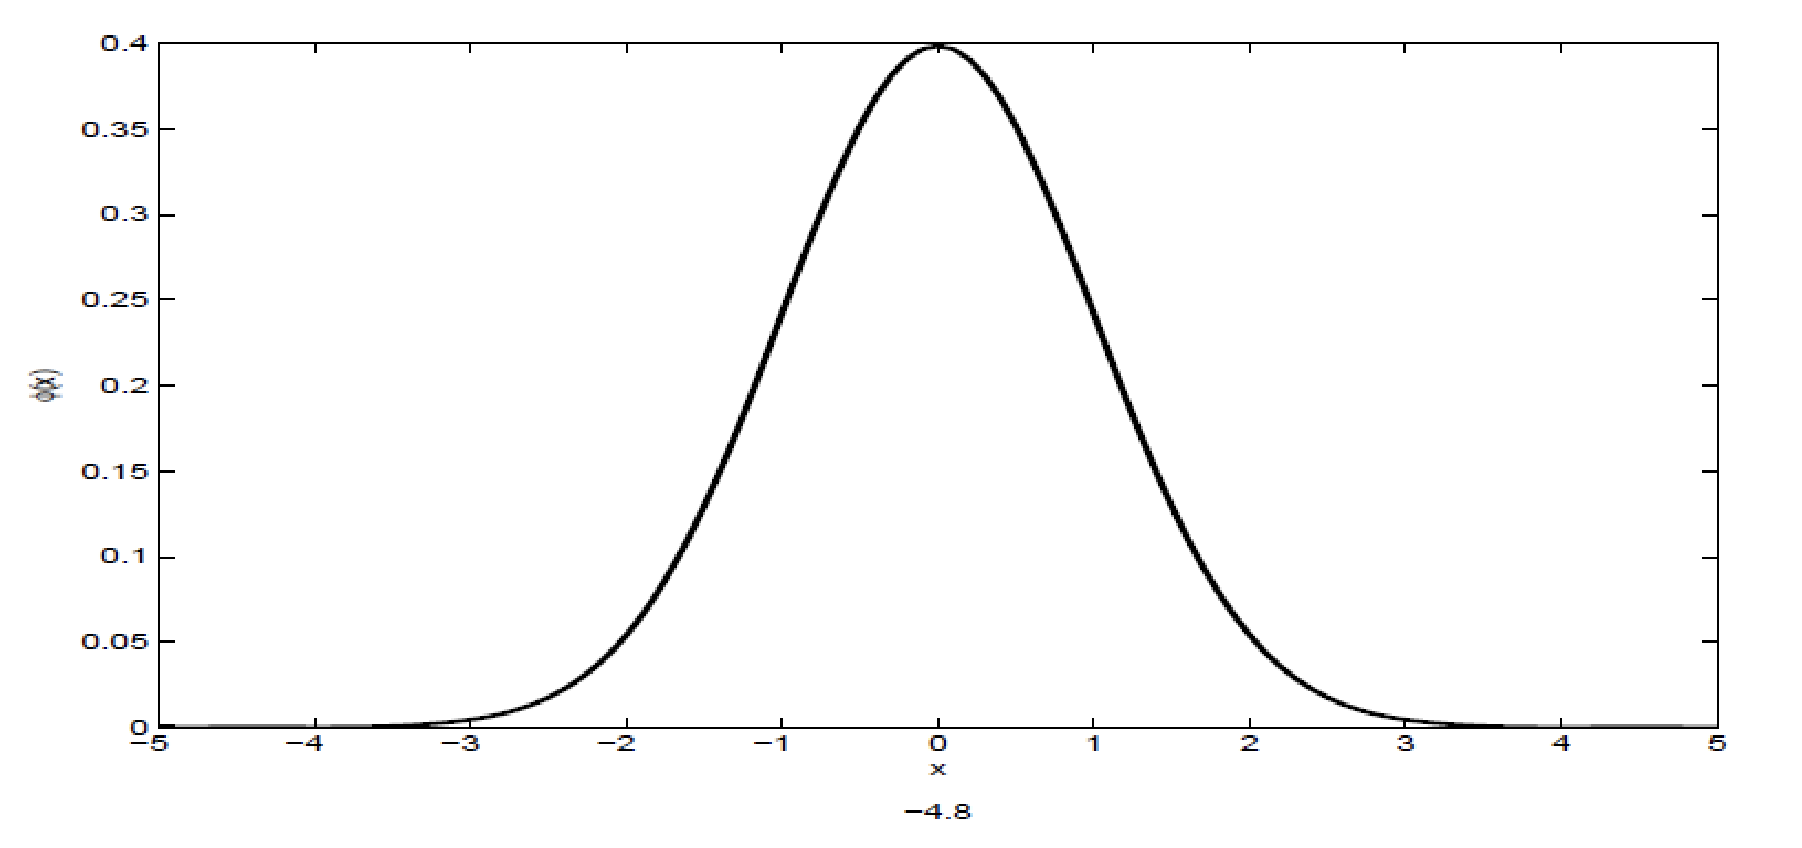
\includegraphics[width=1.05\linewidth]{img/standard-normal.png}
      \caption{The Standard Normal $N(0,1)$ p.d.f.}
    \end{minipage}\hfill
    \begin{minipage}{0.48\textwidth}
      \centering
      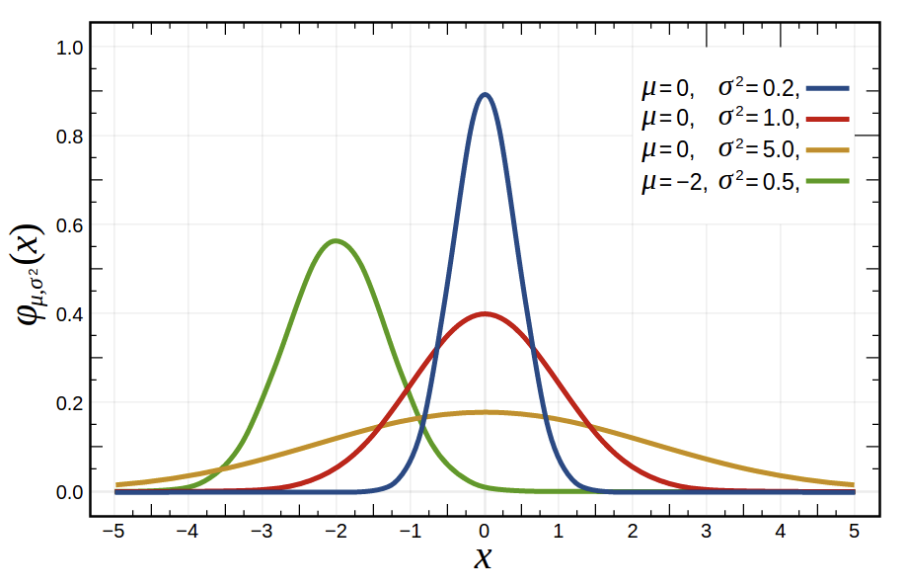
\includegraphics[width=0.9\linewidth]{img/different-normal.png}
      \caption{Some p.d.f.s}
    \end{minipage}
 \end{figure}

 \begin{note}
    For the first figure, we have $\mu = 0$ and $\sigma^2 = 1$. Normal distributions are symmetric about the mean (the line $x = \mu$), so 50\% on each side.
 \end{note}

 \vspace{3mm}

\textbf{Effects of the Mean and the Variance}

\begin{figure}[!htb]
    \begin{minipage}{0.48\textwidth}
      \centering
      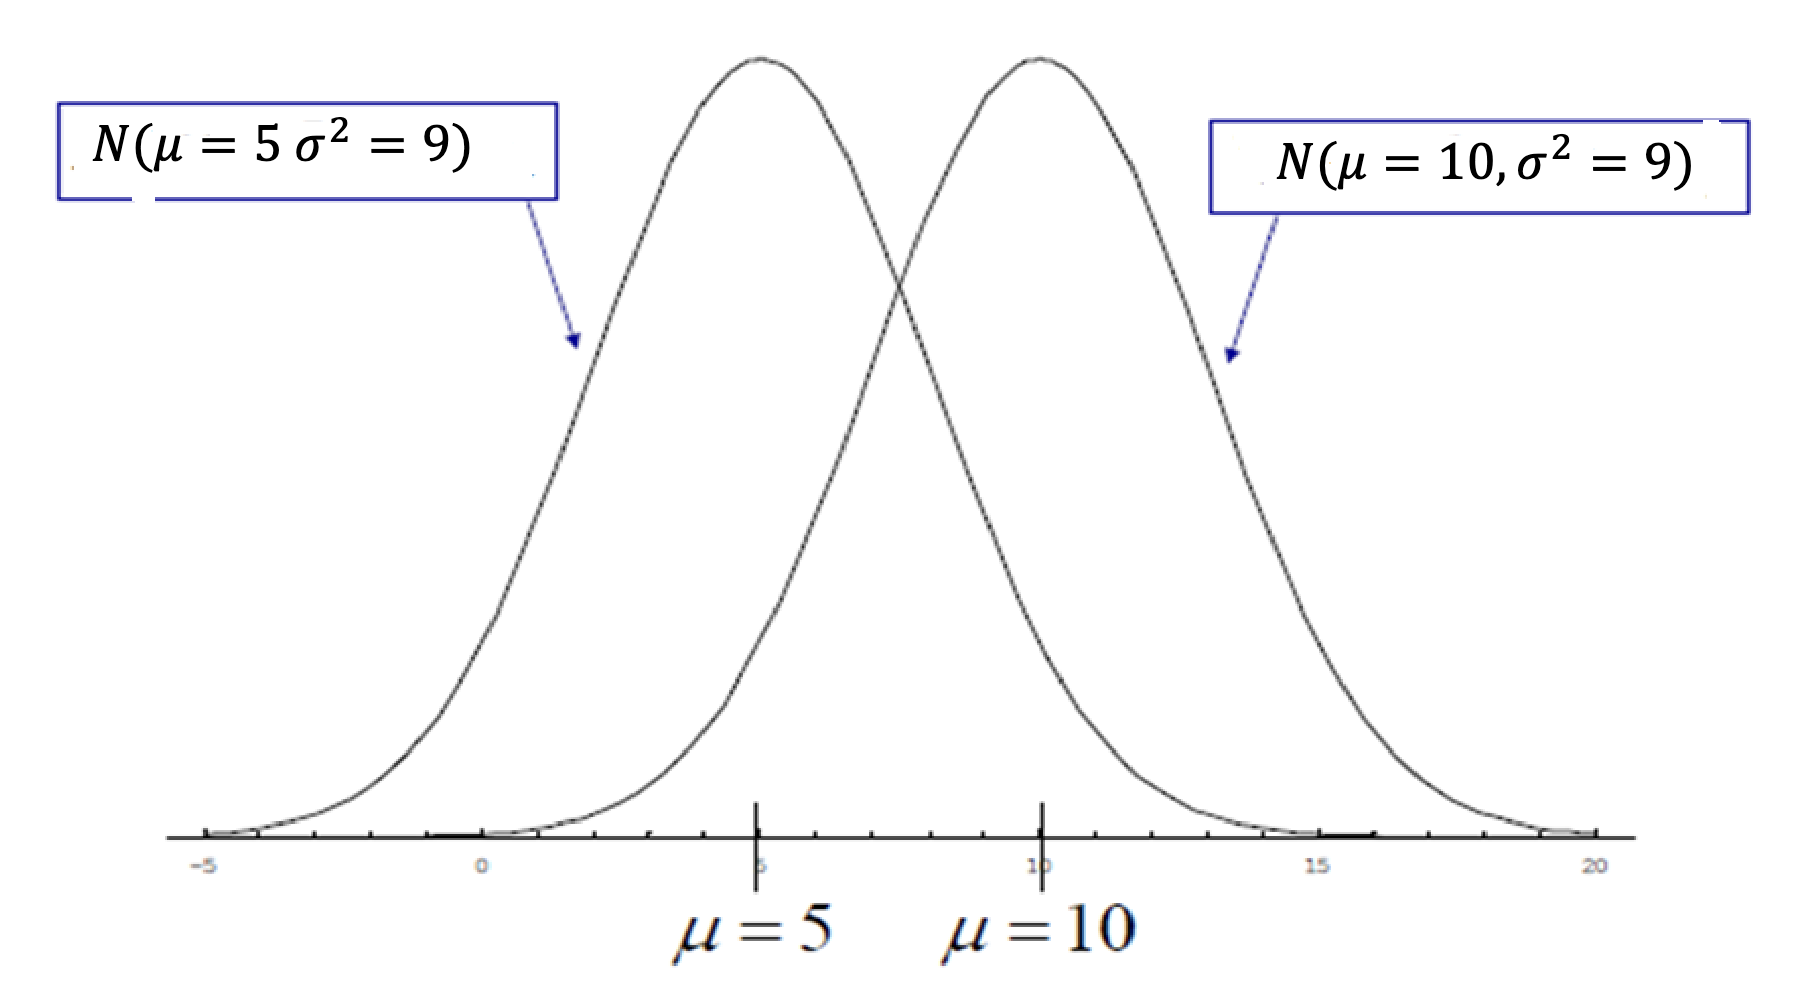
\includegraphics[width=1\linewidth, height=0.2\textheight]{img/effect-of-mean.png}
      \caption{Effect of $\mu$.}
    \end{minipage}\hfill
    \begin{minipage}{0.48\textwidth}
      \centering
      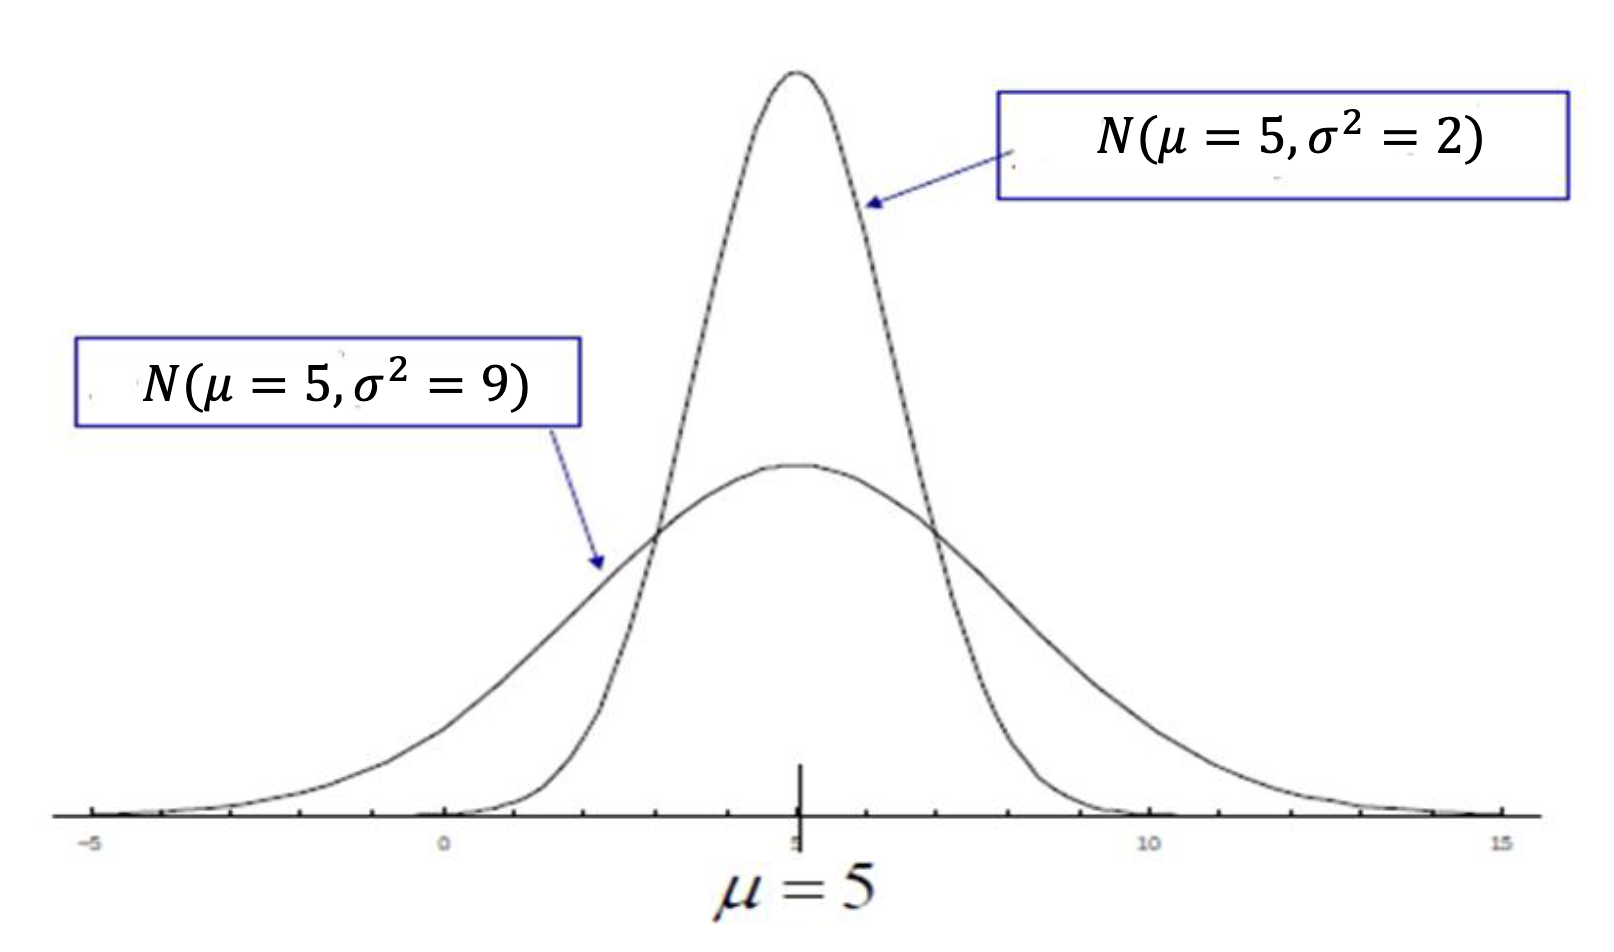
\includegraphics[width=1\linewidth]{img/effect-of-var.png}
      \caption{Effect of $\sigma^2$.}
    \end{minipage}
 \end{figure}

 \pagebreak

 \begin{note}
    \phantom{}\
    \begin{itemize}
        \item The mean shifts the distribution horizontally (shifts to the right as $\mu$ increases).
        \item The variance stretches the distribution (gets thicker and lower as $\sigma^2$ increases). 
    \end{itemize}
 \end{note}

 \begin{example}
    Heights or weights of males (or females) in large populations tend to follow a Normal distribution.
 \end{example}

 \textbf{The C.D.F.} of $N(\mu,\sigma^2)$ is
 \[
    F(x) = \int_{-\infty}^{x} \frac{1}{\sqrt{2\pi\sigma}} e^{-\frac{1}{2}\left(\frac{y-\mu}{\sigma}\right)^2} \, dy \quad x \in \R.
\]

\begin{note}
    Numerical methods are used to compute its value. 
\end{note}

$N(0,1)$ is called the ``\textbf{standard}'' Normal distribution with $\mu = 0$ and $\sigma = 1$. We have a ``new'' random variable $Z = \dis \frac{X - \mu}{\sigma}$, which is distributed as $Z \sim \text{N}(0,1)$.

\begin{theorem}
    Let $X \sim \text{N}(\mu,\sigma^2)$ and defined $Z = \dis \frac{X - \mu}{\sigma}$. Then $Z \sim \text{N}(0,1)$ and
    \[
        P(X \leq x) = P \left( Z \leq \frac{X - \mu}{\sigma} \right).
    \]
\end{theorem}

\begin{note}
    If we can compute the c.d.f. for $N(0,1)$, then we can compute it for other $N(\mu,\sigma^2)$ as well.
\end{note}

\textbf{What is this transformation doing?}

Consider the distribution of heights of young women aged 18 to 24. The distribution is approximately Normal with mean 64.5 inches and standard deviation 2.5 inches. We have $X \sim \text{N}(64.5,2.5^2)$.

\begin{figure}[htbp]
    \center
    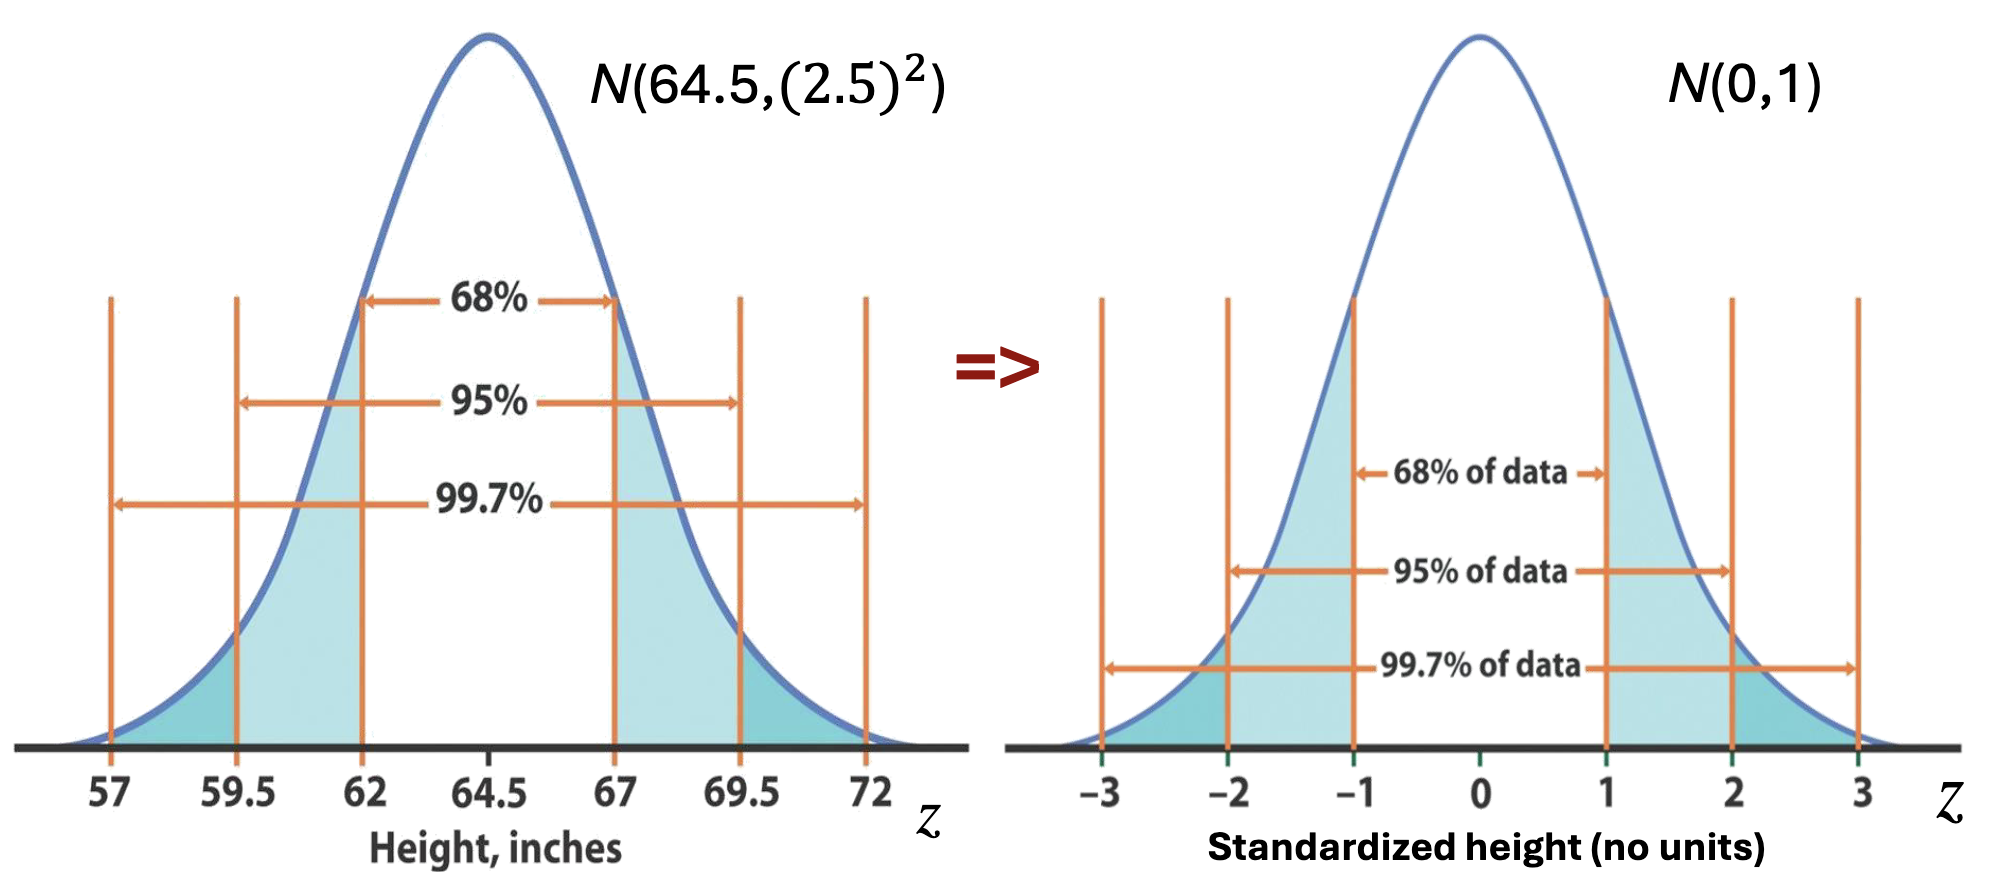
\includegraphics[scale=0.3]{img/Z-distribution.png}
    \caption{Transform to the standard Normal distribution.}
\end{figure}

\begin{theorem}[\textbf{Other Properties of Normal Distribution}]
    \phantom{}\\
    If $X \sim \text{N}(\mu,\sigma^2)$, then we have
    \begin{itemize}
        \item Symmetric about the mean: \vspace{-3mm}
        \[
            P(X \leq \mu - t) = P(X \geq \mu + t)
        \]
        or
        \[
            P(X \leq \mu + t) = P(X \geq \mu - t).
        \]
        \item Density is unimodal: peak is at $\mu$. Furthermore, mean and median also at $x = \mu$.
    \end{itemize}
\end{theorem}

\begin{figure}[htbp]
    \center
    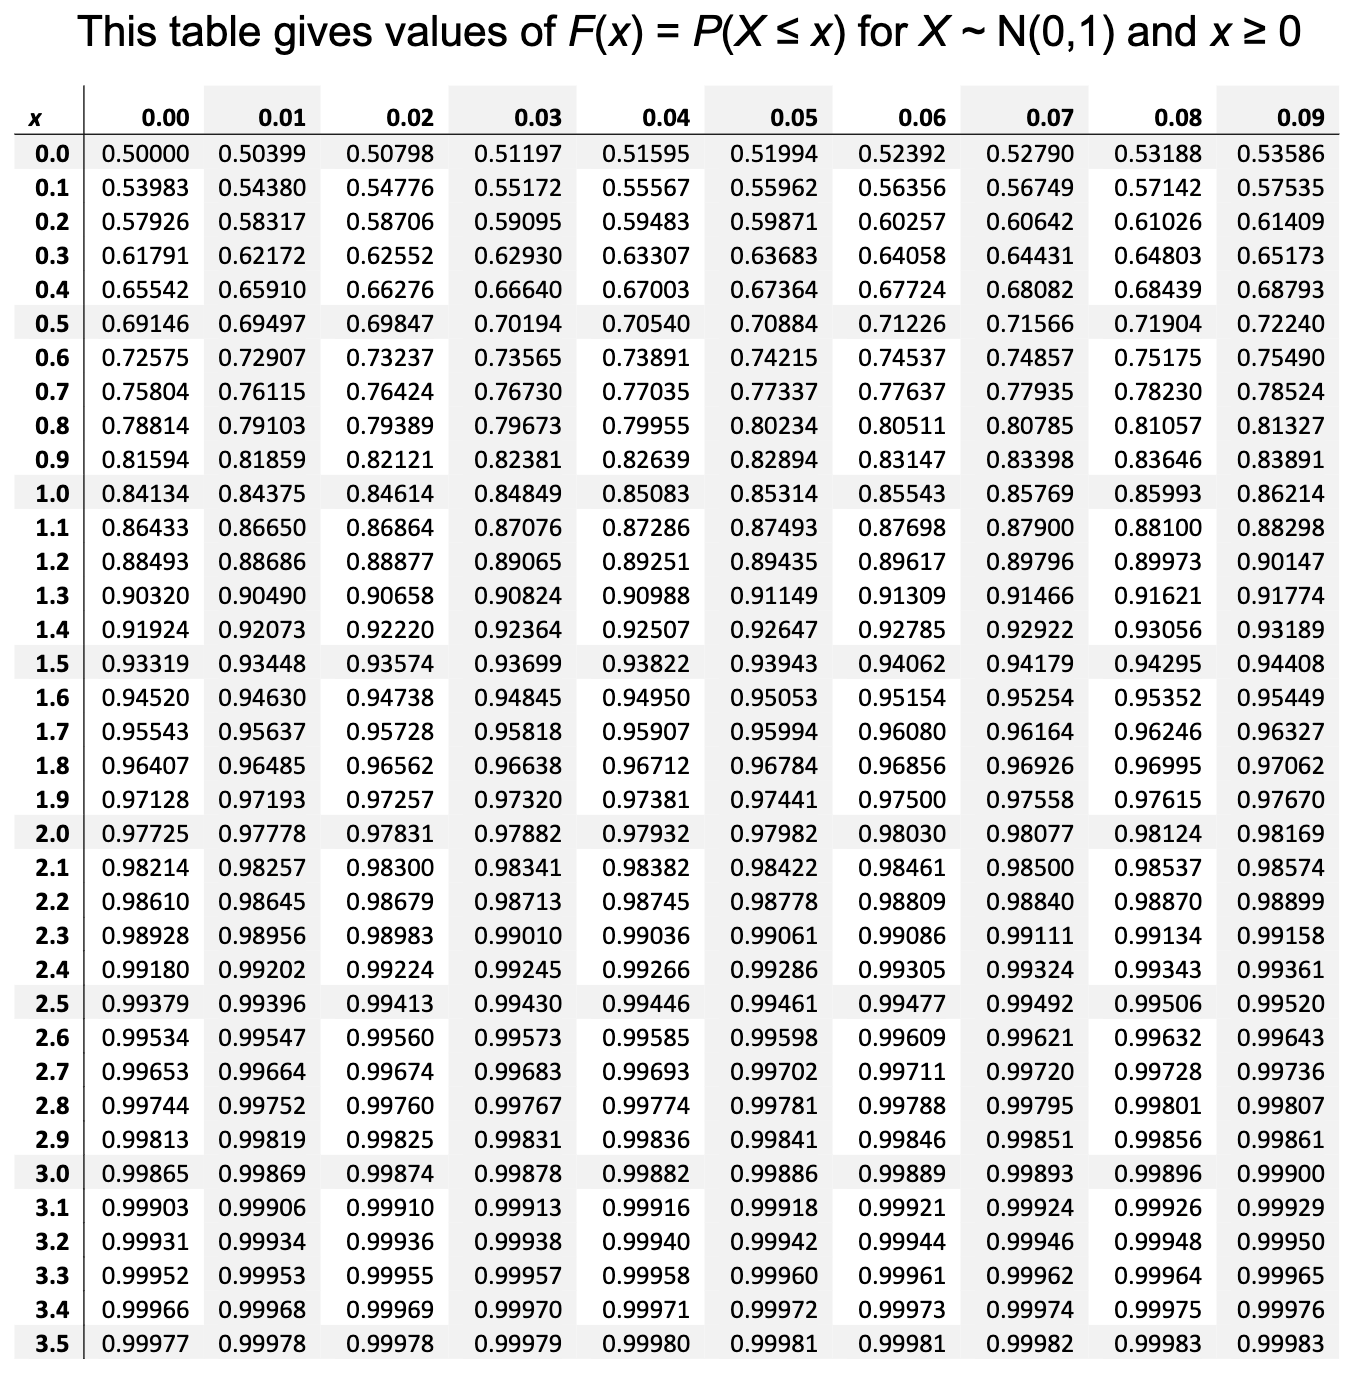
\includegraphics[scale=0.55]{img/N-CDF-table.png}
    \caption{Standard Normal Distribution c.d.f. values.}
\end{figure}

\textbf{How do we use the c.d.f. table?}

\begin{figure}[htbp]
    \center
    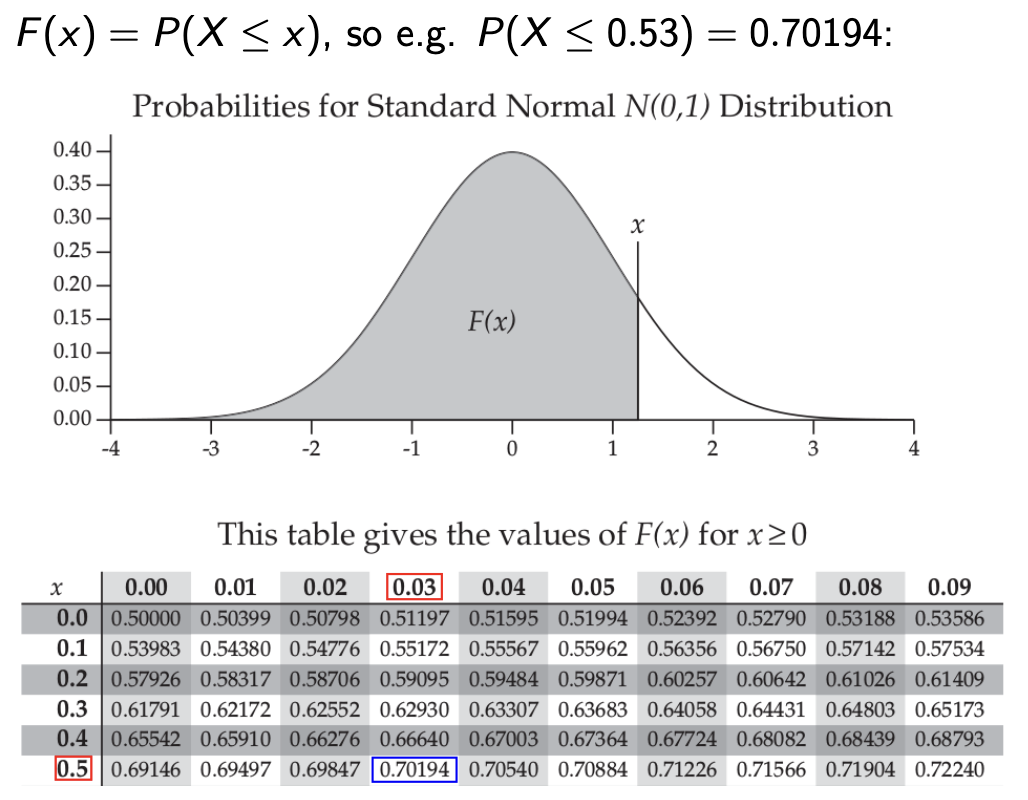
\includegraphics[scale=0.6]{img/N-table-example.png}
    \caption{Example of using the c.d.f. table.}
\end{figure}


\begin{example}
    Find a number $b$ such that $P(|Z| \leq b) = 0.95$. 

    \textbf{Solution:} Note that $P(|Z| \leq b) = P(-b \leq Z \leq b) = 0.95$. By symmetry, the probability outside $(-b,b)$ must be 0.05.

    $\implies P(Z \leq -b) + P(Z \geq b) = 0.05$. Furthermore, $P(Z \leq -b) = P(Z \geq b) = 0.025$ by symmetry again.

    $\implies P(Z \leq b) = 0.025 + 0.95 = 0.975.$ Looking for the value in the table, we get $b = 1.96$.
\end{example}

\begin{remark}
    Drawing out the normal distribution helps a lot!!!!! \\
\end{remark}

\textbf{Gaussian Distribution:} Another name for the Normal distribution. $X \sim \text{G}(\mu, \sigma)$ means that $X$ has  Gaussian distribution with mean $\mu$ and standard deviation $\sigma$. 

\begin{example}
    We can write $X \sim \text{N}(1,4)$ as $X \sim \text{G}(1,2)$.
\end{example}

\pagebreak

\begin{theorem}[\textbf{Standardization}]
    \[
        P(X \leq x) = P(\frac{X - \mu}{\sigma} \leq \frac{x - \mu}{\sigma}) = P(Z \leq \frac{x - \mu}{\sigma}),
    \]
    where $Z \sim \text{N}(0,1)$.
\end{theorem}

\begin{remark}
    Standardization can also be used for calculating other types of probabilities:
    \begin{itemize}
        \item $P(X > x) = P(Z > \frac{x - \mu}{\sigma})$.
        \item $P(a < X < b) = P(\frac{a - \mu}{\sigma} < Z < \frac{b - \mu}{\sigma}) = P(Z < \frac{b - \mu}{\sigma}) - P(Z < \frac{a - \mu}{\sigma})$. \\
    \end{itemize}
\end{remark}

\begin{example}
    Suppose $X \sim \text{N}(10,2)$, find $P(|X-10| \leq 3)$.

    \textbf{Solution:} 
    \begin{align*}
        P(|X-10| \leq 3) &= P(-3 \leq X - 10 \leq 3) \\
        &= P(7 \leq X \leq 13) \\
        &= P(\frac{7 - 10}{\sqrt{2}} \leq \frac{X - \mu}{\sigma} \leq \frac{13 - 10}{\sqrt{2}}) \quad \text{(standardize)} \\
        &= P(-2.12 \leq Z \leq 2.12) \\
        &= P(Z \leq 2.12) - P(Z \leq -2.12) \\
        &= P(Z \leq 2.12) - P(Z \geq 2.12) \\
        &= P(Z \leq 2.12) - \left[ 1 - P(Z \leq 2.12) \right] \\
        &= 2P(Z \leq 2.12) - 1 \\
        &= (2 \times 0.983) - 1 = 0.966.
    \end{align*}
\end{example}

\begin{example}[\textbf{Exercise}]
    Suppose $X \sim \text{N}(-7,14)$, find $P(|X+7| \geq 8)$. \\
    \textbf{Ans: $2 - 2P(Z \leq 2.14) = 0.03236$}.
\end{example}

\pagebreak

\begin{example}
    Suppose a certain mechanical component produced by a company has a width that is normally distributed with a mean $\mu = 2600$ and a standard deviation $\sigma = 0.6$.
    \begin{enumerate}[label=(\alph*)]
        \item What proportion of the components have a width outside the range 2599 to 2601?
        \item If the company needs to be able to guarantee to its purchaser that no more than 1 in 1000 of the
        components have a width outside the range 2599 to 2601, by how much does the value of $\sigma$ need to be reduced?
    \end{enumerate}

    \textbf{Solution:} 
    \begin{enumerate}[label=(\alph*)]
        \item Let $X = $ the width of a component. Then $X \sim \text{N}(2600,0.6^2)$. \vspace{-2mm}
        \begin{align*}
            P(X > 2601) + P(X < 2599) &= P(Z > \frac{2601 - 2600}{0.6}) + P(Z < \frac{2599 - 2600}{0.6}) \\
            &= P(Z > 1.67) + P(Z < -1.67) \quad \text{(standardize)} \\
            &= \left[ 1 - P(Z \leq 1.67) \right] + \left[ 1 - P(Z \leq 1.67) \right] \\
            &= 2 - 2P(Z \leq 1.67) \\
            &= 2 - (2 \times 0.95254) = 0.095.
        \end{align*}
        \item \phantom{} \vspace{-2mm}
        \begin{align*}
            P(X > 2601) + P(X < 2699) &\leq 0.001 \\
            1 - P(2599 < X < 2601) &\leq 0.001 \\
            P(2599 < X < 2601) &\geq 0.999 \\
            P(\frac{2599-2600}{\sigma} < Z < \frac{2601 - 2600}{\sigma}) &\geq 0.999 \\
            P(-\frac{1}{\sigma} < Z < \frac{1}{\sigma}) &\geq 0.999
        \end{align*}
        Using a sketch of the normal distribution, the probability within $(-\frac{1}{\sigma},\frac{1}{\sigma})$ $\geq$ 0.999. This means that we have probability $\leq$ 0.0005 at each side of the distribution. \\
        $\implies P(Z \leq \frac{1}{\sigma}) \geq 0.9995$ So, $\frac{1}{\sigma} = 3.29$.

        Therefore, we must have $\sigma \leq 0.30395$, need to reduce $\sigma$ by about 0.29605.
    \end{enumerate}
\end{example}

\pagebreak

\begin{figure}[htbp]
    \center
    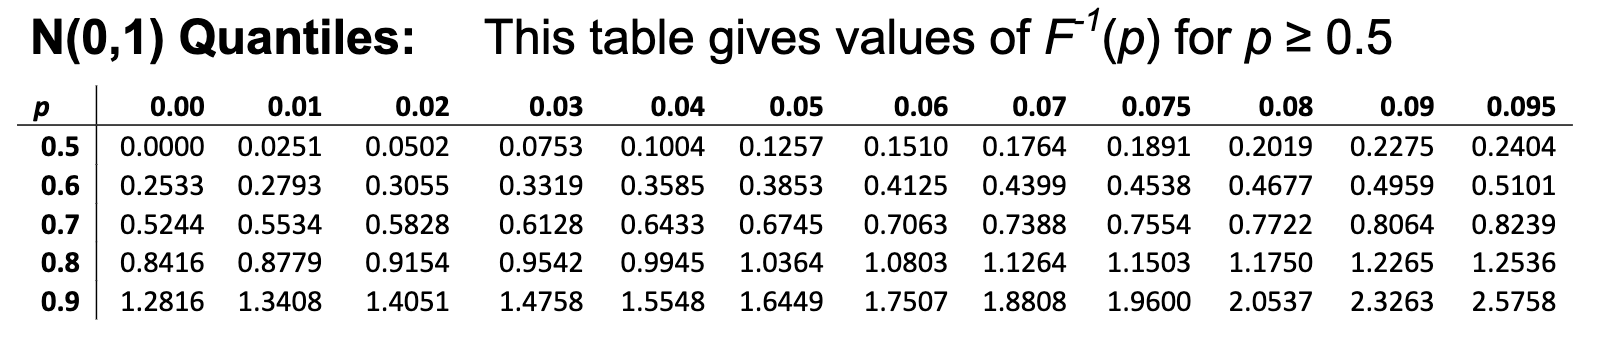
\includegraphics[scale=0.55]{img/quantiles-normal.png}
    \caption{Standard Normal Distribution Quantiles.}
\end{figure}

\begin{example}
    Let $X \sim \text{N}(0.28,0.05^2)$. Find the 90th quantile.

    \textbf{Solution:} $F^{-1}(0.9) = 1.2816 = Z$. Since $\dis Z = \frac{X-0.28}{0.05}$, we have $X = 0.344$. 
\end{example}

\newpage

\section{Multivariate Distributions}
\subsection{Basic Terminology and Techniques}

% An example of joint probability function table...
% \[
%     \begin{array}{cc|ccc|c}
%         & & \multicolumn{3}{c|}{x} & \\
%         \multicolumn{2}{c|}{f(x,y)} & 0 & 1 & 2 & \\
%         \hline
%         y & 1 & 0.1 & 0.2 & 0.3 & \\
%           & 2 & 0.2 & 0.1 & 0.1 & \\
%         \hline
%         & & & & & 1
%     \end{array}
% \]



\begin{definition}[\textbf{Joint Probability Function}]
    \phantom{}\\
    Let $X$ and $Y$ be two discrete random variables, we define the \textbf{joint probability function}
    $f(x, y)$ of $(X, Y)$ as \vspace{-3mm}
    \begin{align*}
        f(x, y) &= P(X = x \; \text{and} \; Y = y)    \\
                &= P(X = x, Y = y)
    \end{align*}
\end{definition}

\begin{remark}
    In general, if there are $n$ discrete random variables $X_1, X_2, \ldots, X_n$, we have \vspace{-2mm}
    \[f(x_1, x_2, \ldots, x_n) = P(X_1 = x_1, X_2 = x_2, \ldots, X_n = x_n).\]
\end{remark}


\begin{theorem}[\textbf{Properties of Joint Probability Function}]
    \phantom{}\
    \begin{itemize}
        \item $f(x, y) > 0 \; \forall (x, y)$.
        \item $\dis \sum_{\text{all } (x, y)} f(x, y) = 1$.
    \end{itemize}
\end{theorem}


\begin{example}
    Let $X$ be the number of daily purchases of a luxury item from a factory outlet location and Y be the daily number of purchases made online. Let 1,2, and 3 denote the number of purchases less than five, at least five but less than 15, and 15 or more respectively. The joint pf of X and Y is
    \[
        \begin{array}{cc|ccc|c}
            & & \multicolumn{3}{c|}{x} & \\
            \multicolumn{2}{c|}{f(x,y)} & 1 & 2 & 3 & \\
            \hline
            \multirow{3}{*}{y} 
              & 1 & 0.09 & 0.12 & 0.13 & \\
              & 2 & 0.12 & 0.11 & 0.11 & \\
              & 3 & 0.13 & 0.10 & 0.09 & \\
            \hline
            & & & & & 1
        \end{array}
    \]

    Find $f(1,2)$ and $f(2,2)$.

    \textbf{Solution:} $f(1,2) = P(X=1, Y=2) = 0.12$ and $f(2,2) = P(X=2, Y=2) = 0.11$.
\end{example}

\pagebreak

\textbf{What if we are only interested in \underline{one} of the variables?}

\begin{example}[continued]
    Say, we are only interested in $X$. Then, \vspace{-3mm}
    \begin{align*}
        P(X = 1) = P(B) &= P(B \cap A_1) + P(B \cap A_2) + P(B \cap A_3) \\
        & = P(X=1,Y=1) + P(X=1,Y=2) + P(X=1,Y=3) \\
        & = 0.34.
    \end{align*}
    Similarly, $P(X=2) = 0.33$ and $P(X = 3) = 0.33$.
\end{example}

\begin{note}
    \phantom{}\
    \begin{itemize}
        \item $\displaystyle \sum_{\text{all } x} f_X(x) = \displaystyle \sum_{\text{all } y} f_Y(y) = \displaystyle \sum_{\text{all } (x,y)} f_{X,Y}(x,y) = 1$.
    \end{itemize}
\end{note}


\begin{definition}[\textbf{Marginal Distributions}]
    \phantom{}\\
    Given the joint probability function of $X$ and $Y$, the \textbf{marginal distributions} are give by
    \begin{itemize}
        \item $f_1(x) = f_X(x) = \displaystyle \sum_{\text{all } y} f(x,y)$, with $x$ fixed.
        \item  $f_2(y) = f_Y(y) = \displaystyle \sum_{\text{all } x} f(x,y)$, with $y$ fixed.
    \end{itemize}
\end{definition}

\begin{remark}
    This idea can be extended beyond two variables.
\end{remark}

\begin{definition}[\textbf{Independent Random Variables}]
    \phantom{}\\
    $X$ and $Y$ are \textbf{independent} random variables $\iff$ $f(x, y) = f_1(x)f_2(y)$,
    $\forall$ $(x, y)$.
\end{definition}

In general, $X_1, X_2, \ldots, X_n$ are independent variables \vspace{-3mm}
    \[\iff f(x_1, x_2, \ldots, x_n) = f_1(x_1)f_2(x_2) \cdots f_n(x_n) \quad \forall x_1, x_2, \ldots, x_n.\]

\begin{remark}
    You can only conclude that $X$ and $Y$ are independent after checking \underline{ALL} $(x,y)$ combinations.
\end{remark}

\pagebreak

\begin{definition}[\textbf{Conditional Probability Function}]
    \phantom{}  \\
    The conditional probability function of $X$ given $Y = y$ is
    \[f_1(x|y) = \frac{f(x, y)}{f_2(y)} \quad \text{provided $f_2(y) > 0$}.\]
    Similarly, the conditional probability function of $Y$ given $X = x$ is
    \[f_2(y|x) = \frac{f(x, y)}{f_1(x)} \quad \text{provided $f_1(x) > 0$}.\]
\end{definition}

\begin{note}
    \phantom{}
    \begin{itemize}
        \item $f_1(x) = f_X(x)$ and $f_2(y) = f_Y(y)$.
        \item $\displaystyle \sum_{\text{all } x} f(x|y) = 1$.
    \end{itemize}
\end{note}

\begin{example}
    Continuing with our example:
    \[
        \begin{array}{cc|ccc|c}
            & & \multicolumn{3}{c|}{x} & \\
            \multicolumn{2}{c|}{f(x,y)} & 1 & 2 & 3 & f_Y(y) \\
            \hline
            \multirow{3}{*}{y} 
              & 1 & 0.09 & 0.12 & 0.13 & 0.34 \\
              & 2 & 0.12 & 0.11 & 0.11 & 0.34 \\
              & 3 & 0.13 & 0.10 & 0.09 & 0.32 \\
            \hline
            \multicolumn{2}{c|}{f_X(x)} & 0.34 & 0.33 & 0.33 & 1
        \end{array}
    \]
    Find the conditional probability function of $X$ given $Y = 1$, i.e find $f(x|1)$.

    \textbf{Solution:} Since $f(x|1) = \frac{f(x,1)}{f_Y(1)}$, we have \vspace{-2mm}
    \[
        \begin{array}{c|ccc|c}
            x & 1 & 2 & 3 & \text{Total} \\
            \hline
            f(x|1) & \frac{0.09}{0.34} = 0.26 & \frac{0.12}{0.34} = 0.35 & \frac{0.13}{0.34} = 0.38 & 1 \\
        \end{array}
    \]  
\end{example}

\begin{remark}
    If $X$ and $Y$ are independent, then $f(x|y) = \frac{f_1(x) f_2(y)}{f_2(y)} = f_1(x)$.
\end{remark}

\pagebreak

\textbf{Functions of Random Variables}

\begin{example}
    Let $U = Y - X$, where $X$ and $Y$ have the joint probability function given below. We might now be interested in finding the probability function of $U$, which is a function of $X$ and $Y$.
    \[
        \begin{array}{cc|ccc|c}
            & & \multicolumn{3}{c|}{x} & \\
            \multicolumn{2}{c|}{f(x,y)} & 1 & 2 & 3 & f_Y(y) \\
            \hline
            \multirow{3}{*}{y} 
              & 1 & 0.09 & 0.12 & 0.13 & 0.34 \\
              & 2 & 0.12 & 0.11 & 0.11 & 0.34 \\
              & 3 & 0.13 & 0.10 & 0.09 & 0.32 \\
            \hline
            \multicolumn{2}{c|}{f_X(x)} & 0.34 & 0.33 & 0.33 & 1
        \end{array}
    \]
    The possible values of $U$ are seen by looking at the value of $u = y - x$ for each $(x,y)$ in the range of $(X,Y)$.
    \[
        \begin{array}{cc|ccc}
            & & \multicolumn{3}{c}{x}  \\
            \multicolumn{2}{c|}{u}
            & 1 & 2 & 3 \\
            \hline
            \multirow{3}{*}{y}
            & 1 & 0 & -1 & -2 \\
            & 2 & 1 & 0 & -1 \\
            & 3 & 2 & 1 & 0
        \end{array}
    \]
    $P(U = 0) = P(X=1,Y=1) + P(X=2,Y=2) + P(X=3,Y=3) = 0.09 + 0.11 + 0.09 = 0.29$. Similarly for other values of $U$.
\end{example}

Let $T = X + Y$. Notice that to find $P(T=t)$, we are simply adding the probabilities for all $(x,y)$ combinations such that $x + y = t$. This could be written as:
\[
    f_T(t) = P(T=t) = \sum_{\substack{\text{all } (x, y) \\ \text{with } x + y = t}} f(x,y).
\]
However, if $x+y = t$, then $y = t - x$, so we have:
\[
    f_T(t) = P(T=t) = \sum_{\substack{\text{all } x}} f(x,y) = \sum_{\substack{\text{all } x}} P(X=x,Y=t-x).
\]

\pagebreak


In general, to find the probability function for $U = g(X,Y)$ of two random variables $X$ and $Y$, we have
\[
    f_U(u) = P(U = u) = \sum_{\substack{\text{all } (x, y) \\ \text{with } g(x,y)=u}} f(x,y).
\]

This can also be extended to functions beyond two random variables. \\

\begin{theorem}
    \phantom{}\\
    If $X \sim \text{Poisson}(\mu_1)$ and $Y \sim \text{Poisson}(\mu_2)$ are independent, then 
    $T = X + Y \sim \text{Poisson}(\mu_1 + \mu_2)$.
\end{theorem}


\begin{theorem}
    \phantom{}\\
    If $X \sim \text{Binomial}(n, p)$ and $Y \sim \text{Binomial}(m, p)$ are independent, then \\
    $T = X + Y \sim \text{Binomial}(n + m, p)$.
\end{theorem}
\phantom{}

\begin{example}
    In an auto parts company, an average of $\mu$ defective parts are produced per shift. The number, $X$, of defective parts produced has a Poisson distribution.
    An inspector checks all parts prior to shipping them, but there is a 10\% chance that a defective part will slip by undetected.

    Let $Y$ be the number of defective parts the inspector finds on a shift. Find $f(x|y)$.

    i.e. The company wants to know how many defective parts are produced, but can only know the number which are actually detected.

    \textbf{Solution:} The author was also studying for Actsc 231, so did not have enough time to bother writing out the entire solution. But if you work really hard, you'll have a chance to get:
    \[
        f(x|y) = \frac{e^{-\mu (1-p)} (\mu (1-p))^{x-y}}{(x-y)!} \quad \text{for x = y, y+1, \ldots}
    \]
\end{example}

\pagebreak

\subsection{Mutinomial Distribution}

This is a generalization of the Binomial to the case where each trial has $k$ possible outcomes.

\textbf{Physical Setup:} Similar to Binomial, except that now we have $\mathbf{k}$ types of outcomes. The experiment is repeated \textbf{independently} $\mathbf{n}$ times whith $\mathbf{k}$ \textbf{distinct outcomes} each time.

Let the probabilities of these $\mathbf{k}$ types be $\mathbf{p_1,p_2,\ldots,p_k}$ each time. Let $\mathbf{X_1} = \#$ of times the $1^{\text{st}}$ type occurs, \dots \, , $\mathbf{X_k} = \#$ of times the $k^{th}$ type occurs. Then $\left( X_1,X_2,\ldots,X_k \right)$ has a Multinomial distribution.

\begin{note}
    \phantom{}
    \begin{enumerate}
        \item $p_1 + p_2 + \cdots + p_k = 1$.
        \item $X_1 + X_2 + \cdots + X_k = n$. \\
        If we wish to drop one of the variables (say $X_k$), we note that \vspace{-3mm}
        \[
            X_k = n - X_1 - X_2 - \cdots - X_{k-1}.
        \]
    \end{enumerate}
\end{note}

\begin{example}
    A certain city has 3 television stations. During prime time on Saturday nights, Channel 12 has 50\% of the viewing audience, Channel 10 has 30\% and Channel 3 has 20\%.

    Let $X_1 = \#$ of families among $n$ watching channel 12, $X_2 = \ldots$ channel 10, and $X_3 = \ldots$ channel 3. Then $X_1,X_2,X_3 \sim \text{Multi}(n,p_1 = 0.5,p_2 = 0.3,p_3 = 0.2)$. \\
\end{example}

\textbf{Joint Probability Function:}

There are $\dis \binom{n}{x_1} \binom{n-x_1}{x_2} \cdots \binom{n-x_1 - \cdots - x_{k-1}}{x_k} = \frac{n!}{x_1! x_2! \cdots x_k!}$ number of ways to arrange $x_1$ items \vspace{-3mm} \\ 
of the $1^{\text{st}}$ type, $x_2$ items of the $2^{\text{nd}}$ type, $\ldots$, $x_k$ items of the $k^{\text{th}}$ type with a total of $n$ trials.

Each of these arrangements has probability $p_1^{x_1}p_2^{x_2} \cdots p_k^{x_k}$ since $p_1$ is multiplied $x_1$ times in some order, etc, and trials are independent. Therefore,
\[
    f(x_1,\ldots ,x_k) = \frac{n!}{x_1! x_2! \cdots x_k!} p_1^{x_1}p_2^{x_2} \cdots p_k^{x_k}
\]
with $x_i = 0,1,\ldots ,n$ and $\displaystyle \sum_{i=1}^{k} x_i = n$.
Note that $\displaystyle \sum f(x_1,\ldots ,x_k) = 1$.

\pagebreak

\textbf{Marginal and Joint Probability Functions:}

If we are interested in finding the marginal distribution of one variable, $X_2$, in the multinomial distribution, we can:

\begin{enumerate}
    \item Mathematical approach: fix the value $x_2$ and then sum over all the other variables:
    \[
        f_2(x_2) = \displaystyle \sum_{\substack{\text{all }x_1,x_3,\ldots ,x_k}} f(x_1,\ldots ,x_k)
    \]
    for each $x_2 = 0,1,\ldots , n$. This is algebraically hard.

    \item Intuitive and simple approach: if we are only interested in $X_2$ (i.e. the $\#$ of occurrences of the second type among $n$ trials), we notice that
    \begin{itemize}
        \item The experiment is repreated $n$ times and $X_2 = 0,1,\ldots ,n$.
        \item The probability that this second event occurs on each trial is $p_2$ and the probability it doesn't occur is $1-p_2$.
        \item Each trial is assumed independent.
        \item Hence, $X_2 \sim \text{Binomial}(n,p_2)$ and $p_2 = 1 - (p_1 + p_3 + \cdots + p_k)$.
    \end{itemize}
\end{enumerate}

\textbf{What about $T = X_1 + X_2$?} \\
Using a similar argument, we could make our ``success'' =  an occurrence in one of the first two types, whereas anything else is considered a ``failure''.

Let $T = \#$ of type 1 or type 2 outcomes among $n$ trials. Then $T \sim \text{Binomial}(n,p_1 + p_2)$.
\begin{itemize}
    \item Two outcomes: type 1 \& 2 vs. anything else.
    \item Independent trials.
    \item Multiple trials: $n$.
    \item Same  $P(\text{success}) = P(\text{type 1} \cup \text{type 2}) = P(\text{type 1}) + P(\text{type 2}) = p_1 + p_2$.
\end{itemize}

\textbf{What about the conditional distribution of $X_1$ given $T = t$?} \\
$X_1 | T=t \sim \text{Bin}(t, \frac{p_1}{p_1 + p_2})$. So $f(x_1|t) = \binom{t}{x_1} \left( \frac{p_1}{p_1 + p_2} \right)^{x_1} \left( 1 - \frac{p_1}{p_1 + p_2} \right)^{t - x_1}$.


\pagebreak

\begin{example}
    The probabilities that a certain electronic component will last less than 50 hours in continuous use, between 50 and 90 hours, or more than 90 hours, are $p_1 = 0.2$, $p_2 = 0.5$, and $p_3 = 0.3$, respectively.

    The time to failure of eight such components is recorded. \\
    $X_1 = \#$ of components among 8 that fail in $< 50$ hours. \\
    $X_2 = \#$ of components among 8 that fail in $[50,90]$ hours. \\
    $X_3 = \#$ of components among 8 that fail in $> 90$ hours.
    \begin{enumerate}[label=(\alph*)]
        \item What is the probability that one will last less than 50 hours, five will last between 50 and 90 hours, and two will last more than 90 hours?
        \item What is the probability that at least 3 will last between 50 and 90 hours?
        \item What is the joint probability function of the number of components that last less than 50 hours and the number of components that last between 50 and 90 hours?
    \end{enumerate}

    \textbf{Solution:}
    \begin{enumerate}[label=(\alph*)]
        \item Mutinomial with $n=8$. $f(1,5,2) = P(X_1 = 1, X_2 = 5, X_3 = 2) = \frac{8!}{1!5!2!}(0.2)^1 (0.5)^5 (0.3)^2$.
        \item $X_2 \sim \text{Bin}(8,0.5)$. \vspace{-3mm}
        \begin{align*}
            P(X_2 \geq 3) &= 1 - P(X_2 \leq 2) \\
            &= 1 - \left[ P(X_2 = 0) + P(X_2 = 1) + P(X_2 = 2) \right] \\
            &= 1 - \left[ \binom{8}{0} (0.5)^0 (0.5)^8 + \binom{8}{1} (0.5)^1 (0.5)^7 + \binom{8}{2} (0.5)^2 (0.5)^6 \right]
        \end{align*}
        \item $X_1,X_2 \sim \text{Multinomial}(n=8,p_1=0.2,p_2=0.5,1-p_1 -p_2 = 0.3)$. \\
        Therefore, $f(x_1,x_2) = \frac{8!}{x_1! x_2! (8-x_1 - x_2)!}0.2^{x_1}0.5^{x_2} 0.3^{8-x_1-x_2}$. \\
    \end{enumerate}
\end{example}


\subsection{Markov Chains}

Not covered material.


\pagebreak


\subsection{Expectation for Multivariate Distributions: Covariance and Correlation}


Extending the definition of expected value to multiple discrete random variables.
\begin{definition}
    \[\expect{g(X,Y)} = \dis \sum_{\text{all } (x,y)} g(x,y)f(x,y)\] and
    \[\expect{g(X_1, X_2, \ldots, X_n)} = \sum_{\text{all } (x_1, x_2, \ldots, x_n)} g(x_1, x_2, \ldots, x_n)f(x_1, x_2, \ldots, x_n).\]
\end{definition}

\begin{example}
    Let the joint probability function $f(x,y)$ be given be the following table:
    \[
        \begin{array}{cc|ccc|c}
            & & \multicolumn{3}{c|}{x} & \\
            \multicolumn{2}{c|}{f(x,y)} & 0 & 1 & 2 & f_Y(y) \\
            \hline
            \multirow{2}{*}{y} 
              & 1 & 0.1 & 0.2 & 0.3 & 0.6 \\
              & 2 & 0.2 & 0.1 & 0.1 & 0.4 \\
            \hline
            \multicolumn{2}{c|}{f_X(x)} & 0.3 & 0.3 & 0.4 & 1
        \end{array}
    \]
    Find $\expect{XY}$ and $\expect{X}$.

    \textbf{Solution:} Here we have $g(X,Y) = XY$. \vspace{-3mm}
    \begin{align*}
        \expect{XY} &= \dis \sum_{\text{all } (x,y)} xyf(x,y) \\
        &= (0 \times 1)(0.1) + (1 \times 1)(0.2) + (2 \times 1)(0.3) + (0 \times 2)(0.2) + (1 \times 2)(0.1) + (2 \times 2)(0.1) \\
        &= 1.4.
    \end{align*}
    \phantom{} \vspace{-2mm}
    For $\expect{X}$, we keep $x$ fixed and use $f_1(x)$: \vspace{-2mm}
    \begin{align*}
        \expect{X} &= \displaystyle \sum_{x=0}^{2} xf_1(x) \\
        &= (0 \times 0.3) + (1 \times 0.3) + (2 \times 0.4) \\
        &= 1.1.
    \end{align*}
\end{example}


\begin{theorem}[\textbf{Property of Multivariate Expectation}]
    \[\expect{ag_1(X, Y) + bg_2(X, Y)} = a\expect{g_1(X, Y)} + b\expect{g_2(X, Y)}.\]
(This can be extended beyond two functions and beyond two variables).
\end{theorem}

\textbf{Relationships between Variables}

\begin{definition}[\textbf{Covariance}]
    The \textbf{covariance} of $X$ and $Y$, denoted by $\Cov{X, Y}$ or $\sigma_{XY}$, is
    \[\Cov{X, Y} = \expect{(X - \mu_X)(Y - \mu_Y)}.\]
\end{definition}

\begin{note}
    \phantom{} \vspace{-3mm}
    \begin{align*}
        \Cov{X, Y} &= \expect{(X - \mu_X)(Y - \mu_Y)}   \\
                   &= \expect{XY - \mu_XY - X\mu_Y + \mu_X\mu_Y}    \\
                   &= \expect{XY} - \mu_X\expect{Y} - \mu_Y\expect{X} + \mu_X\mu_Y  \\
                   &= \expect{XY} - \expect{X}\expect{Y} - \expect{Y}\expect{X} + \expect{X}\expect{Y}  \\
                   &= \expect{XY} - \expect{X}\expect{Y}
    \end{align*}
    and we usually use $\Cov{X, Y} = \expect{XY} - \expect{X}\expect{Y}$ for calculations. 
\end{note}

\begin{example}
    Let the joint probability function $f(x,y)$ be given be the following table:
    \[
        \begin{array}{cc|ccc|c}
            & & \multicolumn{3}{c|}{x} & \\
            \multicolumn{2}{c|}{f(x,y)} & 0 & 1 & 2 & f_Y(y) \\
            \hline
            \multirow{2}{*}{y} 
              & 1 & 0.1 & 0.2 & 0.3 & 0.6 \\
              & 2 & 0.2 & 0.1 & 0.1 & 0.4 \\
            \hline
            \multicolumn{2}{c|}{f_X(x)} & 0.3 & 0.3 & 0.4 & 1
        \end{array}
    \]
    Find $\Cov{X,Y}$.

    \textbf{Solution:} From above example, we know that $\expect{XY} = 1.4$ and $\expect{X} = 1.1$. \\
    And $\expect{Y} = (1 \times 0.6) + (2 \times 0.4) = 1.4$. So $\Cov{X,Y} = 1.4 - (1.1 \times 1.4) = -0.14$ suggesting a negative relationship between $X$ and $Y$.
\end{example}

\textbf{Interpretation of Covariance}

\begin{figure}[htbp]
    \center
    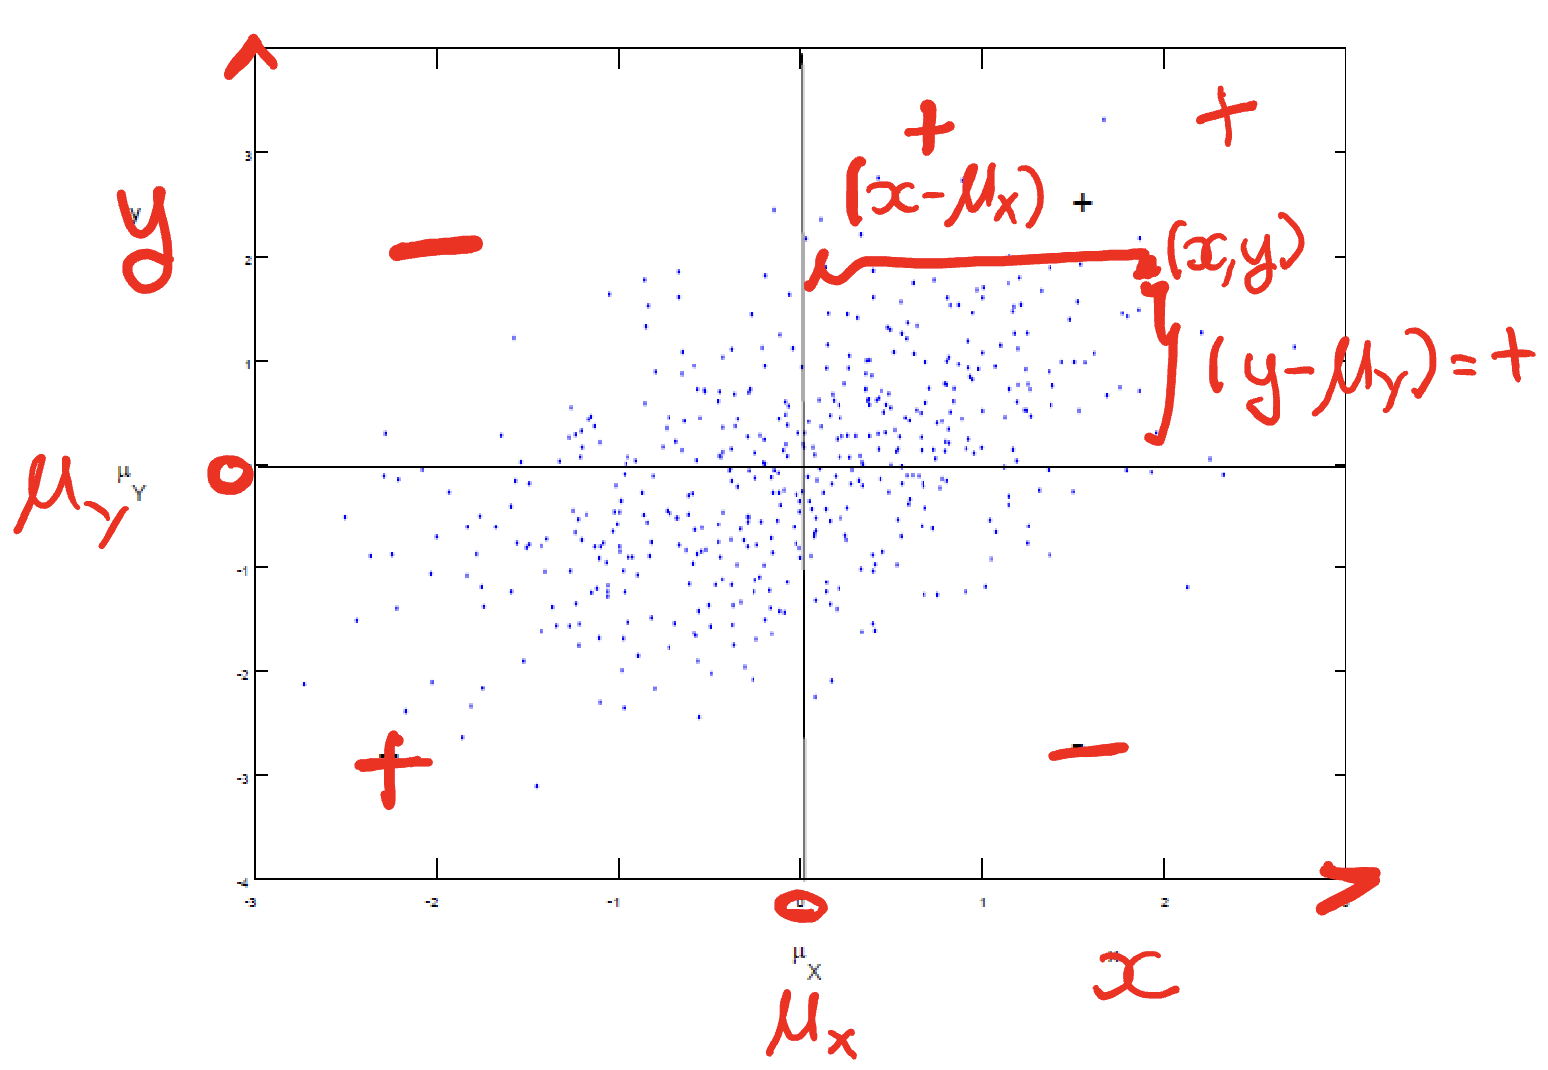
\includegraphics[scale=0.5]{img/cov.png}
    \caption{Random points $(X,Y)$ with $\Cov{X,Y} = 0.5$, variances 1.}
\end{figure}


\begin{theorem}
    If $X$ and $Y$ are independent then $\Cov{X, Y} = 0$.
\end{theorem}

\begin{note}
    The converse it NOT true.
\end{note}

% \begin{proof}
%     Recall that $\expect{X - \mu_X} = \expect{X} - \mu_X = 0$. Let $X$ and $Y$ be independent.  \\
%     Then $f(x, y) = f_1(x)f_2(y)$.
%     \begin{align*}
%         \Cov{X, Y} &= \expect{(X - \mu_X)(Y - \mu_Y)}   \\
%                    &= \sum_{\text{all } y} \left[\sum_{\text{all } x} (x - \mu_X)(y - \mu_Y)f_1(x)f_2(y)\right] \\
%                    &= \sum_{\text{all } y} \left[(y - \mu_Y)f_2(y)\sum_{\text{all } x} (x - \mu_X)f_1(x)\right] \\
%                    &= \sum_{\text{all } y} \left[(y - \mu_Y)f_2(y)\expect{X - \mu_X}\right] \\
%                    &= \sum_{\text{all } y} 0    \\
%                    &= 0.
%     \end{align*}
% \end{proof}
% This result can also be proved using the Theorem below.

\begin{theorem}
    Suppose $X$ and $Y$ are independent random variables. Then, if $g_1(X)$ and
    $g_2(Y)$ are two functions, we have
    \[\expect{g_1(X)g_2(Y)} = \expect{g_1(X)}\expect{g_2(Y)}.\]
\end{theorem}

\begin{note}
    $\expect{XY} = \displaystyle \sum_{\text{all $(x,y)$}} xyf(x,y) = \displaystyle \sum_{\text{all $x$}} \displaystyle \sum_{\text{all $y$}} xyf(x,y)$.
\end{note}

\pagebreak

\begin{definition}[\textbf{Correlation Coefficient}]
    The \textbf{correlation coefficient} of $X$ and $Y$ is
    \[\rho = \Corr{X,Y} = \frac{\Cov{X, Y}}{\sigma_X \sigma_Y}.\]    
\end{definition}

\begin{note}
    Alternatively, $\rho = \dis \frac{\Cov{X,Y}}{\sqrt{\Var{X} \Var{Y}}}$.
\end{note}

The correlation coefficient measures the strength of the \textbf{linear} relationship between $X$ and $Y$, it is essentially
a rescaled version of the covariance, scaled to lie in the interval $[-1, 1]$.




\begin{theorem}[\textbf{Properties of $\rho$}]
    \phantom{}\
    \begin{enumerate}
        \item Since $\sigma_X$, $\sigma_Y > 0$, $\rho$ will have the same sign as $\Cov{X,Y}$. Hence the interpretation of the sign of $\rho$ is the same as for $\Cov{X,Y}$, and $\rho = 0$ if $X$ and $Y$ are independent. When $\rho = 0$, we say that $X$ and $Y$ are uncorrelated.
        \item $-1 \leq \rho \leq 1$ and as $\rho \to \pm 1$ the relation between $X$ and $Y$ becomes one-to-one and linear.
    \end{enumerate}
\end{theorem}


\begin{example}
    The joint probability function of $(X,Y)$ is:
    \[
        \begin{array}{cc|ccc|c}
            & & \multicolumn{3}{c|}{x} & \\
            \multicolumn{2}{c|}{f(x,y)} & 0 & 1 & 2 & f_Y(y) \\
            \hline
            \multirow{2}{*}{y} 
              & 0 & 0.06 & 0.15 & 0.09 & 0.3 \\
              & 1 & 0.14 & 0.35 & 0.21 & 0.7 \\
            \hline
            \multicolumn{2}{c|}{f_X(x)} & 0.2 & 0.5 & 0.3 & 1
        \end{array}
    \]
    Calculate the correlation coefficient. What does this say about the relationship between $X$ and $Y$?

    \textbf{Solution:} $\expect{Y} = (1 \times 0.7) = 0.7$, $\expect{X} = (1 \times 0.5) + (2 \times 0.3) = 1.1$, $\expect{XY} = (1 \times 1 \times 0.35) + (2 \times 1 \times 0.21) = 0.77$. 

    $\implies \Cov{X,Y} = 0.77 - (0.7 \times 1.1) = 0$. So $\rho = \Corr{X,Y} = \frac{0}{\sigma_X \sigma_Y} = 0$. \\
    Therefore, $X$ and $Y$ have no linear association (and in fact, $X$ and $Y$ are independent, we can show this for all $(x,y)$).
\end{example}

\subsection{Mean and Variance of a Linear Combination of Random Variables}

\begin{theorem}[\textbf{Results for Expectations}]
    \phantom{}
    \begin{enumerate}
        \item $\expect{aX+bY} = a\expect{X} + b\expect{Y}$.
        \item Let $a_i$ be constants and $\expect{X_i} = \mu_i$, $i = 1,2,\ldots ,n$. Then $\expect{\displaystyle \sum_{i=1}^{n} a_iX_i} = \displaystyle \sum_{i=1}^{n} a_i \mu_i$. In particular, $\expect{\displaystyle \sum_{i=1}^{n} X_i}  = \displaystyle \sum_{i=1}^{n} \expect{X_i}$. \vspace{1mm}
        \item Let $X_1, X_2,\ldots , X_n$ be random variables which have mean $\mu$. Then, the sample mean is $\overline{X} = \dis \frac{\displaystyle \sum_{i=1}^{n} X_i}{n}$ and $\expect{\overline{X}} = \mu$. 
    \end{enumerate}
\end{theorem}

\begin{theorem}[\textbf{Results for Covariance}]
    \phantom{}
    \begin{enumerate}
        \item $\Cov{X,X} = \Var{X}$.
        \item $\Cov{aX+bY,cU+dV} = ac\Cov{X,U} + ad\Cov{X,V} \\ \hspace*{40mm}+ bc\Cov{Y,U} + bd\Cov{Y,V}$.
    \end{enumerate}
\end{theorem}
\begin{note}
    Covariance is symmetric: $\Cov{X,Y} = \Cov{Y,X}$. And for all $c\in \R$, $\Cov{c,X} = 0$.
\end{note}

\begin{theorem}[\textbf{Results for Variance}]
    \phantom{}
    \begin{enumerate}
        \item \textbf{Variance of a linear comobination:} \vspace{-3mm}
        \[
            \Var{aX+bY} = a^2\Var{X} + b^2\Var{Y} + 2ab\Cov{X,Y}.
        \]
        \item \textbf{Variance of a sum of independent random variables:} \\
        Let $X$ and $Y$ be independent. Since $\Cov{X,Y} = 0$, result 1 gives \vspace{-3mm}
        \[
            \Var{X+Y} = \Var{X} + \Var{Y} = \Var{X-Y}.
        \]
        \item \textbf{Variance of a general linear combination of random variables:} \\
        Let $a_i$ be constants. Then \vspace{-3mm}
        \[
            \Var{\displaystyle \sum_{i=1}^{n} a_iX_i} = \displaystyle \sum_{i=1}^{n} a_i^2\Var{X_i} + 2\displaystyle \sum_{i=1}^{n} \sum_{j=i+1}^{n} a_i a_j \Cov{X_i,X_j}. 
        \]
        \pagebreak
        \item \textbf{Variance of a linear combination of independent random variables:} \\
        Special cases of result 3 are:
        \begin{enumerate}
            \item If $X_1, X_2, \ldots, X_n$ are independent, then $\Cov{X_i,X_j} = 0$, so that \vspace{-3mm}
            \[
                \Var{\displaystyle \sum_{i=1}^{n} a_iX_i} = \displaystyle \sum_{i=1}^{n} a_i^2\Var{X_i}.
            \]
            \item If $X_1, X_2, \ldots, X_n$ are independent and all have the same variance $\Var{X} = \sigma^2$, then \vspace{-3mm}
            \[
                Var{\left( \overline{X} \right)} = \frac{\sigma^2}{n}.
            \]
        \end{enumerate}
    \end{enumerate}
\end{theorem}

\begin{remark}
    If $X_1,X_2,\ldots ,X_n$ are independent random variables with the same mean $\mu$ and the same variance $\sigma^2$, then the sample mean $\overline{X} = \frac{1}{n}\displaystyle \sum_{i=1}^{n} X_i$ has \vspace{-3mm}
    \[
        \expect{\overline{X}} = \mu \quad \text{and} \quad \Var{\overline{X}} = \frac{\sigma^2}{n}.
    \]
    What does this tell us about $\overline{X}$? 
    
    $\implies \overline{X}$ is less variable than $X_i$ (the larger $n$ is the less variability there is).
    \begin{itemize}
        \item This happens because as n increases, we are adding more
        information and so our sample mean. $\overline{X}$ is becoming \textbf{more precise} in sense that we have \vspace{-3mm}
        \[
            \Var{\overline{X}} \to 0 \text{ as } n \to \infty.
        \]
        \item This implies that as $n\to \infty$, $\overline{X} \to \mu$.
        \item This is something called the ``\textbf{law of averages}''.
    \end{itemize}
\end{remark}

\pagebreak


\subsection{Linear Combinations of Independent Normal Random Variables}

\begin{theorem}[\textbf{Linear Combinations of Independent Normal Random Variables}]
    \phantom{}
    \begin{enumerate}
        \item Let $X \sim N(\mu, \sigma^2)$ and $Y = aX + b$, where $a$, $b \in \R$.
        Then, $Y \sim N(a\mu + b, a^2\sigma^2)$.
        \item Let $X \sim N(\mu_1, \sigma_1^2)$ and $Y \sim N(\mu_2, \sigma_2^2)$ be independent random variables, and let $a$ and $b$ be constants.
        Then, $aX+bY \sim \text{N}(a\mu_1 + b\mu_2, a^2\sigma_1^2 + b^2\sigma_2^2)$. \\
        In general, if $X_i \sim \text{N}(\mu_i, \sigma_i^2)$, $i=1,2,\ldots,n$, are independent random variables and $a_1,a_2,\ldots a_n \in \R$, then $\displaystyle \sum_{i=1}^{n} a_iX_i \sim \text{N}\left( \displaystyle \sum_{i=1}^{n} a_i\mu_i, \displaystyle \sum_{i=1}^{n} a_i^2 \sigma_i^2 \right)$.
        \item Let $X_1, X_2, \ldots, X_n$ be independent $N(\mu, \sigma^2)$ random variables. Then
        $\dis \sum_{i=1}^{n} X_i \sim N(n\mu, n\sigma^2)$ and $\overline{X} \sim N(\mu, \frac{\sigma^2}{n})$.
    \end{enumerate}
\end{theorem}

\begin{note}
    We have $\expect{aX+b} = a\mu + b$ and $\Var{aX+b} = a^2\sigma^2$. \\
\end{note}

\begin{example}
    Let $X \sim \text{N}(3,5)$ and $Y \sim \text{N}(6,14)$ be independent random variables. Find $P(X > Y)$.

    \textbf{Solution:} Note that $P(X > Y) = P(X - Y > 0)$. Let $W = X - Y$. Then $\expect{W} = \expect{X} - \expect{Y} = 3 - 6 = -3$ and $\Var{W} = \Var{X} + \Var{Y} = 5 + 14 = 19$ since $X$ and $Y$ are independent. So $W \sim \text{N}(-3,19)$. \vspace{-3mm}
    \begin{align*}
        P(X > Y) & = P(W > 0) \\
        &= P(Z > \frac{0-(-3)}{\sqrt{19}}) \\
        &= P(Z > 0.69) \\
        &= 1 - P(Z \leq 0.69) = 0.245.
    \end{align*}
\end{example}

\begin{example}
    Let $X \sim \text{N}(5,4)$. An independent random variable $Y$ is also normal with mean 7 and standard deviation of 3. Find:
    \begin{enumerate}[label=(\alph*)]
        \item The probability $2X$ differs from $Y$ by more than 4.
        \item The minimum number, $n$, of independent observations needed on $X$ so that $P(|\overline{X} -5| < 0.1) \geq 0.98$.
    \end{enumerate}
    \pagebreak

    \textbf{Solution:}
    \begin{enumerate}[label=(\alph*)]
        \item Let $W = 2X - Y$. Then $\expect{W} = 2\expect{X} - \expect{Y} = 10 - 7 = 3$ and $\Var{W} = 4\Var{X} + \Var{Y} = 16 + 3^2 = 25$. Next, \vspace{-3mm}
        \begin{align*}
            P(|2X - Y|> 4) = P(|W|>4) &= P(W>4) + P(W<-4) \\
            &= P(Z > \frac{4-3}{5}) + P(Z < \frac{-4-3}{5}) \\
            &= P(Z > 0.2) + P(Z < -1.4) \\
            &= \left[ 1 - P(Z \leq 0.2) \right] + \left[ 1 - P(Z \leq 1.4) \right]
        \end{align*}
        \item We have that $\overline{X} \sim \text{N}(\mu = 5, \frac{\sigma^2}{n} = \frac{4}{n})$. 
        \begin{align*}
            P(|\overline{X} -5| < 0.1) &\geq 0.98 \\
            P(-0.1 < \overline{X} - 5 < 0.1) &\geq 0.98 \\
            P(\frac{-0.1}{\sqrt{\frac{4}{n}}} < Z < \frac{0.1}{\sqrt{\frac{4}{n}}}) &\geq 0.98 \\
            \implies P(Z \leq \frac{0.1}{\sqrt{\frac{4}{n}}}) &\geq 0.99 \quad \text{use a graph...} \\
            \frac{0.1}{\sqrt{\frac{4}{n}}} &\geq 2.33 \implies n \geq 2171.56 \\
            n &= 2172.
        \end{align*}
        More precisely, use R to get $n \geq 2165$.
    \end{enumerate}
\end{example}


\pagebreak

\subsection{Indicator Random Variables}

An indicator variable is a binary variable (0 or 1) that indicates whether or not an event has occurred. It can allow us to take more complicated scenarios and break them into simpler ones.

\begin{example}
    Let $X \sim \text{Bin}(n,p)$. Define new random variables $X_i$ by \vspace{-3mm}
    \[
        X_i = 
        \begin{cases} 
            0 & \text{if $i^{\text{th}}$ trial was a failure} \\
            1 & \text{if $i^{\text{th}}$ trial was a success}
        \end{cases}.
    \]

    The random variable $X_i$ indicates whether `success' occured on the $i^\text{th}$ trial. The total number of successes is $X = \displaystyle \sum_{i=1}^{n} X_i$. We can find the mean and variance of $X_i$ and then use our results for mean and variance to find $\mu$ and $\sigma^2$ of $X$. First, \vspace{-3mm}
    \[
        \expect{X_i} = \displaystyle \sum_{x_i=0}^{1} x_i f(x_i) = 0f(0) + 1f(1) = f(1). 
    \]
    But $f(1) = p$ since $P(\text{success}) = p$ on each trial. Therefore $\expect{X_i} = p$. And since $X_i = 0$ or 1, so $X_i = X_i^2$, and therefore 
    \[
        \expect{X_i^2} = \expect{X_i} = p.
    \]
    Thus, 
    \[
        \Var{X_i} = \expect{X_i^2} - \left( \expect{X_i} \right)^2 = p - p^2 = p(1-p).
    \]
    In the Binomial distribution the trials are independent, so the $X_i$'s are also independent. Thus
    \begin{align*}
        \expect{X} &= \expect{\displaystyle \sum_{i=1}^{n} X_i} = \displaystyle \sum_{i=1}^{n} \expect{X_i} = \displaystyle \sum_{i=1}^{n} p = np. \\
        \Var{X} &= \Var{\displaystyle \sum_{i=1}^{n} X_i} = \displaystyle \sum_{i=1}^{n} \Var{X_i} = \displaystyle \sum_{i=1}^{n} p(1-p) = np(1-p).
    \end{align*}
\end{example}

\begin{remark}
    Note that $X_i \sim \text{Binomial}(1,p)$ is actually a Binomial random variable. In some problems the $X_i$'s are not independent, we will also need covariances.
\end{remark}


\pagebreak

\begin{example}
    We have $N$ letters to $N$ different people, and $N$ envelopes addressed to those $N$ people. One letter is put in each envelope at random. Find the mean and variance of the number of letters placed in the right envelopes.

    \textbf{Solution:}
    Let
    \[
        X_i = 
        \begin{cases} 
            0 & \text{if letter $i$ is not in envelope $i$} \\
            1 & \text{if letter $i$ is in envelope $i$}
        \end{cases}.
    \]

    Then, the total number of correctly placed letters is $\displaystyle \sum_{i=1}^{N} X_i$. Note that $X_i$'s are dependent since the experiment is done without replacenent!
    \[
        \expect{X_i} = \displaystyle \sum_{x_i=0}^{1} x_if(x_i) = f(1) = \frac{1}{N} = \expect{X_i^2}
    \]
    since there is 1 chance in $N$ that letter $i$ will be put in envelope $i$ and then,
    \[
        \Var{X_i} = \expect{X_i} - \left( \expect{X_i} \right)^2 = \frac{1}{N} - \frac{1}{N^2} = \frac{1}{N}\left( 1 - \frac{1}{N} \right).
    \]
    Therefore,
    \[
        \expect{\displaystyle \sum_{i=1}^{N} X_i} = \displaystyle \sum_{i=1}^{N} \expect{X_i} = \displaystyle \sum_{i=1}^{N} \frac{1}{N} = 1.
    \]
    To find $\Var{\displaystyle \sum_{i=1}^{N} X_i}$, we need to calculate the covariance terms since $X_i$'s are dependent. \\
    Next, $\Cov{X_i,X_j} = \expect{X_i X_j} - \expect{X_i} \expect{X_j}$ for $i \neq j$. So, we need
    \[
        \expect{X_i X_j} = \displaystyle \sum_{x_i = 0}^{1} \displaystyle \sum_{x_j=0}^{1} x_i x_j f(x_i,x_j) = f(1,1) = P(X_i = 1, X_j = 1) = P(A \cap B).
    \]
    where $A = \text{letter $i$ is placed in envelop $i$}$, $B = \text{letter $j$ is placed in envelop $j$}$. Then,
    \[
        \expect{X_i X_j} = P(A) P(B|A) = \frac{1}{N} \cdot \frac{1}{N-1} = \frac{1}{N(N-1)}.
    \]

    \pagebreak

    Now, we can calculate the covariance:
    \begin{align*}
        \Cov{X_i,X_j} &= \expect{X_i X_j} - \expect{X_i}\expect{X_j} \\
        &= \frac{1}{N(N-1)} - \left( \frac{1}{N} \right) \left( \frac{1}{N} \right) \\
        &= \frac{1}{N} \left( \frac{1}{N-1} - \frac{1}{N} \right) \\
        &= \frac{1}{N^2 (N-1)}.
    \end{align*}
    Therefore,
    \begin{align*}
        \Var{X} = \Var{\displaystyle \sum_{i=1}^{N} X_i} &= \displaystyle \sum_{i=1}^{N} \Var{X_i} + 2 \displaystyle \sum_{i < j}^{N} \Cov{X_i,X_j} \\
        &= \displaystyle \sum_{i=1}^{N} \frac{1}{N} \left( 1 - \frac{1}{N} \right) + 2 \displaystyle \sum_{i<j}^{N} \frac{1}{N^2 (N-1)} \\
        &= \left[ N \cdot \frac{1}{N} \left( 1 - \frac{1}{N} \right) \right] + 2 \binom{N}{2} \cdot \frac{1}{N^2 (N-1)} \\
        &= \left( 1 - \frac{1}{N} \right) + 2 \frac{N!}{2! (N-2)!} \cdot \frac{1}{N^2 (N-1)} \\
        &= 1 - \frac{1}{N} + \frac{1}{N} \\
        &= 1.
    \end{align*}
    For $\binom{N}{2}$, note that we are summing the covariance terms for all distinct pairs of $X_i$ and $X_j$. We are wanting to decide how many combinations of $X_i,X_j$ are there for which $i < j$. Each $i$ and $j$ takes values from $1,2,\ldots,N$ so there are $\binom{N}{2}$ different combinations of $(i,j)$ values.
\end{example}





\newpage

\section{Central Limit Theorem and Moment Generating Functions}
\subsection{Central Limit Theorem}


Under certain conditions, the normal distribution can be used to approximate probabilities for linear combinations of random variables having a non-normal distribution. This follows from the Central Limit Theorem (C.L.T.). 

The normal distribution is commonly used because it tends to approximate the distribution of sums of random variables.


\begin{theorem}[\textbf{Central Limit Theorem}]
    \phantom{}  \\
    If $X_1, X_2, \ldots, X_n$ are \textbf{independent} random variables all having the \textbf{same distribution},
    with mean $\mu$ and variance $\sigma^2$, then as $n \to \infty$, the cumulative distribution
    function (c.d.f.) of the random variable
    \[{\color{blue} Z \approx} \frac{\dis \sum_{i=1}^n X_i - n\mu}{\sigma \sqrt{n}} = \frac{S_n - n\mu}{\sigma \sqrt{n}}\]
    approaches the $N(0, 1)$ cumulative distribution function. Similarly, the cumulative distribution
    function of 
    \[{\color{blue} Z \approx} \frac{\overline{X} - \mu}{\frac{\sigma}{\sqrt{n}}}\]
    approaches the $N(0, 1)$ cumulative distribution function.
\end{theorem}

\begin{remark}
    For large $n$, we have
    \begin{itemize}
        \item $S_n = \displaystyle \sum_{i=1}^{n} X_i \sim \text{N}(n\mu, n\sigma^2)$.
        \item $\overline{X} = \frac{1}{n} \displaystyle \sum_{i=1}^{n} X_i \sim \text{N}(\mu, \frac{\sigma^2}{n})$.
    \end{itemize}
    If $X_i$'s themselves have normal distributions, then $S_n$ and $\overline{X}$ have \textbf{exactly} normal distributions $\forall n$. Otherwise, $S_n$ and $\overline{X}$ have \textbf{approximately} normal distributions.
\end{remark}

\pagebreak

\begin{note}
    \phantom{}
    \begin{itemize}
        \item Although this theorem is about limits, we will use it when $n$ is large, but finite.
        \item This theorem works for all distributions except those whose $\mu$ and $\sigma^2$ do not exist.
        \item The accuracy of the approximation depends on $n$ (bigger is better) and on the actual distribution $X_i$'s. It works well for small $n$ when $X_i$'s p.d.f. is close to symmetric.
    \end{itemize}
\end{note}

\begin{theorem}[\textbf{The Law of Large Numbers}]
    \phantom{}\\
    Draw simple random samples of size $n$ at random from a large population with mean $\mu$. As the number of observations drawn increases (i.e. as $n \to \infty$), then the sample mean $\overline{X}$ approaches the population mean $\mu$.
\end{theorem}

General idea of the C.L.T. is that it takes any distribution and makes it normal.
\begin{figure}[htbp]
    \center
    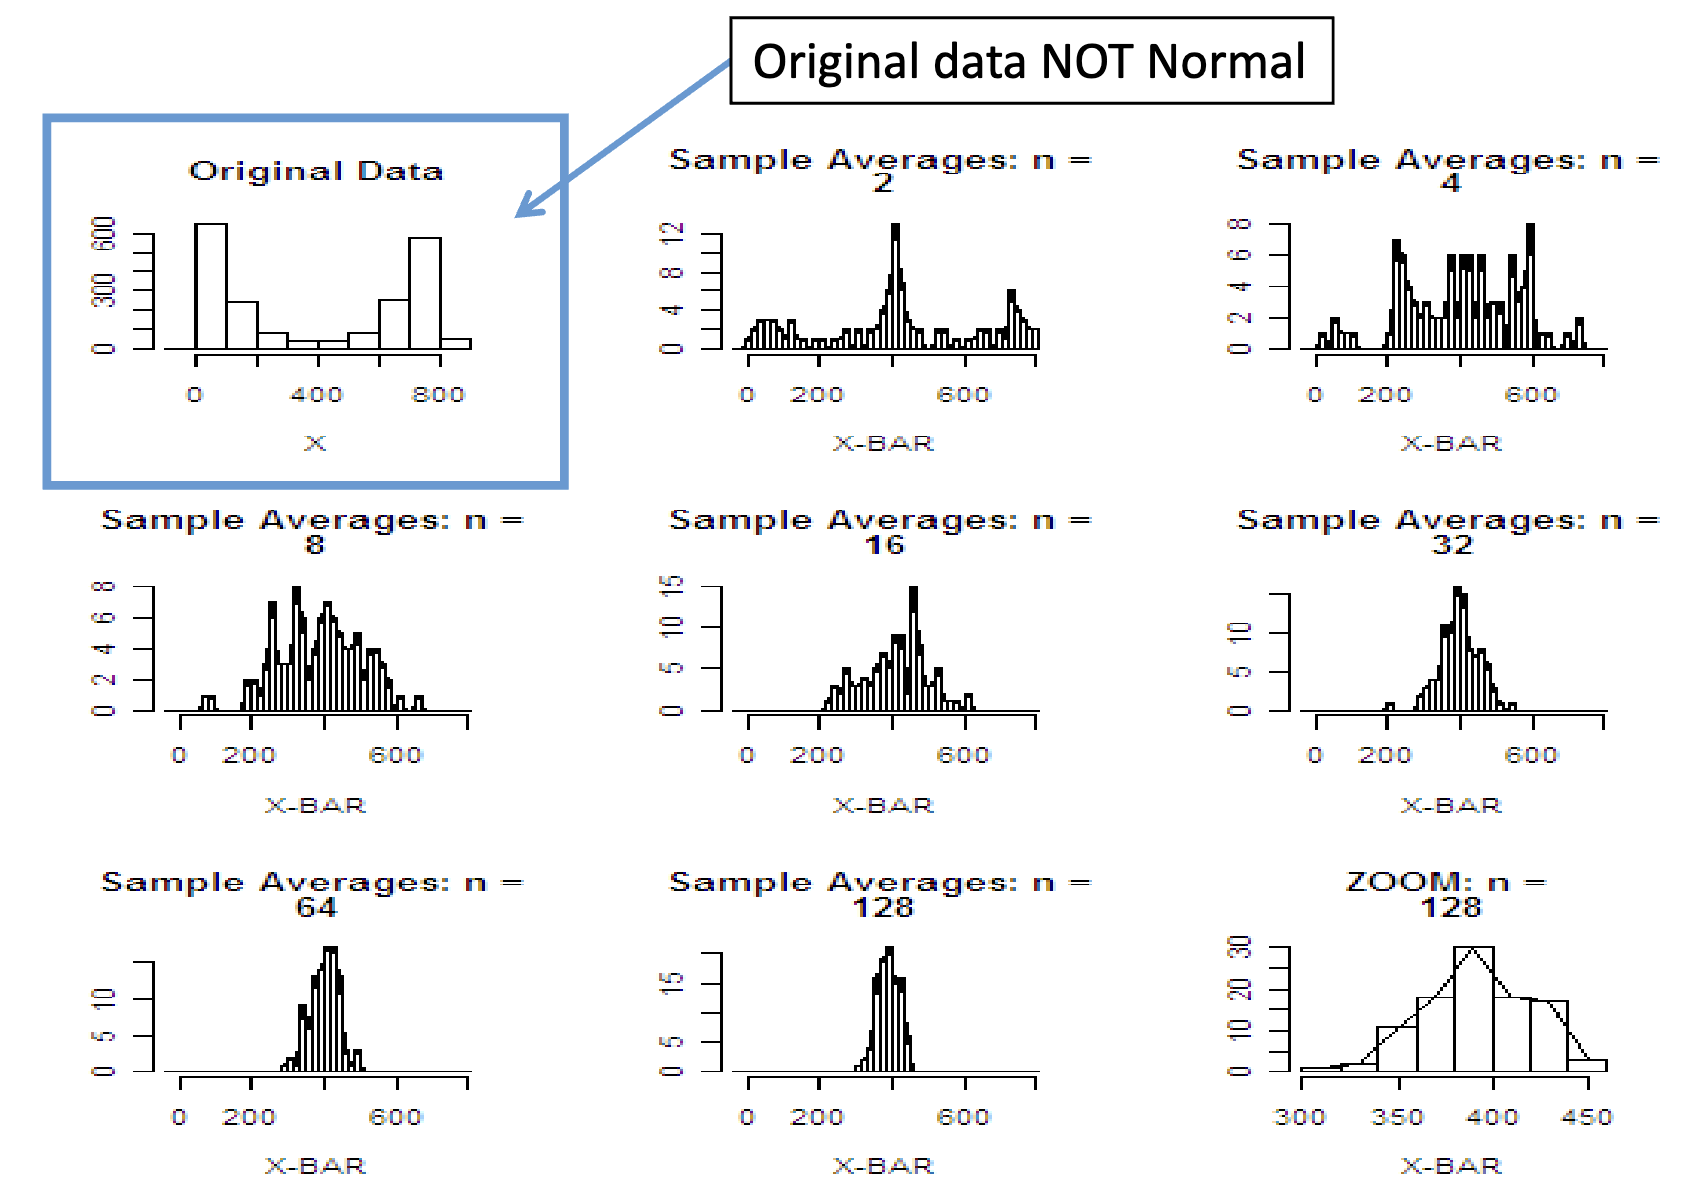
\includegraphics[scale=0.4]{img/CLT-ex.png}
    \caption{Visualizing the idea of CLT.}
\end{figure}

\begin{note}
    The distribution of sample means becomes normal as the sample size increases. Also, the sample mean converges to the population mean when $n$ becomes larger.
\end{note}


\pagebreak


\begin{example}
    Suppose fires reported to a fire station satisfy the conditions for a Poisson process, with a mean of 1 fire every 4 hours. Find the probability the $500^{\text{th}}$ fire of the year is reported on the $84^{\text{th}}$ day of the year.

    \textbf{Solution:} Let $X_i =$ time beteen $(i-1)^{\text{st}}$ and the $i^{\text{th}}$ fires ($X_1 =$ time to the first fire). Then, these $X_i$'s are independent and identically distributed as: $X_i \sim \text{Exp}(\theta = 4 \text{ hrs} = \frac{1}{6} \text{ day})$, since $\lambda = \frac{1}{4}$ fires per hour.

    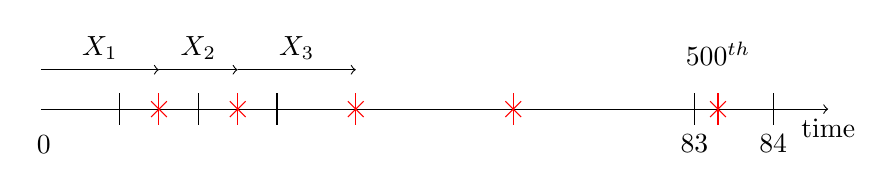
\begin{tikzpicture}
        % Draw the horizontal axis
        \draw[->] (0,0) -- (10,0) node[anchor=north] {time};
        
        % Draw the vertical lines and labels
        \foreach \x in {1, 2, 3} {
            \draw (\x,0.2) -- (\x,-0.2);
        }
        
        % Draw the crosses and labels for 83 and 84
        \foreach \x in {1.5, 2.5, 4, 6, 8.6} {
            \draw[red] (\x,0.2) -- (\x,-0.2);
            \draw[red] (\x-0.1,0.1) -- (\x+0.1,-0.1);
            \draw[red] (\x-0.1,-0.1) -- (\x+0.1,0.1);
        }
        
        \draw (8.3,0.2) -- (8.3,-0.2) node[anchor=north] {83};
        \draw (9.3,0.2) -- (9.3,-0.2) node[anchor=north] {84};
        
        % Draw the arrows for X1, X2, X3
        \draw[->] (0,0.5) -- (1.5,0.5) node[midway,above] {$X_1$};
        \draw[->] (1.5,0.5) -- (2.5,0.5) node[midway,above] {$X_2$};
        \draw[->] (2.5,0.5) -- (4,0.5) node[midway,above] {$X_3$};
        \node at (8.6,0.7) {$500^{\text{th}}$};
        
        % Add the 0 and 1 labels on the left
        \node[anchor=east] at (0.25,-0.45) {0};
        % \node[anchor=east] at (0.78,-0.45) {1};
    \end{tikzpicture}

    We want to find $P \left( 83 < \underbrace{\displaystyle \sum_{i=1}^{500} X_i}_{S_{500}} \leq 84 \right)$. By the Central Limit Theorem, $S_{500} = \displaystyle \sum_{i=1}^{500} X_i$ has approximately \vspace{-2mm}

    a $\text{N}(500\mu , 500\sigma^2) = \text{N}(\frac{500}{6}, \frac{500}{36})$ distribution. 
    \begin{align*}
        P(83 < S_{500} \leq 84) &\approx P \left( \frac{83 - \frac{500}{6}}{\sqrt{\frac{500}{36}}} < Z \leq \frac{84 - \frac{500}{6}}{\sqrt{\frac{500}{36}}} \right) \\
        &= P(-0.09 < Z \leq 0.19) \\
        &\vdots \\
        &= 0.57142 + 0.53586 - 1 \\
        &= 0.10728.
    \end{align*}
\end{example}

\begin{note}
    In this example, we used the normal distribution to approximate a continuous random variable (i.e. the exponential distribution). When approximating discrete random variables, we have to make a small adjustment, see next page!
\end{note}


\pagebreak


\begin{remark}[\textbf{Continuity Correction}]
    \phantom{}\\
    When approximating a discrete random variable, a slight adjustment is required to improve the approximation. 

For example, we are in a `100-cup challenge' where $P(\text{winning cup}) = \frac{1}{6}$, we bought 100 cups to see how many times we win. We want to find the probability of having between 15 to 20 winning cups. 

Let $X_i = $ whether the $i^{\text{th}}$ cup is a winning cup. Then $X_i \sim \text{Binomial}(n=1,p=\frac{1}{6})$ for $i = 1,2,\ldots,100$. And $\expect{X_i} = \frac{1}{6}$, $\Var{X_i} = \frac{5}{36}$, with $S_{100} = \displaystyle \sum_{i=1}^{100} X_i = $ total number of winning cups. By the CLT, we have $S_{100}$ approximately have $\text{N}(\frac{100}{6}, \frac{500}{36})$, we'll see a theorem below about this. Then,
\[
    P(15 \leq S_{100} \leq 20) = P(-0.447 \leq Z \leq 0.894) = 0.487.
\]
If we compute the exact probability using $S_{100} \sim \text{Binomial}(100, \frac{1}{6})$, we get $P(15 \leq S_{100} \leq 20) = 0.561$. This is quite off!

Since $X_i$ are discrete, so $S_{100}$ is also discrete and cannot take non-integer values. In this case, the approximation is underestimate as seen in Figure 14 (part of $X=15$ and $X = 20$ are not included by the normal approximation in {\color{blue} blue}), so subtract 0.5 to get $P(14.5 \leq S_{100} \leq 20.5)$, which gives a better approximation.

\begin{figure}[!htb]
    \begin{minipage}{0.5\textwidth}
      \centering
      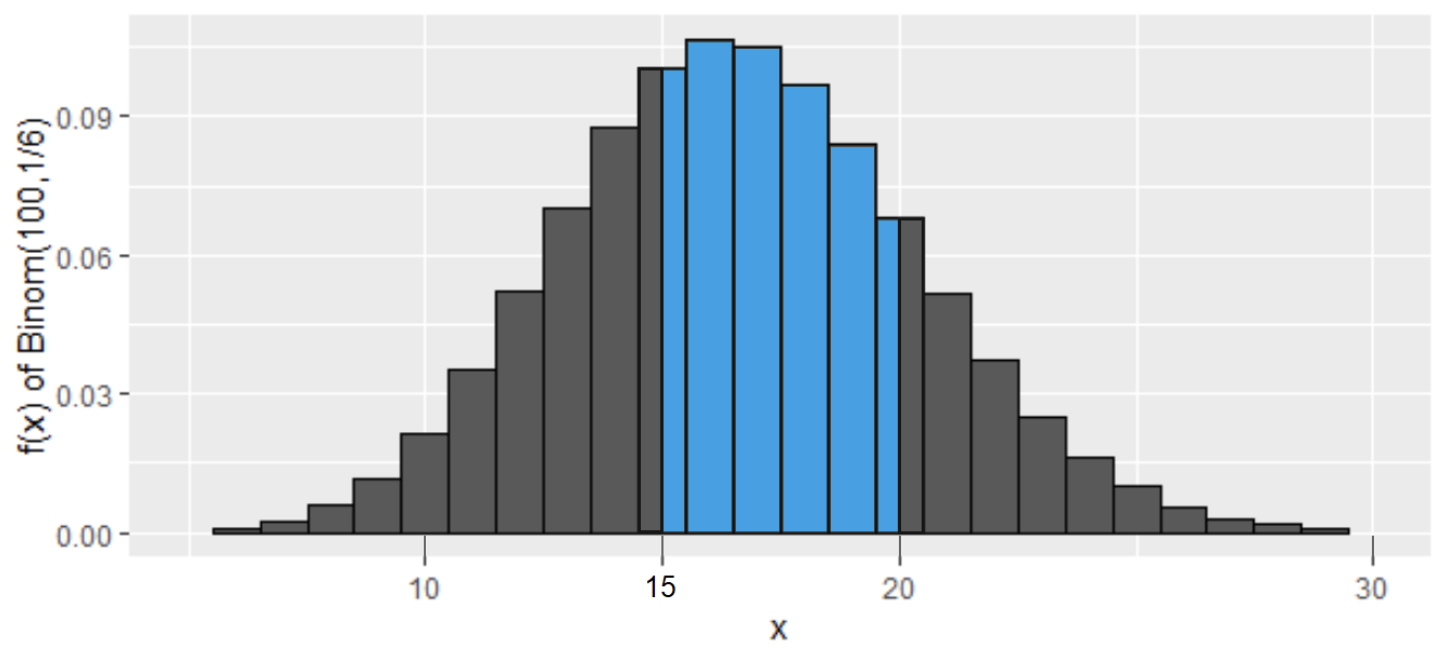
\includegraphics[width=1\linewidth]{img/without-adjustment.png}
      \caption{Without adjustment (underestimate).}
    \end{minipage}\hfill
    \begin{minipage}{0.5\textwidth}
      \centering
      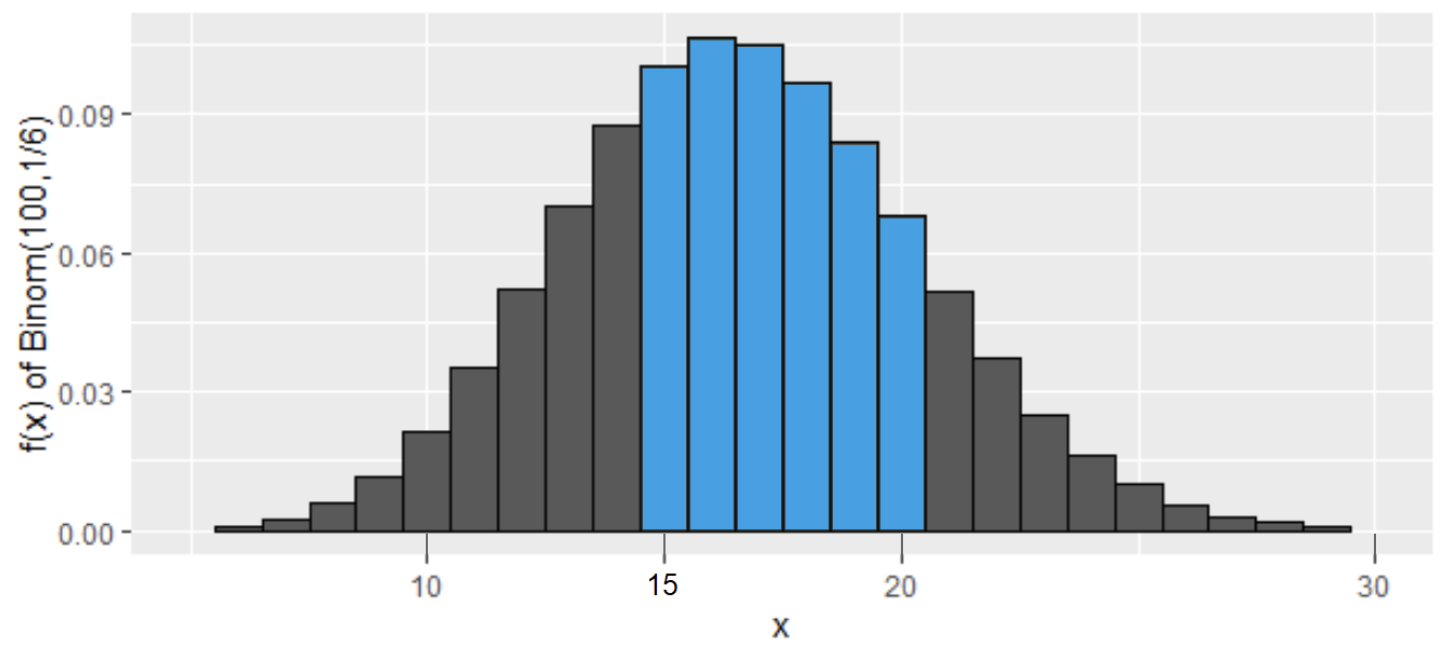
\includegraphics[width=1\linewidth]{img/with-adjustment.png}
      \caption{With adjustment (better).}
    \end{minipage}
 \end{figure}

 $P(14.5 \leq S_{100} \leq 20.5) = 0.568$, which is way better!

 This adjustment is called the ``\textbf{Continuity Correction}''.
\end{remark}

\begin{note}
    \phantom{}
    \begin{itemize}
        \item It is only applied when using a \textbf{continous} distribution to approximate a \textbf{discrete} one.
        \item Quick sketch to see whether to add or subtracct 0.5 (see below proposition).
    \end{itemize}
\end{note}

\begin{proposition}[\textbf{Continuity Correction Rules}]
    \phantom{}\
    \begin{itemize}
        \item $P(X > n)$, use $P(X > n + 0.5)$.
        \item $P(X \geq n)$, use $P(X > n - 0.5)$.
        \item $P(X > n)$, use $P(X < n - 0.5)$.
        \item $P(X \leq n)$, use $P(X < n + 0.5)$.
        \item $P(a < X < b)$, use $P(a + 0.5 \leq X \leq b - 0.5)$.
        \item $P(a \leq X \leq b)$, use $P(a - 0.5 \leq X \leq b + 0.5)$.
        \item $P(X = n)$, use $P(n-0.5 \leq X \leq n + 0.5)$.
    \end{itemize}
\end{proposition}

\begin{theorem}[\textbf{Normal Approximation to Poisson}]
    \phantom{}  \\
    Suppose $X \sim Poisson(\mu)$. Then the cumulative distribution function of the standarized
    random variable \vspace{-2mm}
    \[Z = \frac{X - \mu}{\sqrt{\mu}}\]
    approaches that of a standard Normal random variable as $\mu \to \infty$.
\end{theorem}

\begin{remark}
    We have $X \sim \text{N}(\mu,\mu)$, where $\mu = \lambda t$. Approximation will be good when $\mu > 5$.
\end{remark}

\begin{theorem}[\textbf{Normal Approximation to Binomial}]
    \phantom{}  \\
    Suppose $X \sim Binomial(n, p)$. Then for large $n$, the random variable \vspace{-1mm}
    \[W = \frac{X - np}{\sqrt{np(1 - p)}}\]
    has approximately a $N(0, 1)$ distribution.
\end{theorem}

\begin{remark}
    We write $\frac{X - np}{\sqrt{np(1 - p)}} \sim \text{N}(0,1)$ or $X \sim \text{N}(np,np(1-p))$. \vspace{-1mm} \\
\end{remark}


\begin{example}
    Suppose $X \sim \text{Poisson}(9)$. Use the Normal approximation to approximate $P(X > 9)$, and cpmare with the true value.

    By Normal approximation to Poisson, we have $Z = \frac{X-\mu}{\sqrt{\mu}}$. Using continuity correction, \vspace{-3mm}
    \[
        P(X > 9) \approx P(X > 9 \text{ } {\color{blue} + \text{ } 0.5}) = P \left( Z > \frac{9.5 - 9}{\sqrt{9}} \right) = P(Z > 0.17) = 0.4324.
    \]
    Note: the true value is 0.4126.
\end{example}

\begin{example}
    Suppose $X \sim \text{Binomial}(20,0.4)$. Find the approximate probability $P(4 \leq X \leq 12)$ and compare it to the true value.

    \textbf{Solution:} Note that $\expect{X} = np = 8$ and $\Var{X} = np(1-p) = 4.8$. By the Normal approximation to the Binomial, we have $X \sim \text{N}(8,4.8)$ approximately.
    \begin{align*}
        P(4 \leq X \leq 12) &\approx P(4 \text{ } {\color{blue} - \text{ } 0.5} \leq X \leq 12 \text{ } {\color{blue} + \text{ } 0.5}) \\
        &= P \left( \frac{3.5 - 8}{\sqrt{4.8}} \leq \frac{X - 8}{\sqrt{4.8}} \leq \frac{12.5 - 8}{\sqrt{4.8}} \right) \\
        &= P(-2.054 \leq Z \leq 2.054) \\
        &\vdots \\
        &= 0.96.
    \end{align*}
    Note: the true value is $\displaystyle \sum_{x=4}^{12} \binom{20}{x} (0.4)^x (0.6)^{20-x} = 0.963$. \\
\end{example}

\begin{example}
    Let $p$ be the proportion of Canadians who think Canada should adopt the US dollar.
    \begin{enumerate}[label=(\alph*)]
        \item Suppose 400 Canadians are randomly chosen and asked their opinion. Let $X$ be the number who say yes. Find the probability that the proportion, $X/400$, of people who say yes is within 0.02 of $p$, if $p$ is 0.20.
        \quad \textbf{Ans:} $2P(Z < 1.06) - 1 = 0.711$.
        \item Find the number, n, who must be surveyed so there is a $95\%$ chance that $X/n$ lies within 0.02 of $p$, when $p$ is unknown.
        
        \textbf{Ans:} $Z = 1.96 = \frac{0.02}{\sqrt{\frac{p(1-p)}{n}}}$. Set $(p(1-p))^\prime = 0$ to find the max $p = 0.5$. Sub in $p = 0.5$ to get $n = 2401$, and this works for all $p$ since it works for the max $p$.
    \end{enumerate}
\end{example}

\pagebreak

\subsection{Moment Generating Functions}

So far, we have seen two functions which characterize a distribution of a random variable:
\begin{itemize}
    \item p.d.f.
    \item c.d.f.
\end{itemize}
However, there is a third function which also \textbf{uniquely} determines a distribution: the \textbf{moment generating function}.


\begin{definition}[\textbf{Moment Generating Functions for Discrete}]
    \phantom{}\\
    Consider a discrete random variable $X$ with probability function $f(x)$. The moment generating function (m.g.f.) of $X$ is defined as \vspace{-3mm}
    \[
        M(t) = \expect{e^{tX}} = \displaystyle \sum_{\text{all $x$}} e^{tx} f(x).
    \]
    We will assume that the moment generating function is defined and finite for values of $t$ in an interval around 0 (i.e. for some $a > 0$, $\displaystyle \sum_{x} e^{tx} f(x) < \infty \; \forall t \in [-a,a]$).
\end{definition}

The m.g.f. of $X$ can be used to evaluate the moments of the random variable $X$, where the \textbf{moments} of $X$ are defined as the \textbf{expectations} of the functions $X^k$ for $k = 1,2,\ldots$. \vspace{-3mm}
\[
    \expect{X^k} \text{ is the $k^{\text{th}}$ moment of $X$.}
\]

\vspace{-3mm}

\begin{example}
    \phantom{}\
    \begin{itemize}
        \item The mean $\mu = \expect{X}$ is the first moment of $X$.
        \item $\expect{X^2}$ is the second moment of $X$ and so on.
    \end{itemize}
\end{example}

\vspace{2mm}

\begin{theorem}
    \phantom{}\\
    Suppose the random variable $X$ has moment generating function $M(t)$ defined $\forall t \in [-a,a]$ for some $a > 0$. Then \vspace{-3mm}
    \[
        \expect{X^k} = M^{(k)}(0) \quad \text{for $k = 1,2,\ldots$}
    \]
    where $M^{(k)}(0) = \dis \frac{\dd^k}{\dd{t^k}} M(t) \, |_{t=0} \quad \text{for } k = 1, 2, \ldots$
\end{theorem}

\pagebreak

\begin{example}[\textbf{MGF for Binomial}]
    \phantom{}\\
    Suppose $X \sim \text{Binomial}(n,p)$. Then its moment generating function is
    \begin{align*}
        M(t) &= \displaystyle \sum_{x=0}^{n} e^{tx} \binom{n}{x} p^x (1-p)^{n-x} \\
        &= \displaystyle \sum_{x=0}^{n} \binom{n}{x} (p e^t)^x (1-p)^{n-x} \\
        &=(pe^t + 1 - p)^n \quad \text{by the Binomial Theorem $\forall t$.}
    \end{align*}
    Therefore, \vspace{-3mm}
    \begin{align*}
        M^\prime(t) &= npe^t \left(pe^t + 1 - p\right)^{n-1} \\
        M^\dprime(t) &= npe^t \left(pe^t + 1 - p\right)^{n-1} + n(n-1)p^2 e^{2t} \left(pe^t + 1 - p\right)^{n-2}
    \end{align*}
    and so
    \begin{align*}
        \expect{X} &= m^\prime(0) = np \\
        \expect{X^2} &= M^\dprime(0) = np + n(n-1)p^2 \\
        \Var{X} &= \expect{X^2} - \left( \expect{X} \right)^2 = np(1-p).
    \end{align*}
\end{example}

\begin{example}[exercise]
    Find the m.g.f. for a Poisson distrubition $X \sim \text{Poisson}(\mu)$. \\
\end{example}

\begin{theorem}[\textbf{Uniqueness Theorem for MGFs}]
    \phantom{}\\
    Suppose that random variables $X$ and $Y$ have moment generating functions $M_X(t)$ and $M_Y(t)$, respectively. If $M_X(t) = M_Y(t) \; \forall t$, then $X$ and $Y$ have the same distribution.
\end{theorem}

The m.g.f. uniquely identifies a distribution. For example, if $X$ has m.g.f.: $e^{2(e^t -1)}$. Then, you can immediately tell that $X \sim \text{Poisson}(2)$.

MGFs can also be used to determine that a sequence of distributions gets closer and closer to some limiting distribution. To show this, suppose that a sequence of probability functions $f_n(x)$ have corresponding moment generating functions: \vspace{-3mm}
\[
    M_n(t) = \displaystyle \sum_{\text{all $x$}} e^{tx} f_n(x).
\]
And suppose that the probability functions $f_n(x)$ converge to another probability function $f(x)$ pointwise in $x$ as $n \to \infty$. Then since
\vspace{-3mm}
\[
    f_n(x) \to f(x) \text{ as $n \to \infty$ for each $x$},
\]
we have \vspace{-3mm}
\[
    \sum_{\text{all $x$}} e^{tx} f_n(x) \to \sum_{\text{all $x$}} e^{tx} f(x) \text{ as $n \to \infty$ for each $t$}.
\]
In other words, $M_n(t)$ converges to $M(t)$, the moment generating function of the limiting distribution.

\textbf{Note:} The converse also holds. Suppose that $X_n$ has m.g.f. $M_n(t)$ and $M_n(t) \to M(t)$ for each $t$, such that $M(t) < \infty$, then
\vspace{-3mm}
\[
    f_n(x) \to f(x) \text{ as $n \to \infty$ for each $x$}.
\]

\begin{example}
    The Poisson approximation of the Binomial distribution when $n$ is very large and $p$ is close to 0.

    $\mu = np \implies p = \frac{\mu}{n}$. Then, the m.g.f. of such a Binomial random variable:
    \begin{align*}
        M(t) &= (pe^t + 1 - 1)^n \\
        &= \left[ 1 + p(e^t -1) \right]^n \\
        &= \left[ 1 + \frac{\mu}{n} (e^t -1) \right]^n.
    \end{align*}
    Now, take the limit of this expression as $n \to \infty$. Since $\dis \lim_{n \to \infty} \left( 1 + \frac{c}{n} \right)^n \to e^c$, we have
    \[
        \lim_{n \to \infty} \left[ 1 + \frac{\mu}{n} (e^t -1) \right]^n = e^{\mu(e^t -1)},
    \]
    and this is the m.g.f. of a Poisson distribution with parameter $\mu$. This shows a little more formally that the Binomial distribution with small $p$ and large $n$ approaches the Poisson distribution with $\mu = np$  as $n \to \infty$.
\end{example}

\pagebreak

\textbf{Moment Generating Function of a Continuous Random Variable}

\begin{definition}[\textbf{Moment Generating Functions for Continous}]
    \phantom{}\\
    Consider a continuous random variable $X$ with probability density function $f(x)$. Then moment generating function of $X$ is defined as
    \vspace{-3mm}
    \[
        M(t) = \expect{e^{tx}} = \displaystyle \int_{-\infty}^{\infty} e^{tx} f(x) \, dx.
    \]
    We will assume that the m.g.f. is defined and finite for values of $t$ in an interval around 0. That is, for some $a > 0$, $\displaystyle \int_{-\infty}^{\infty} e^{tx} f(x) \, dx < \infty \; \forall t \in [-a,a]$.
\end{definition}

\begin{example}
    Suppose that $X \sim \text{Exponential}(\theta)$. Show that the m.g.f. is given by \vspace{-3mm}
    \[
        M(t) = \frac{1}{1 - \theta t} \quad \text{for $t < \frac{1}{\theta}$}.
    \]
    \textbf{Solution:} Recall that $\Gamma(\alpha) = \displaystyle \int_{0}^{\infty} x^{\alpha -1} e^{-x} \, dx$. By definition, we have \vspace{-3mm}
    \begin{align*}
        M(t) &= \displaystyle \int_{0}^{\infty} e^{tx} \lambda e^{-\lambda x} \, dx \\
        &= \lambda \displaystyle \int_{0}^{\infty} x^{1-1} e^{-x(\lambda - t)} \, dx \quad \text{let $u = x(\lambda - t)$}, dx = \frac{du}{\lambda - t} \\
        &= \dis \frac{\lambda}{\lambda - t} \displaystyle \int_{0}^{\infty} \left( \frac{u}{\lambda - t} \right)^{1-1} e^{-u} \, dx \\
        &= \dis \frac{\lambda}{\lambda - t} \displaystyle \int_{0}^{\infty} u^{1-1} e^{-u} \, dx \\
        &= \dis \frac{\lambda}{\lambda - t} \cdot \Gamma(1) \\
        &= \dis \frac{\lambda}{\lambda - t} \\
        &= \dis \frac{1}{1 - \theta t} \quad \text{since $\theta = \frac{1}{\lambda}$}.
    \end{align*}
    Notice that $\lambda - t > 0$ is necessary for the integral to converge, so we have $t < \lambda = \frac{1}{\theta}$.
\end{example}

\pagebreak

\begin{proposition}[\textbf{Summary of MGFs}]
    \phantom{}\\
    For discrete random variables:
    \begin{itemize} \itemsep 1.5pt
        \item If $X \sim \text{Binomial}(n,p)$, then $M(t) = (pe^t + 1 - p)^n$, $t \in \R$.
        \item If $X \sim \text{Poisson}(\mu)$, then $M(t) = e^{\mu (e^t -1)}$, $t \in \R$.
        \item If $X \sim \text{NB}(k,p)$, then $\dis M(t) = \left( \frac{p}{1- (1-p)e^t} \right)^k$, $t < - \ln(1-p)$.
        \item If $X \sim \text{Geometric}(p)$, then $\dis M(t) = \frac{p}{1- (1-p)e^t}$, $t < - \ln(1-p)$.
    \end{itemize}
    For continuous random variables:
    \begin{itemize} \itemsep 1.5pt
        \item If $X \sim \text{U}(k,p)$, then $\dis M(t) = \frac{e^{bt} - e^{at}}{(b-a)t}$, $t \neq 0$.
        \item If $X \sim \text{Exponential}(\theta)$, then $\dis M(t) = \frac{1}{1- \theta t}$, $t < - \frac{1}{\theta}$.
        \item If $X \sim \text{NB}(k,p)$, then $\dis M(t) = e^{\mu t + \frac{\sigma^2 t^2}{2}}$, $t \in \R$.
    \end{itemize}
\end{proposition}

\phantom{}\\

\subsection{Motivariate Moment Generating Functions}

Did-not-have-time-to-cover material. \\
\phantom{}\\
\phantom{}\\
\phantom{}\\
\phantom{}\\
\phantom{}\\
\phantom{}\\
\phantom{}\\
\phantom{}\\
\phantom{}\\
\phantom{}\\
\phantom{}\\
\phantom{}\\
\phantom{}\\
% \vspace{0.5mm}

\begin{center}
    {\LARGE END OF STAT 230!}
\end{center}



\newpage



\end{document}